\documentclass[12pt,a4paper]{report}

\usepackage[T1]{fontenc}
\usepackage[utf8]{inputenc}
\usepackage[italian]{babel}
\usepackage{bold-extra}
\usepackage{tocloft}
\usepackage{multicol} % http://ctan.org/pkg/multicols
\usepackage{titlesec}
\usepackage{float}
\usepackage{amsmath}
\usepackage{hyperref}
\usepackage{graphicx}
\usepackage{listings}
\usepackage{minted}
\usepackage{verbatim}
\usepackage[dvipsnames]{xcolor}
\usepackage[toc,page]{appendix}
\usepackage{fancyhdr}

\usepackage[
  top=3cm,
  bottom=3cm,
  left=2cm,
  right=3cm,
  headheight=17pt, % as per the warning by fancyhdr
  includehead,includefoot,
  heightrounded
]{geometry}

% !TeX root = main.tex

\textwidth=450pt
\oddsidemargin=0pt

\setcounter{tocdepth}{3}
\setcounter{secnumdepth}{3}

\renewcommand{\cftpartleader}{\cftdotfill{\cftdotsep}} % for parts
\renewcommand{\cftchapleader}{\cftdotfill{\cftdotsep}} % for chapters

\titleformat{\chapter}{\Huge\bfseries}{\chaptername\ \thechapter}{0pt}{\vskip 100pt\raggedright}%
% Alter <after-sep> in the macro below to vary the separation after the \chapter title.
\titlespacing{\chapter}{0pt}{50pt}{50pt}
% \titlespacing{<command>}{<left>}{<before-sep>}{<after-sep>}[<right>]

% configura i lettori pdf
\hypersetup{%
  pdfpagemode={UseNone},
  hidelinks,                  % nasconde i collegamenti (non vengono quadrettati)
  hypertexnames=false,
  linktoc=all,                % inserisce i link nell'indice
  unicode=true,               % usa solo caratteri Latini nei segnalibri di Acrobat
  pdftoolbar=false,           % nasconde la toolbar di Acrobat
  pdfmenubar=false,           % nasconde il menu di Acrobat
  plainpages=false,
  breaklinks,
  pdfstartview={Fit},
  pdflang={it}
}

\lstdefinelanguage{Kotlin}{
  comment=[l]{//},
  commentstyle={\color{gray}\ttfamily},
  emph={filter, first, firstOrNull, forEach, lazy, map, mapNotNull, println},
  emphstyle={\color{OrangeRed}},
  identifierstyle=\color{black},
  keywords={!in, !is, abstract, actual, annotation, as, as?, break, by, catch, class, companion, const, constructor, continue, crossinline, data, delegate, do, dynamic, else, enum, expect, external, false, field, file, final, finally, for, fun, get, if, import, in, infix, init, inline, inner, interface, internal, is, lateinit, noinline, null, object, open, operator, out, override, package, param, private, property, protected, public, receiveris, reified, return, return@, sealed, set, setparam, super, suspend, tailrec, this, throw, true, try, typealias, typeof, val, var, vararg, when, where, while},
  keywordstyle={\color{NavyBlue}\bfseries},
  morecomment=[s]{/*}{*/},
  morestring=[b]",
  morestring=[s]{"""*}{*"""},
  ndkeywords={@Deprecated, @JvmField, @JvmName, @JvmOverloads, @JvmStatic, @JvmSynthetic, Array, Byte, Double, Float, Int, Integer, Iterable, Long, Runnable, Short, String, Any, Unit, Nothing},
  ndkeywordstyle={\color{BurntOrange}\bfseries},
  sensitive=true,
  stringstyle={\color{ForestGreen}\ttfamily},
}

\setminted[terraform]{
  linenos=true,
  breaklines=true,
  encoding=utf8,
  fontsize=\footnotesize,
  frame=lines
}

\setminted[java]{
  linenos=true,
  breaklines=true,
  encoding=utf8,
  fontsize=\footnotesize,
  frame=lines
}

\setminted[docker]{
  linenos=true,
  breaklines=true,
  encoding=utf8,
  fontsize=\footnotesize,
  frame=lines
}

\setminted[yaml]{
  linenos=true,
  breaklines=true,
  autogobble,
  encoding=utf8,
  fontsize=\footnotesize,
  frame=lines
}

\setminted[bash]{
  linenos=true,
  breaklines=true,
  autogobble,
  encoding=utf8,
  fontsize=\footnotesize,
  frame=lines
}

\setminted[toml]{
  linenos=true,
  breaklines=true,
  autogobble,
  encoding=utf8,
  fontsize=\footnotesize,
  frame=lines
}

\setminted[kotlin]{
  linenos=true,
  breaklines=true,
  autogobble,
  encoding=utf8,
  fontsize=\footnotesize,
  frame=lines
}

\setminted[ruby]{
  linenos=true,
  breaklines=true,
  encoding=utf8,
  fontsize=\footnotesize,
  frame=lines
}

\begin{document}
  
\begin{titlepage}
\begin{center}
{{\Large{\textsc{Alma Mater Studiorum $\cdot$ Universit\`a di
Bologna\\\vspace{2mm}Campus di Cesena}}}} 
\rule[0.1cm]{15.8cm}{0.1mm}
\rule[0.5cm]{15.8cm}{0.6mm}

{\small{\textsc { DIPARTIMENTO DI INFORMATICA – SCIENZA E INGEGNERIA \\
\vspace{3mm}
Corso di Laurea Magistrale in Ingegneria e scienze informatiche}}}
\end{center}
\vspace{15mm}
\begin{center}
{\LARGE\textbf{DEVOPS PER APPLICAZIONI MOBILE}} \\
\vspace{3mm}
{\LARGE\textbf{MULTIPIATTAFORMA: UN CASO DI}} \\
\vspace{3mm}
{\LARGE\textbf{STUDIO INDUSTRIALE}} \\
\vspace{20mm} {\large{\sc Tesi di Laurea Magistrale in\\ Laboratorio di Sistemi Software LM}}
\end{center}
\vfill
\par
\noindent

\begin{minipage}[t]{0.47\textwidth}
{\large{\sc Relatore:}\\
{\bf \textsc{Prof. Danilo Pianini}}}\\ \\
{\large{\sc Correlatore:}\\
{\bf \textsc{Prof.ssa Catia Prandi}}}\\
\vskip 8pt
\end{minipage}
\hfill
\begin{minipage}[t]{0.47\textwidth}\raggedleft
{\large{\sc Presentata da:}\\
%\vspace{2mm}
{\bf Filippo Paganelli}}
\end{minipage}
\vspace{20mm}
\begin{center}
\rule[0.1cm]{15.8cm}{0.2mm}
{\large{\sc III Sessione\\
Anno Accademico 2021/2022}}
\end{center}
\end{titlepage}

\newpage

\begin{center}
{\LARGE{\bf Sommario}}
\end{center}
{
\noindent
% !TeX root = ../main.tex

\parindent=0pt
Nonostante la presenza di diversi team dedicati allo sviluppo di applicazioni mobile all'interno del Gruppo Maggioli, non esiste un chiaro processo standard a livello aziendale per lo sviluppo di applicazioni mobile. La situazione è invece differente per la maggior parte degli altri team che si occupano dello sviluppo di altre tipologie di applicazioni, come ad esempio Web Application, per i quali invece esiste un processo ben definito e collaudato a livello aziendale.\\
Questo progetto di tesi magistrale consiste ($i$) nella progettazione di un primo modello di standard aziendale per il processo di sviluppo delle applicazioni mobile tale da poter essere adottato dagli altri team in Maggioli, ($ii$) nella applicazione delle pratiche di automazione DevOps a tale processo e ($iii$) nella dimostrazione della sua efficacia tramite lo sviluppo di una applicazione PoC con lo scopo di aumentare la conoscenza e l'esperienza in ambito applicazioni mobile del team di Ricerca e Sviluppo.\\
Il primo task svolto, descritto nel capitolo \ref{ch:ch2}, ha l'obiettivo di definire i vari passi che compongono il tipico processo di sviluppo di applicazioni mobile basandosi sia sulle tecniche attualmente adottate dai team in Maggioli che dalle best practice individuate in letteratura. Successivamente sono stati scelti gli strumenti necessari per soddisfare i requisiti dettati dal processo di sviluppo. Nel capitolo \ref{ch:ch3} sono descritti gli strumenti core utilizzati nel processo di sviluppo (\textit{GitLab} e \textit{Fastlane}) e nello sviluppo della applicazione PoC (\textit{Kotlin Multiplatform Mobile}). Definito il processo e i tool, viene descritto nel capitolo \ref{ch:ch4} come sono state adpttate le pratiche DevOps e in particolare \textit{Continuous Integration}, \textit{Continuous Delivery} e \textit{Continuous Inspection}. L'obiettivo è quello di integrare in modo più frequente piccole modifiche (integration) riducendo il tempo che intercorre tra la modifica del codice e l'effettivo rilascio (delivery) della applicazione sullo store della relativa piattaforma target, con un aumento della qualità e della sicurezza (inspection). Realizzato il sistema a supporto del processo di sviluppo, quest'ultimo è stato testato tramite lo sviluppo di una applicazione PoC, chiamata \textit{MaggioliEbook}, descritta nel capitolo \ref{ch:ch5}. L'applicazione rappresenta un primo passo per l'azienda verso una nuova modalità di fruizione e consultazione dei propri contenuti editoriali digitali in formato EPUB e su dispostivi mobile. Infine nel capitolo \ref{ch:ch6} sono analizzati i risultati ottenuti da questo progetto di tesi e indicati possibili lavori futuri che verranno svolti.

\addcontentsline{toc}{chapter}{Sommario}
}

\newpage

\tableofcontents

\setlength{\parindent}{0em}

\chapter{Applicazioni Multipiattaforma}
\label{ch:ch1}
% !TeX root = ../main.tex

\section{Introduzione}
La continua crescita della quantità di dispositivi mobile presenti, e in particolare gli smartphone, ha reso molto importante a livello globale il mercato delle applicazioni e per questo motivo sono sempre di più le aziende che decidono di investire risorse nello sviluppo e nella vendita di applicazioni mobile. Una azienda che intende targettizzare il maggior numero di utenti possibile con le proprie applicazioni deve considerare che l'intero mercato è spartito in base alla diffusione dei sistemi operativi per smartphone. Ad oggi, i sistemi operativi più diffusi sono Android (Google) e iOS (Apple), i quali coprono quasi la totalità del mercato con quote rispettivamente del 71\% e del 28\%\footnote{\href{https://www.statista.com/statistics/272698/global-market-share-held-by-mobile-operating-systems-since-2009/}{https://www.statista.com/statistics/272698/global-market-share-held-by-mobile-operating-systems-since-2009/}}. Questi dati comportano per una azienda la necessità di sviluppare la stessa applicazione per almeno due piattaforme completamente differenti tra loro. A tal proposito sono nate nuove metodologie e tecniche basate sul concetto "Write Once, Run Anywhere" (WORA)\footnote{\href{https://www.computerweekly.com/feature/Write-once-run-anywhere}{https://www.computerweekly.com/feature/Write-once-run-anywhere}} con lo scopo di ottimizzare lo sviluppo delle applicazioni mobile al fine di ridurre i costi e aumentare l'efficienza del processo di sviluppo.

Le principali tecniche moderne di sviluppo per applicazioni mobile sono:
\begin{itemize}
    \item \textbf{Cross-platform} - Rispetta completamente la filosofia WORA. Lo stesso codice può essere eseguito su diverse piattaforme grazie ad uno strato applicativo aggiuntivo che si occupa di interpretare il codice e tradurlo nel linguaggio specifico della piattaforma target.
    \item \textbf{Multi-platform} - Tecnica più recente che permette di sviluppare applicazioni native condividendo solamente la logica applicativa. In questo caso non è necessario uno strato software aggiuntivo perchè la applicazione può essere eseguita direttamente dalla piattaforma target.
\end{itemize}

\section{Cross-platform vs Multi-platform}
Sia nel caso cross-platform che nel caso multi-platform i principali vantaggi, che sono la riduzione dei costi e l'ottimizzazione del processo di sviluppo, derivano dalla condivisione e dal riuso del codice e quindi meno risorse impiegate rispetto allo sviluppo classico delle applicazioni mobile native.

Esistono però alcune differenze tra loro, fondamentali durante la scelta della metodologia da adottare da parte di una azienda per lo sviluppo di una applicazione mobile.
\begin{itemize}
    \item \textbf{Cross-platform}
    \begin{itemize}
        \item Condivisione/riuso totale del codice. Sia la logica applicativa che l'interfaccia utente sono le stesse per qualsiasi piattaforma.
        \item Performance limitate rispetto al nativo, dovute dalla presenza di uno strato software aggiuntivo che interpreta e traduce il codice.
        \item Accesso alle funzionalità hardware del dispositivo limitato e/o con overhead, dovuto sempre dalla presenza dello strato software aggiuntivo.
    \end{itemize}
    \item \textbf{Multi-platform}
    \begin{itemize}
        \item Condivisione/riuso della sola logica applicativa. Lo sviluppo dell'interfaccia utente rimane nativo.
        \item Performance elevate, equivalenti a quelle native.
        \item Accesso completo e senza overhead a tutte le funzionalità hardware del dispositivo.
    \end{itemize}
\end{itemize}

\section{Strumenti}
\label{app-multiplatform-tools}
Tipicamente quando ci si approccia allo sviluppo di una qualsiasi tipologia di software si effettua una ricerca di tutti gli strumenti in grado di facilitare il lavoro dello sviluppatore. Le principali categorie di strumenti necessari sono: (\textit{i}) linguaggio di programmazione, (\textit{ii}) ambiente di sviluppo (IDE\footnote{Integrated Development Environment}), (\textit{iii}) build automation e (\textit{iv}) framework di sviluppo.

La scelta di questi strumenti è spesso vincolata dalla piattaforma target, ovvero l'ambiente dove eseguirà il codice, e lo è in particolare per le applicazioni mobile. A differenza dello sviluppo di applicazioni Android, dove gran parte degli strumenti più diffusi è open-source, lo sviluppo di applicazioni iOS richiede vincoli stringenti imposti da Apple come ad esempio l'utilizzo dell'IDE XCode, il quale è disponibile solamente per il sistema operativo macOS.

Per gli strumenti di build automation esistono diverse alternative per l'ecosistema Android, anche se lo standard de-facto è dato dal tool Gradle. Lo stesso non è vero invece per le applicazioni iOS: come per l'IDE anche in questo caso è necessario utilizzare un insieme di tool specifici indicati da Apple. I più popolari frameworks open-source per lo sviluppo di applicazioni cross-platform sono: (\textit{i}) Ionic, (\textit{ii}) Flutter e (\textit{iii}) React Native. Il paradigma multi-platform è più recente rispetto al quello cross-platform e il principale framework open-source in questo caso è Kotlin Multiplatform.

\subsection{Kotlin Multiplatform Mobile}
Kotlin Multiplatform Mobile\footnote{\href{https://kotlinlang.org/lp/mobile/}{https://kotlinlang.org/lp/mobile/}} (KMM) è un framework per lo sviluppo di applicazioni Android e iOS basato sul concetto di condivisione della logica applicativa mantenendo lo sviluppo nativo della UX/UI.

\begin{figure}[H]
    \centering
    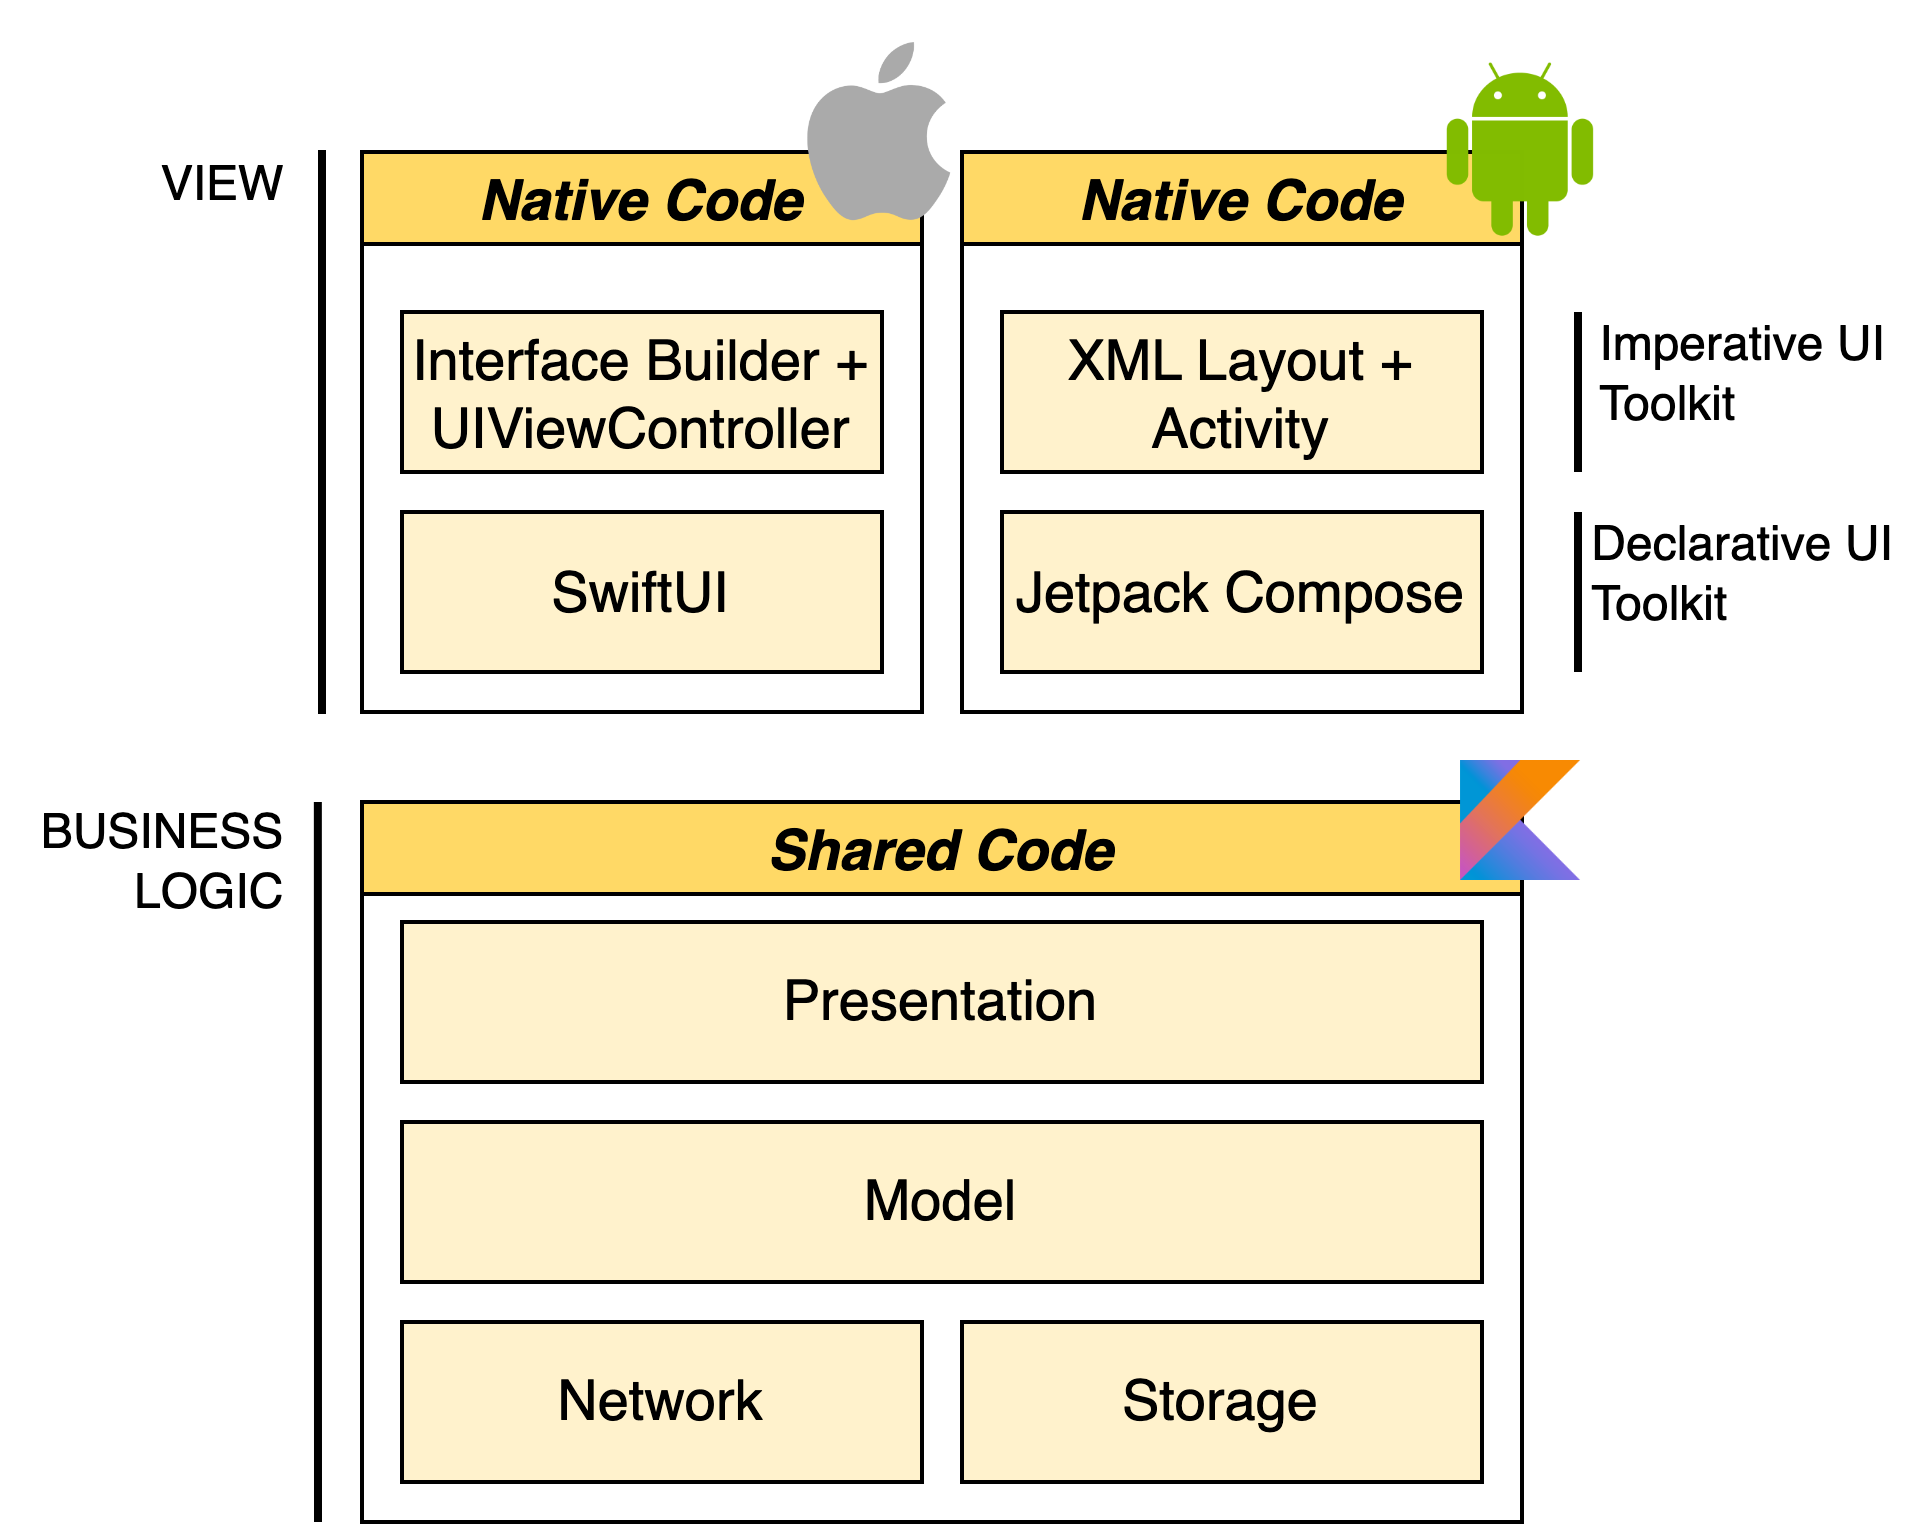
\includegraphics[width=0.7\textwidth]{img/stack_kmm.png}
    \caption{Stack architetturale Kotlin Multiplatform Mobile.}
    \label{stackKMM}
\end{figure}

Con il rilascio di Kotlin 1.7.20 (Settembre 2022), KMM è passato dalla fase \textit{Alpha} alla fase \textit{Beta} la quale è considerata come fase "\textit{pre-stable}"\footnote{\href{https://kotlinlang.org/docs/components-stability.html\#current-stability-of-kotlin-components}{https://kotlinlang.org/docs/components-stability.html\#current-stability-of-kotlin-components}} ma è comunque già stato adottato in produzione per lo sviluppo delle proprie applicazioni mobile da tante aziende tra le quali è possibile trovare nomi rilevanti come Netflix, VMware e Philips\footnote{\href{https://kotlinlang.org/lp/mobile/case-studies/}{https://kotlinlang.org/lp/mobile/case-studies/}}. In base al risultato dell'indagine di mercato svolta nei primi due quadrimestri del 2021\footnote{\href{https://blog.jetbrains.com/kotlin/2021/10/multiplatform-survey-q1-q2-2021/}{https://blog.jetbrains.com/kotlin/2021/10/multiplatform-survey-q1-q2-2021/}}, le porzioni di codice condiviso nelle applicazioni sviluppate con KMM sono: 85\% networking, 75\% data storage, 70\% utilities, $\sim$60\% algoritmi/computazione, $\sim$55\% state management e $\sim$50\% presenters/controllers/view models.

KMM consiste in un caso d'uso specifico (e il più diffuso) del framework Kotlin MultiPlatform (KMP), il quale permette di sviluppare il codice in modo agnostico rispetto le piattaforme target e di condividerlo tra differenti piattaforme. Il framework KMM è fortemente basato sui seguenti compilatori inclusi nell'ecosistema Kotlin~\cite{nagy2022simplifying}:

\begin{itemize}
    \item \textbf{Kotlin/JVM} - Utilizzato per la piattaforma Android, permette di compilare codice Kotlin in bytecode Java (\textit{.class}), il quale può essere eseguito direttamente sulla JVM. Nel caso di Android è necessario un ulteriore passaggio per tradurre il bytecode Java in bytecode Dalvik (\textit{.dex}).

    \begin{figure}[H]
        \centering
        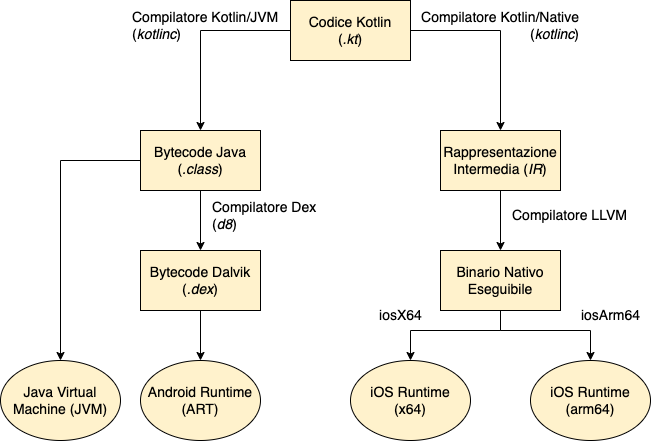
\includegraphics[width=0.8\textwidth]{img/compilatore_kotlin.png}
        \caption{Fasi di compilazione Kotlin/JVM e Kotlin/Native.}
    \end{figure}

    \item \textbf{Kotlin/Native} - Utilizzato per la piattaforma iOS. A differenza del compilatore Kotlin/JVM, il compilatore Kotlin/Native è progettato per quelle situazioni dove non è possibile o non si vuole avere una VM come nel caso dei dispositivi embedded e della piattaforma iOS. Per fare ciò include un backend basato su \textit{Low Level Virtual Machine} (LLVM)\footnote{\href{https://llvm.org/}{https://llvm.org/}} in grado di compilare il codice Kotlin in binari nativi che possono essere eseguiti senza VM\cite{nagy2022simplifying}. Le piattaforme supportate da Kotlin/Native attualmente sono macOS, iOS, tvOS, watchOS, Linux, Windows (MinGW) e Android NDK\footnote{\href{https://kotlinlang.org/docs/native-overview.html\#target-platforms}{https://kotlinlang.org/docs/native-overview.html\#target-platforms}} e per ognuna di esse esistono differenti architetture. Nel caso di iOS le differenti architetture supportate da KMM sono \textit{Arm64}, \textit{Arm32} e \textit{x64}. Anche in questo caso sono necessarie due fasi di compilazione: (\textit{i}) il codice Kotlin viene compilato nella \textit{Rappresentazione Intermedia} (IR) LLVM e (\textit{ii}) successivamente compilato nel binario nativo.
\end{itemize}

\subsubsection{Struttura Applicazione KMM}
Una applicazione sviluppata con KMM segue lo stack definito dalla condivisione della business logic e la separazione della UX/UI (figura \ref{stackKMM}). Il modulo \textit{shared} contiene tutta la business logic condivisa, la quale può essere sviluppata tramite l'utilizzo di librerie con supporto nativo al framework KMM, cioè librerie che forniscono già al loro interno specifiche implementazioni per le diverse piattaforme target, oppure tramite l'utilizzo del meccanismo expect/actual.

\begin{figure}[H]
    \centering
    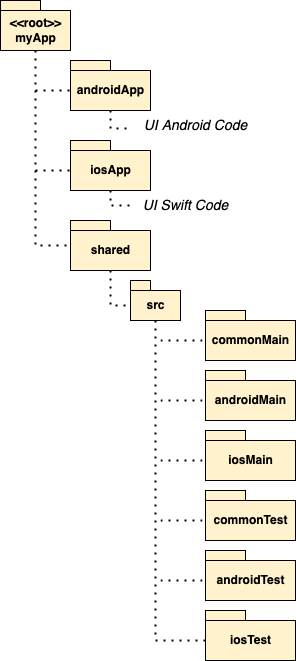
\includegraphics[width=0.5\textwidth]{img/struttura_app_kmm.png}
    \caption{Struttura dei moduli di una applicazione KMM.}
\end{figure}

Nel caso di utilizzo del meccanismo expect/actual è necessario definire le funzionalità nel modulo \textit{commonMain} e fornire le implementazioni per le specifiche piattaforme nei relativi moduli \textit{androidMain} e \textit{iosMain}. Gli stessi concetti vengono applicati per la struttura dei moduli di test: \textit{commonTest}, \textit{androidTest} e \textit{iosTest}.

I moduli UX/UI delle relative piattaforme includono il codice condiviso come dipendenza di progetto, in particolare come dipendenza Gradle (\textit{aar}\footnote{Android Archive}) per Android e come dipendenza CocoaPods (Pod) per iOS.

\subsubsection{Expect/Actual}
Quando si sviluppa codice condiviso è spesso necessario definire come determinate funzionalità debbano essere implementate sulla specifica piattaforma target per utilizzare i relativi SDK. Il framework KMM fornisce il meccanismo \textit{expect/actual} per assolvere a questo compito in modo del tutto analogo al design pattern \textit{Template Method}:
\begin{itemize}
    \item \textbf{Expect} - Astrazione della funzionalità necessaria. Tramite la keywork \textit{expect} si definisce lo scheletro astraendo dalla specifica implementazione.
    \item \textbf{Actual} - Implementazione specifica per una determinata piattaforma. Tramite la keywork \textit{actual} si definisce l'implementazione, reificando l'astrazione definita tramite il concetto di \textit{expect}.
\end{itemize}

Il seguente codice\footnote{\href{https://github.com/paganellif/DevOps-per-applicazioni-mobile-un-caso-di-studio-industriale/tree/3-applicazioni-multipiattaforma/kmm-example/shared}{https://github.com/paganellif/DevOps-per-applicazioni-mobile-un-caso-di-studio-industriale/tree/3-applicazioni-multipiattaforma/kmm-example/shared}} mostra un esempio elementare di utilizzo del meccanismo:

\begin{listing}[H]
    \inputminted{kotlin}{code/3-expectactual}
    \caption{Esempio di applicazione expect/actual per ottenere informazioni sulla piattaforma.}
\end{listing}

I seguenti screenshot, catturati tramite l'esecuzione degli appositi emulatori delle piattaforme target, mostrano l'efficacia del meccanismo expect/actual: l'applicazione è stata compilata utilizzando le differenti implementazioni in modo corretto.

\begin{multicols}{2}
    \begin{figure}[H]
        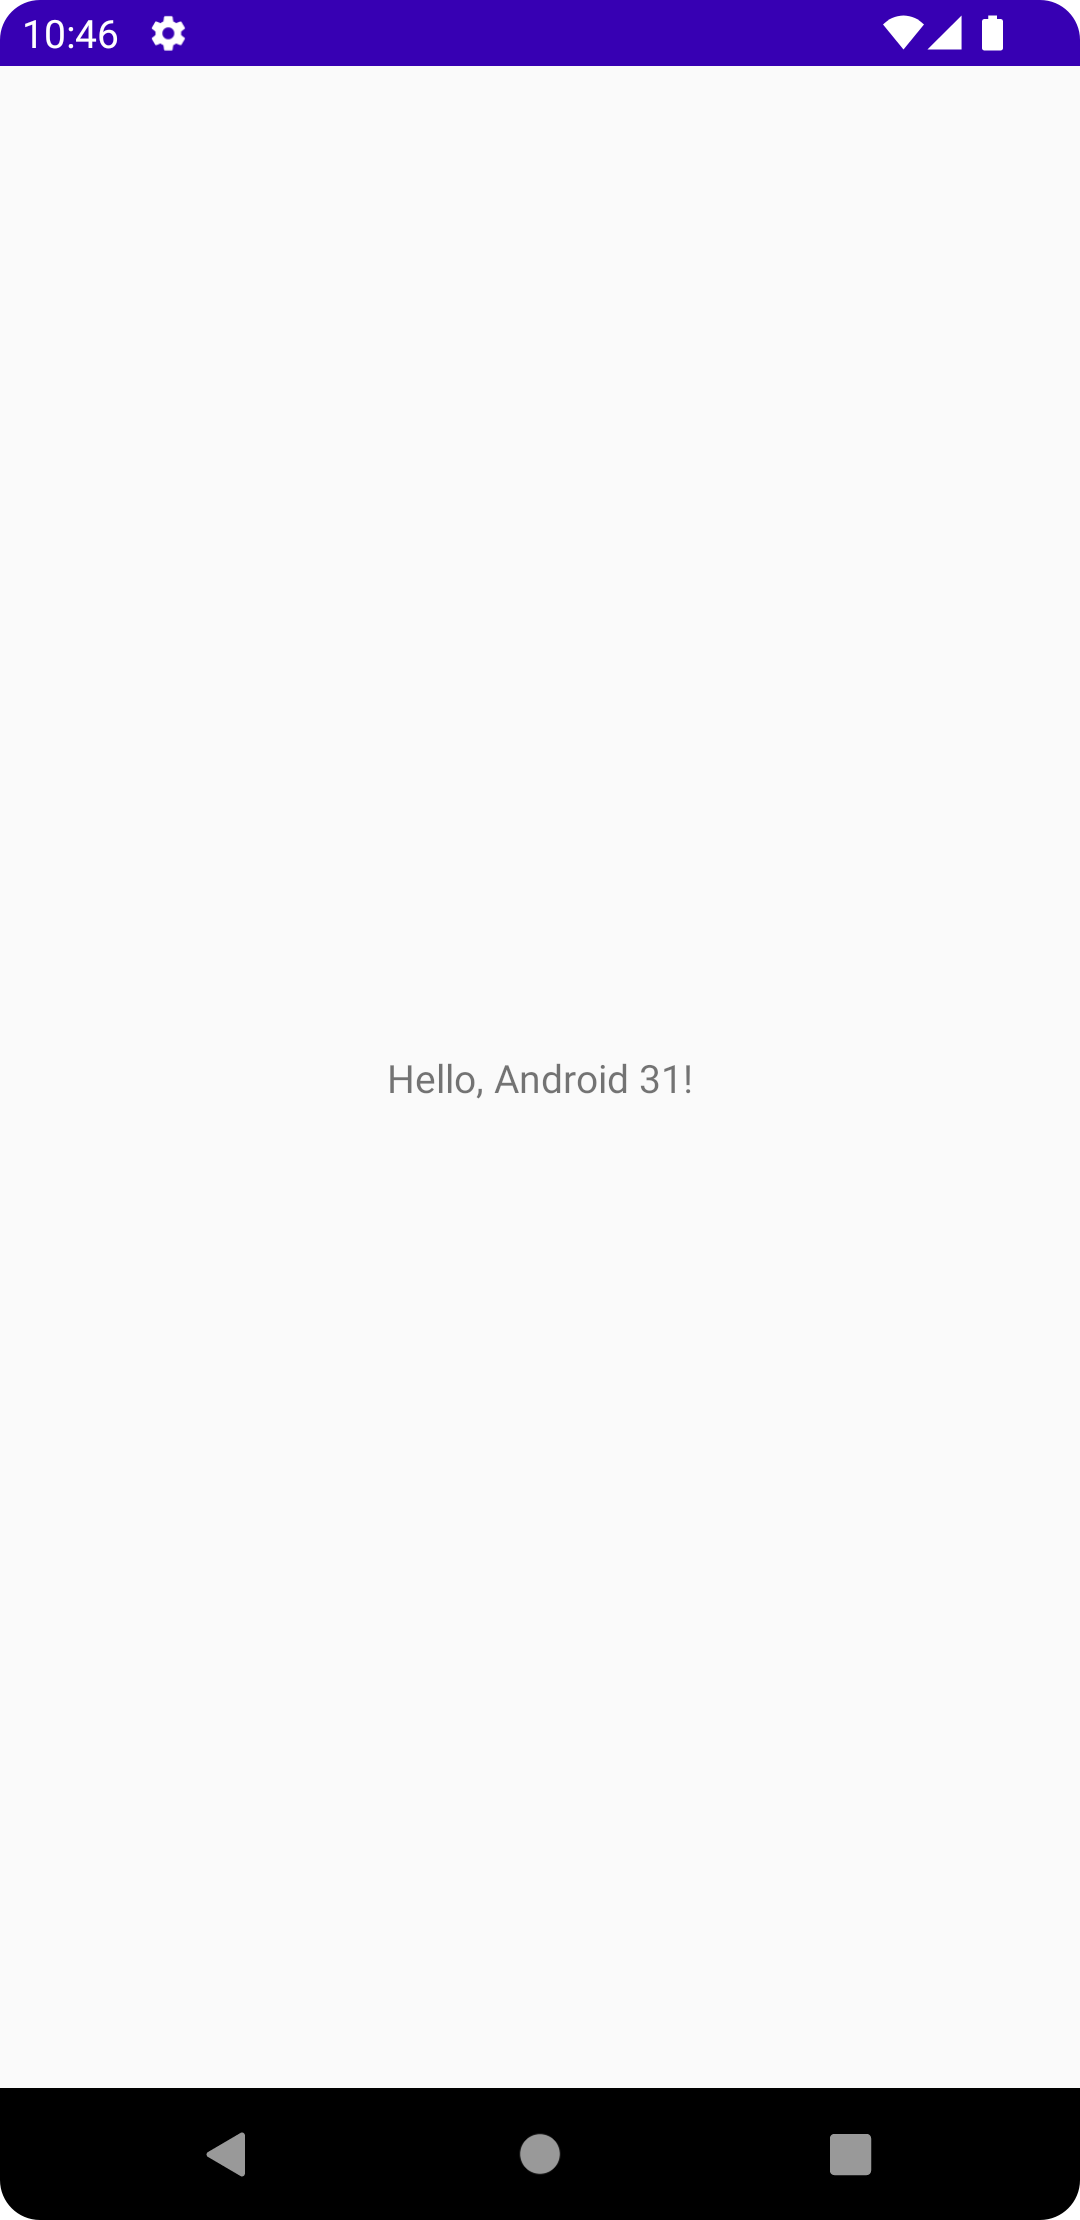
\includegraphics[width=0.37\textwidth]{img/kmm_example_android.png}
        \caption{Esempio expect/actual in esecuzione sulla piattaforma Android}
        \label{expect-actual-android}
    \end{figure}

    \begin{figure}[H]
        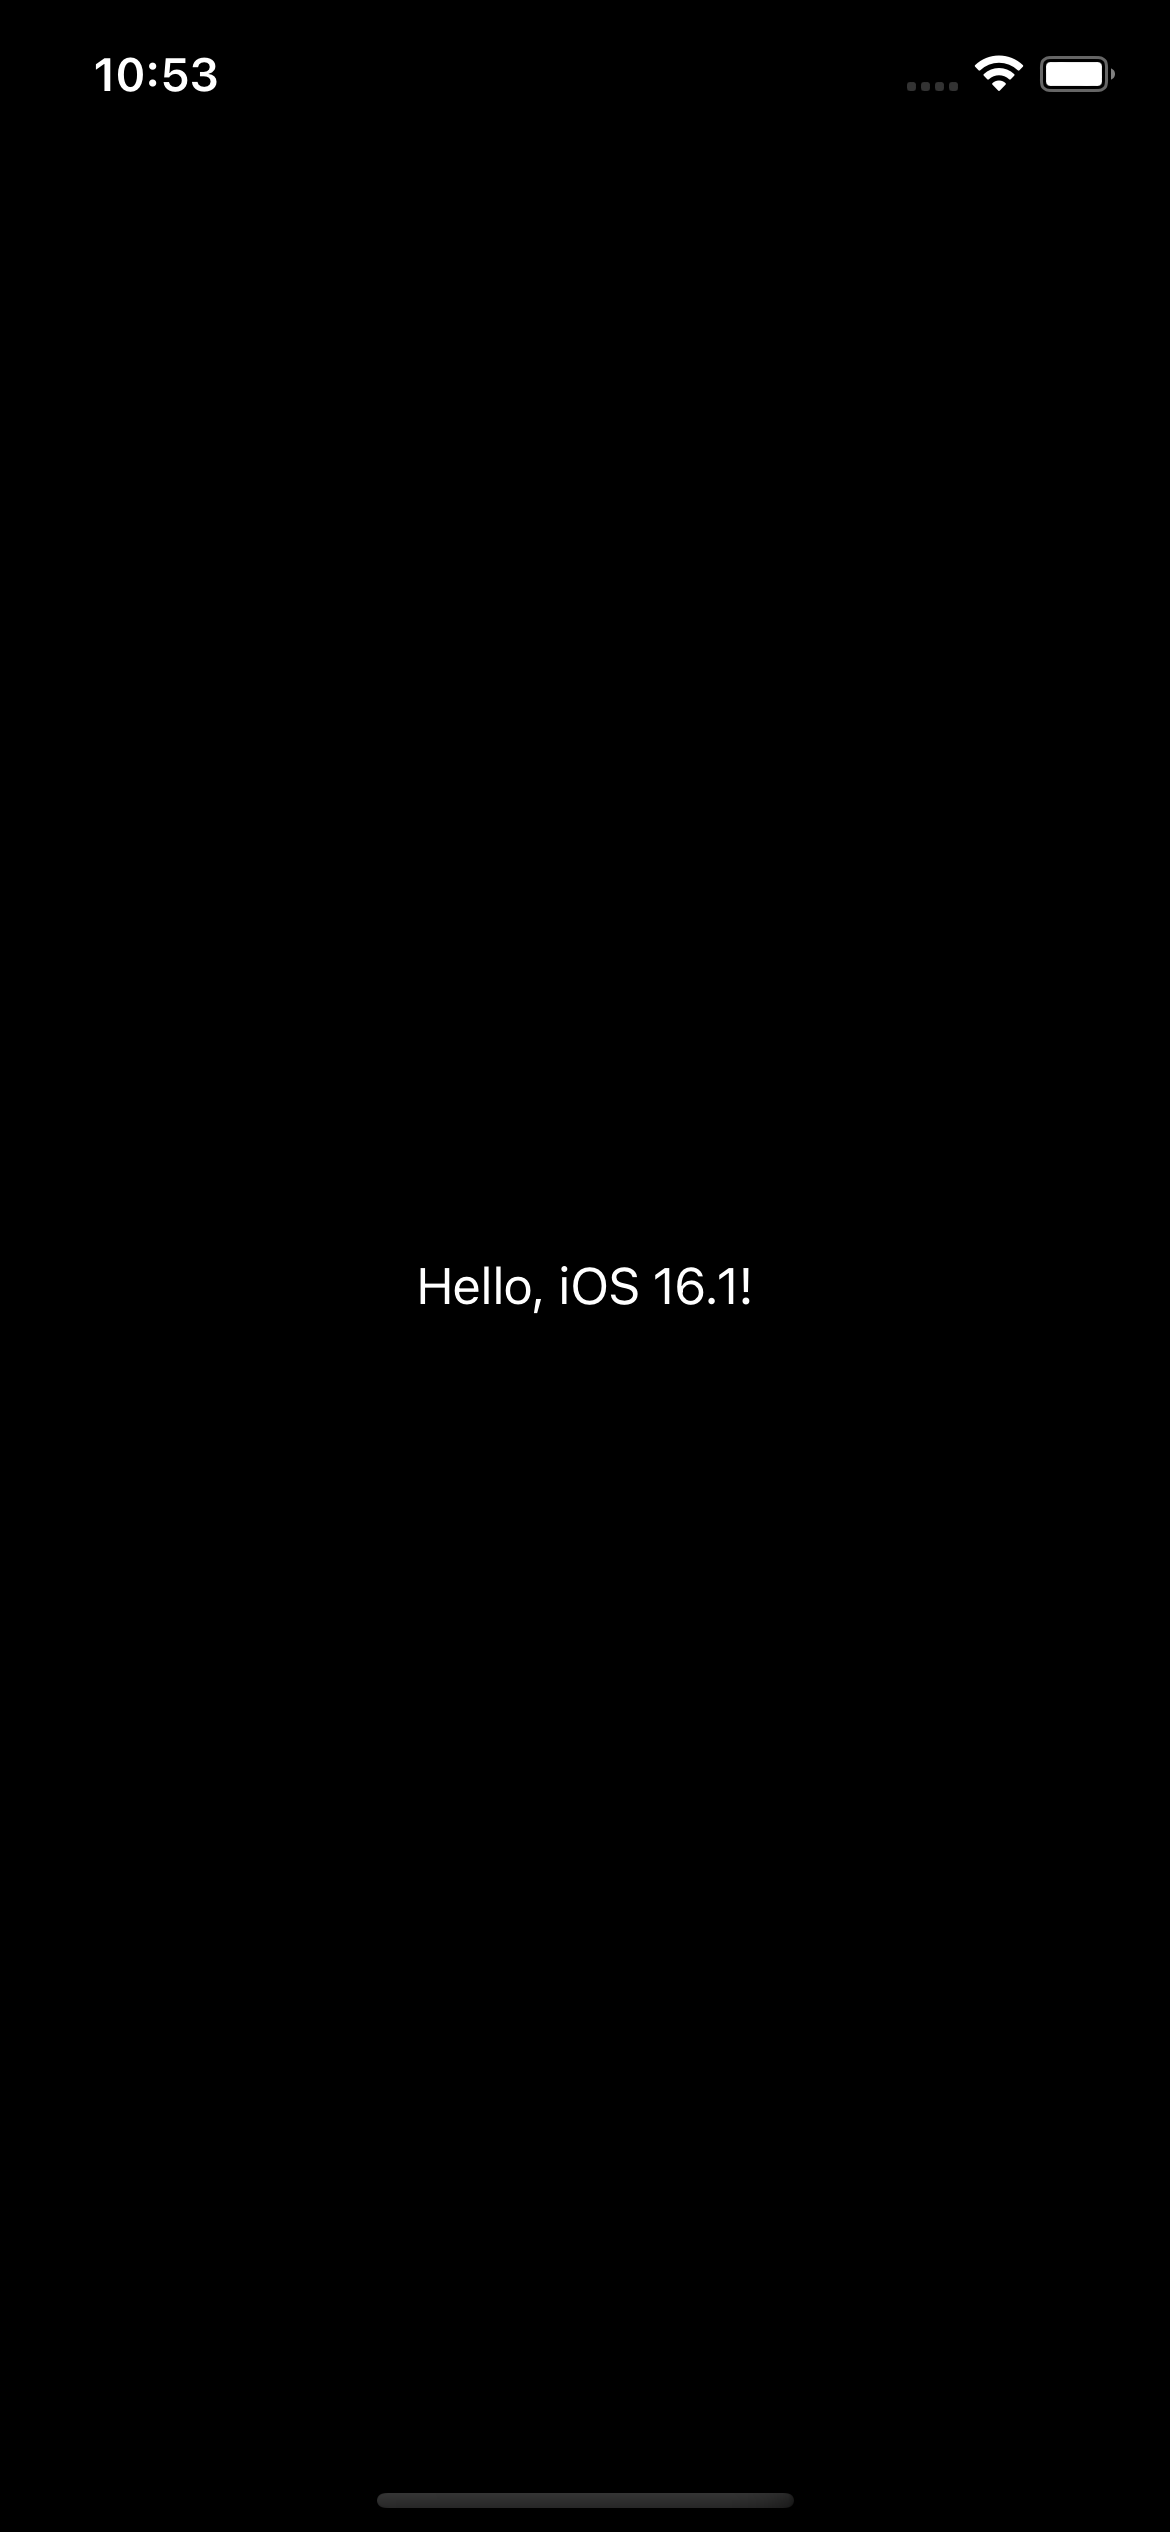
\includegraphics[width=0.35\textwidth]{img/kmm_example_ios_dark.png}
        \caption{Esempio expect/actual in esecuzione sulla piattaforma iOS}
        \label{expect-actual-ios}
    \end{figure}
\end{multicols}

\subsubsection{KMM Gradle Plugins}
Gli strumenti di build automation permettono la gestione di tutti quei task riguardanti la compilazione del codice. Gradle rappresenta il tool di build automation ufficiale Android ed è possibile sviluppare delle estensioni, chiamate plugins, per aggiungere task custom allo strumento. E' proprio tramite questo meccanismo che KMM permette l'esecuzione dei task relativi allo sviluppo di applicazioni mobile multiplatform.

Il plugin Gradle KMM fornisce uno specifico DSL\footnote{Domain Specific Language} per definire e configurare i task necessari a compilare il codice condiviso per le relative piattaforme target\footnote{\href{https://kotlinlang.org/docs/multiplatform-dsl-reference.html}{https://kotlinlang.org/docs/multiplatform-dsl-reference.html}}. Alcune delle principali tipologie di task sono:

\begin{itemize}
    \item \textbf{Build} - tasks per build, compile, link
    \item \textbf{CocoaPods} - tasks per la gestione delle dipendenze Swift/Objective-C
    \item \textbf{Interop} - tasks relativi all'utilizzo del \textit{commonizer}\footnote{\href{https://github.com/JetBrains/kotlin/tree/master/native/commonizer}{https://github.com/JetBrains/kotlin/tree/master/native/commonizer}}
    \item \textbf{Verification tasks} - tasks per l'esecuzione dei test
\end{itemize}

Lo strumento di build automation Gradle e i relativi plugins utilizzati vengono configurati tramite specifici file locati insieme ai sorgenti del progetto. Il seguente codice\footnote{\href{https://github.com/paganellif/DevOps-per-applicazioni-mobile-un-caso-di-studio-industriale/blob/3-applicazioni-multipiattaforma/kmm-example/shared/build.gradle.kts}{https://github.com/paganellif/DevOps-per-applicazioni-mobile-un-caso-di-studio-industriale/blob/3-applicazioni-multipiattaforma/kmm-example/shared/build.gradle.kts}} mostra come è possibile configurare il modulo condiviso tramite l'apposito DSL. E' in questo file di configurazione che si definiscono le specifiche dipendenze e task per le piattaforme target:

\begin{listing}[H]
\inputminted{kotlin}{code/3-gradlekmm2}
\caption{Definizione utilizzo Plugin Gradle KMM nel file \textit{build.gradle.kts} del modulo condiviso (Kotlin).}
\end{listing}

\subsection{Fastlane}
Nonostante vi sia la necessità di utilizzare diversi strumenti di build automation per l'esecuzione dei task di sviluppo per le due differenti piattaforme Android e iOS, il processo di sviluppo e le fasi che lo compongono sono comuni, indipendentemente dalla piattaforma target. Come descritto nei capitoli precedenti, lo sviluppatore deve essere in grado non solo di eseguire task strettamente correlati alla fase di sviluppo ma anche di eseguire tutti quei task che riguardano il testing, la stabilizzazione e il rilascio di una applicazione.

Tra gli strumenti open-source dedicati allo sviluppo di applicazioni multipiattaforma uno dei più popolari è sicuramente Fastlane\footnote{\href{7https://github.com/fastlane/fastlane}{7https://github.com/fastlane/fastlane}}. Il punto di forza di questo tool è il supporto a tutte le fasi del processo di sviluppo di applicazioni mobile per entrambe le piattaforme Android e iOS mettendo lo sviluppatore nella condizione di poter operare su tutto il processo tramite un unico tool.

I task del delle varie fasi del processo definiscono il comportamento di Fastlane e devono essere descritti negli appositi file di configurazione Fastfile e Appfile utilizzando due concetti principali:

\begin{itemize}
    \item \textbf{Action} - Elaborazione pre-definita e configurabile tramite passaggio di parametri, rappresenta il task che deve essere eseguito.
    \item \textbf{Lane} - Insieme di action definito dall'utente per descrivere elaborazioni complesse, ovvero task composti da più sotto-task.
\end{itemize}

Il seguente codice\footnote{\href{https://github.com/paganellif/DevOps-per-applicazioni-mobile-un-caso-di-studio-industriale/blob/3-applicazioni-multipiattaforma/fastlane/fastlane/Fastfile}{https://github.com/paganellif/DevOps-per-applicazioni-mobile-un-caso-di-studio-industriale/blob/3-applicazioni-multipiattaforma/fastlane/fastlane/Fastfile}} rappresenta un esempio di lane Fastlane per il rilascio in versione beta di applicazioni iOS. Tale lane, chiamata \textit{beta}, è composta da quattro action rispettivamente per: (\textit{i}) inizializzare l'ambiente per connettersi ai servizi cloud Apple e scaricare tutto il necessario per la fase di firma del codice, (\textit{ii}) compilazione del codice Swift e creazione del pacchetto \textit{ipa} contenente l'applicazione iOS, (\textit{iii}) pubblicazione in versione beta su Testflight e (\textit{iv}) invio della notifica dell'avvenuta pubblicazione su un canale Slack dedicato.

\begin{listing}[H]
    \inputminted{ruby}{code/4-fastlane}
    \caption{Esempio di definizione di una lane Fastlane per il rilascio in versione beta di applicazioni iOS}
\end{listing}

\chapter{Metodologia DevOps}
\label{ch:ch2}
% !TeX root = ../main.tex

\section{Introduzione}
% cos'è devops, la filosofia devops, no silos, ecc

\section{Tecniche di automazione e vantaggi}
\subsection{Continuous Integration}

\subsection{Continuous Delivery}

\subsection{Continuous Inspection}

\section{Strumenti}
% descrizione strumenti per l'automazione in generale (gitlab runner + Pipeline as Code)
\subsection{Pipeline as Code}

\subsection{Runners}

\subsection{Software as a Service}
% descrizione strumenti as a service per l'automazione del processo (runner managed, sonarcloud, ...) e dello dello sviluppo mobile (xcode cloud, bitrise, google play console, testflight)

\chapter{Caso di studio: applicazione MaggioliEbook}
\label{ch:ch3}
% !TeX root = ../main.tex

\section{Introduzione}
In questo capitolo vengono inizialmente descritte le motivazioni che hanno spinto l'azienda Maggioli S.p.A.\footnote{\href{https://www.maggioli.com/en-us}{https://www.maggioli.com/en-us}} a dedicare risorse per la ricerca e la sperimentazione nei campi delle applicazioni multipiattaforma e delle tecniche DevOps in ambito mobile.
Successivamente sono indicati i requisiti del caso di studio industriale individuato, 
il quale può essere suddiviso in due macroaree:

\begin{itemize}
    \item definizione del processo di sviluppo per applicazioni multipiattaforma tramite l'adozione della cultura DevOps,
    
    \item sviluppo di un'applicazione mobile multipiattaforma utilizzando il processo di sviluppo definito.
\end{itemize}

\section{Contesto aziendale}
Tra i core business dell'azienda Maggioli S.p.A. è rimasto centrale il ruolo dell'editoria,
ma col trascorrere degli anni e il mutare delle esigenze dei clienti, 
i quali sono principalmente pubblica amministrazione (PA) e professionisti privati, 
come avvocati, 
architetti, 
commercialisti ed ingegneri edili, 
si è verificata una transizione verso il mondo digitale.

I servizi digitali erogati per la consultazione delle pubblicazioni hanno superato considerevolmente il formato cartaceo,
il quale rimane comunque un metodo secondario di consultazione disponibile seppur in forma molto ridotta. 
Per l'editoria digitale esiste in Maggioli una business unit dedicata, 
chiamata \textit{Digital Media}, 
il cui ruolo principale consiste nella realizzazione e manutenzione dei siti Web Maggioli dedicati alla ricerca e visualizzazione delle pubblicazioni digitali. 
I seguenti sono soltanto alcuni dei siti gestiti dal team \textit{Digital Media}: 
Biblioteca Digitale\footnote{\href{https://bibliotecadigitale.maggioli.it/}{https://bibliotecadigitale.maggioli.it/}}, 
Appalti \& Contratti\footnote{\href{https://www.appaltiecontratti.it/}{https://www.appaltiecontratti.it/}} e Periodici\footnote{\href{https://www.periodicimaggioli.it/}{https://www.periodicimaggioli.it/}}. 
La necessità principale è dunque quella di fare innovazione tramite lo sviluppo di un'applicazione mobile in modo da fornire ai clienti Maggioli un nuovo metodo di accesso alle pubblicazioni che sia più accessibile e comodo.

\begin{figure}[H]
    \centering
    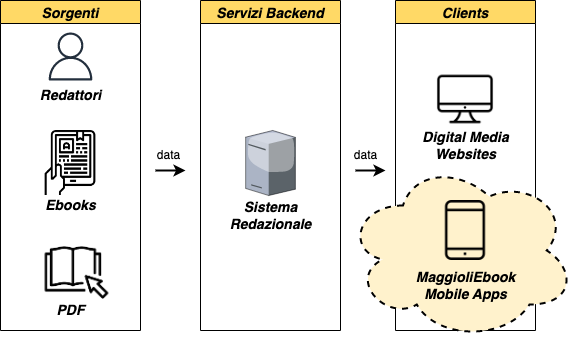
\includegraphics[width=0.75\textwidth]{img/contesto-aziendale.png}
    \caption{Schema del contesto aziendale in cui è collocato il caso di studio}
    \label{contesto-aziendale-fig}
\end{figure}

Le motivazioni che stanno alla base della scelta della cultura DevOps e delle applicazioni multipiattaforma per lo sviluppo di questo caso di studio sono comuni a qualsiasi tipologia d'azienda: 
come descritto nei capitoli \ref{ch:devops} e \ref{ch:app-multiplatform} è possibile ottimizzare il processo di sviluppo diminuendo le risorse impiegate e quindi i costi ma allo stesso tempo aumentando la qualità del software e la frequenza di rilascio,
i quali comportano una maggiore soddisfazione sia da parte dell'utente finale che da parte dell'azienda.

\section{Definizione processo di sviluppo}
Considerando l'intero contesto aziendale esistono degli standard, 
consolidati con l'esperienza maturata nello sviluppo software, 
che devono essere adottati sia per quanto riguarda il processo di sviluppo che la scelta degli strumenti necessari. 
L'obiettivo è riuscire a definire un modello di processo fortemente basato sugli standard aziendali ma adattato alle esigenze dello sviluppo di applicazioni mobile multipiattaforma e che possa essere introdotto nei team che si occupano di applicazioni mobile. 
I principali standard aziendali riguardanti gli strumenti e le tecnologie che devono essere adottati sono:

\begin{itemize}
    \item \textbf{GitLab}\footnote{\href{https://about.gitlab.com/}{https://about.gitlab.com/}} (\textit{DVCS/CI Server}) - Le funzionalità necessarie al versionamento del codice, alla collaborazione/pianificazione e all'automazione (Sezione \ref{devops-tools-sec}) sono tutte soddisfatte dalla piattaforma cloud GitLab con la quale è presente una sottoscrizione di piano di licenza aziendale.
    
    \item \textbf{SonarQube}\footnote{\href{https://www.sonarqube.org/}{https://www.sonarqube.org/}} (\textit{Vulnerability Management System}) - Questo servizio self-hosted è reso disponibile a tutti i team aziendali e permette di soddisfare gran parte dei task di Continuous Inspection. Grazie a SonarQube è possibile effettuare l'analisi statica del codice, validare il rispetto di determinate policy aziendali e visualizzare dashboard sullo stato delle scansioni.
    
    \item \textbf{Renovate}\footnote{\href{https://docs.renovatebot.com/}{https://docs.renovatebot.com/}} (\textit{Dependency Management}) - Strumento utilizzato per automatizzare la gestione delle dipendenze dei progetti. 
\end{itemize}

La pipeline standard a livello aziendale, 
base di partenza per la definizione della pipeline per applicazioni mobile multipiattaforma, 
rispetta a pieno tutte le considerazioni fatte nel capitolo \ref{ch:devops} per tutte le tecniche d'automazione indicate (fig. \ref{ci-inspection-pipeline}). 
Tramite l'adattamento delle fasi di integration, delivery e inspection di questa pipeline con le necessità dello sviluppo mobile indicate nei capitoli \ref{ch:sdlc} e \ref{ch:app-multiplatform} si ottengono i seguenti requisiti e dunque la pipeline obiettivo da realizzare.

\subsection{Requisiti}
\begin{itemize}
    \item \textbf{R1} - Continuous Integration
    \begin{itemize}
        \item \textbf{R1.1} - Stage di compilazione, testing e packaging con i relativi sotto-task per entrambe le piattaforme Android e iOS.
        
        \item \textbf{R1.2} - L'output dell'ultimo stage deve essere un pacchetto contenente l'applicazione da passare come artefatto alla fase successiva di delivery.
        
        \item \textbf{R1.3} - Utilizzo del sistema aziendale di gestione automatica delle dipendenze Renovate.
    \end{itemize}
    
    \item \textbf{R2} - Continuous Delivery
    \begin{itemize}
        \item \textbf{R2.1} - Stage di stabilizzazione suddivisi tra \textit{Alpha} e \textit{Beta} per il testing interno ed esterno tramite gli appositi servizi forniti da Google e Apple: Google Play Console per l'applicazione Android e Testflight per l'applicazione iOS.
        
        \item \textbf{R2.2} - L'applicazione soggetta a stabilizzazione è data in input dalla fase precedente di integrazione.
        
        \item \textbf{R2.3} - Stage di pubblicazione sui relativi marketplace Google Play Store o App Store. L'applicazione soggetta a pubblicazione deriva dalla terminazione con successo della fase di stabilizzazione e si trova già sui portali utilizzati.
    \end{itemize}
    
    \item \textbf{R3} - Continuous Inspection
    \begin{itemize}
        \item \textbf{R3.1} - Stage di analisi statica e analisi delle dipendenze per entrambe le piattaforme.
        
        \item \textbf{R3.2} - Utilizzo del sistema aziendale di gestione delle vulnerabilità centralizzato SonarQube.
    \end{itemize}
    
    \item \textbf{R4} - Tutto il sistema di automazione deve poter essere utilizzato da altri team di sviluppo all'interno dell'azienda.
\end{itemize}

\begin{figure}[H]
    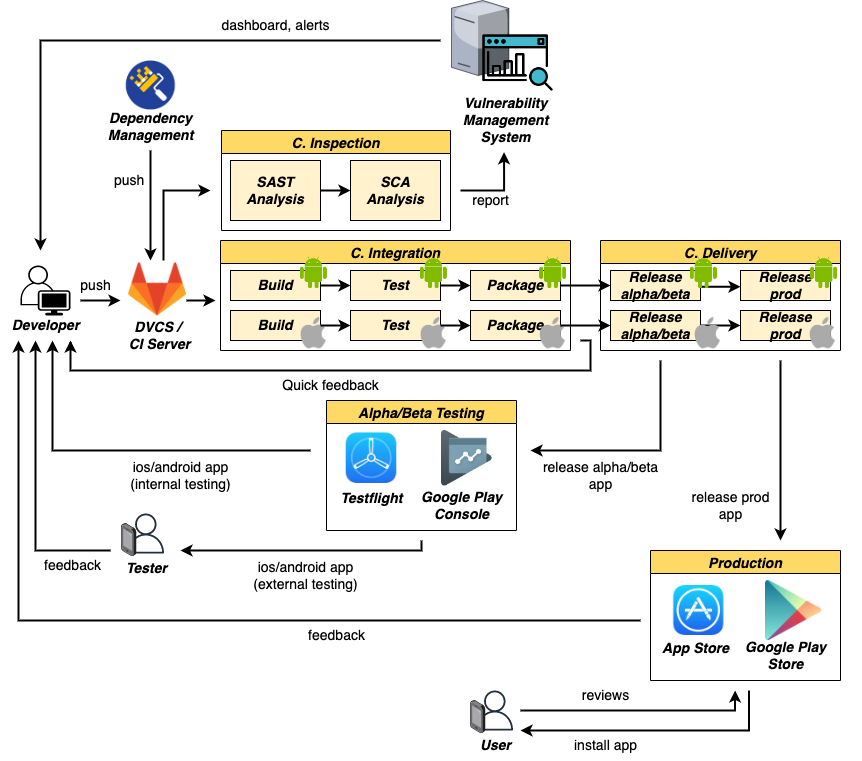
\includegraphics[width=1\textwidth]{img/full-cicd.png}
    \caption{Schema globale del processo di sviluppo automatizzato che si intende realizzare}
    \label{full-cicd}
\end{figure}

\section{Definizione applicazione}
Dato il contesto aziendale dell'editoria digitale in cui si colloca il caso di studio,
è possibile catalogare l'applicazione mobile da sviluppare come \textit{E-Reader}. 
Un e-book reader, 
chiamato anche e-book device o e-reader, 
è un dispositivo elettronico mobile progettato principalmente per la lettura di e-book e periodici digitali. 
Ogni dispositivo in grado di mostrare del testo su uno schermo potrebbe essere considerato un e-reader, 
ma i dispositivi progettati appositamente per questo compito hanno caratteristiche e funzionalità specifiche come l'ottimizzazione della portabilità, 
la leggibilità e la durata della batteria~\cite{shoba2014vocabulary}.

Per poter avere un valore aggiunto rispetto alle funzionalità già fornite dai siti Web sviluppati dal team \textit{Digital Media},
l'applicazione ``MaggioliEbook'' deve comportarsi come un vero e proprio e-reader, 
integrandosi ai servizi backend Maggioli per l'editoria digitale già esistenti. 
Data la complessità del dominio da modellare sono stati svolti degli incontri con figure interne esperte di dominio appartenenti ai team \textit{Ricerca e Sviluppo} e \textit{Digital Media}, 
al fine di definire (\textit{i}) terminologia, 
(\textit{ii}) casi d'uso e (\textit{iii}) requisiti.

\subsection{Terminologia e casi d'uso}
E' necessario che il team di sviluppo, 
composto da figure tecniche, 
e i committenti, 
i quali sono invece esperti interni di dominio, 
utilizzino lo stesso linguaggio per far si che le successive fasi del processo siano efficaci ed efficienti. 

Il concetto di \textit{Ubiquitous Language} definisce un vocabolario condiviso da entrambe le parti per la discussione del software~\cite{evans_domain-driven_2004} ed è stato adottato per la realizzazione del seguente glossario, 
il quale racchiude tutti i principali termini utilizzati negli incontri tra team di sviluppo ed esperti di dominio, 
suddivisi in \textit{entità} e \textit{casi d'uso}:

\subsubsection*{Entità}
\begin{table}[H]
\centering
    \begin{tabular}{|c|c|}
         \hline
         \textbf{Termine} & \textbf{Descrizione}\\
         \hline
         \textit{Reader} & \specialcell{Lettore di documenti in grado di visualizzarli ed \\interagire con essi.}\\
         \hline
         \textit{Documento} & Contenuto digitale pubblicato da Maggioli Editore.\\
         \hline
         \textit{Documento Statico} & Documento con una certa struttura definita (PDF).\\
         \hline
         \textit{Documento Fluido} & \specialcell{Documento senza struttura in grado di adattarsi al dispositivo\\ in cui viene aperto (EPUB).}\\
         \hline
         \textit{Libro} & \specialcell{Tipologia principale di documento fluido fruibile\\ tramite l'applicazione MaggioliEbook.}\\
         \hline
         \textit{Rivista} & \specialcell{Tipologia principale di documento statico fruibile\\ tramite l'applicazione MaggioliEbook.}\\
         \hline
         \textit{Bookmark} & Identifica una specifica pagina di un libro o di una rivista.\\
         \hline
         \textit{Progression} & \specialcell{Progresso di lettura di un libro o di una rivista,\\ calcolato in percentuale \\(numero di pagine lette sul totale del documento).}\\
         \hline
         \textit{Highlight} & \specialcell{Annotazione per una certa porzione testuale di \\documento. Può essere una evidenziazione, sottolineatura \\o annotazione testuale.}\\
         \hline
         \textit{Favorite} &  Documento preferito dall'utente.\\
         \hline
         \textit{User} & Utente con uno o più abbonamenti attivi.\\
         \hline
          \textit{Token} & \specialcell{Autentica e autorizza l'utente ad accedere ai vari documenti\\ per i quali esiste un abbonamento attivo.}\\
         \hline
    \end{tabular}
    \caption{Glossario dei termini (Entità)}
\end{table}

\newpage
\subsubsection*{Casi d'uso}
\begin{table}[H]
\centering
    \begin{tabular}{|c|c|}
         \hline
         \textbf{Termine} & \textbf{Descrizione}\\
         \hline
         \textit{Apertura Documento} & \specialcell{Richiesta di apertura in lettura di uno specifico\\ documento.}\\
         \hline
         \textit{Chiusura Documento} & Richiesta di chiusura del documento aperto in lettura.\\
         \hline
         \textit{Ricerca Documento} & Richiesta di ricerca documento tramite query testuale.\\
         \hline
         \specialcell{\textit{Lettura Metadati}\\\textit{Documento}} & Richiesta di lettura metadati documento.\\
         \hline
         \textit{Creazione Highlight} & Richiesta di creazione annotazioni.\\
         \hline
         \textit{Lettura Highlight} & Richiesta di lettura annotazioni.\\
         \hline
         \textit{Eliminazione Highlight} & Richiesta di eliminazione annotazioni.\\
         \hline
         \textit{Creazione Bookmark} & Richiesta di creazione segnalibri.\\
         \hline
         \textit{Lettura Bookmark} & Richiesta di lettura segnalibri.\\
         \hline
         \textit{Eliminazione Bookmark} & Richiesta di eliminazione segnalibri.\\
         \hline
         \textit{Creazione Progression} & \specialcell{Richiesta di salvataggio dell'\\avanzamento di lettura di un documento.}\\
         \hline
         \textit{Lettura Progression} &  \specialcell{Richiesta di lettura dell'\\avanzamento di lettura di un documento.}\\
         \hline
         \textit{Eliminazione Progression} &  \specialcell{Richiesta di eliminazione dell'\\avanzamento di lettura di un documento.}\\
         \hline
         \textit{Creazione Favorite} &  Richiesta di creazione preferiti.\\
         \hline
         \textit{Lettura Favorite} & Richiesta di lettura preferiti.\\
         \hline
         \textit{Eliminazione Favorite} & Richiesta di eliminazione preferiti.\\
         \hline
         \specialcell{\textit{Conversione}\\\textit{PDF2EPUB}} & \specialcell{Richiesta di conversione di un documento statico in\\ documento fluido (dal formato PDF al formato EPUB).}\\
         \hline
         \specialcell{\textit{Download Contenuto}\\\textit{Documenti}} & Scaricamento del contenuto dei documenti.\\
         \hline
         \specialcell{\textit{Download Copertina}\\\textit{Documenti}} & \specialcell{Scaricamento della immagine di copertina dei \\documenti.}\\
         \hline
         \textit{Login User} & Richiesta di login dell'utente (lettura token).\\
         \hline
         \textit{Logout User} & Richiesta di logout dell'utente (eliminazione token).\\
         \hline
         \specialcell{\textit{Controllo Login}\\\textit{User}} & \specialcell{Controllo di autenticazione dell'utente\\ già avvenuta (esistenza token).}\\
         \hline
         \specialcell{\textit{Lettura Account Utente}} & Richiesta informazioni utente (dati anagrafici e mail).\\
         \hline         
    \end{tabular}
    \caption{Glossario dei termini (Casi d'uso)}
\end{table}
\newpage

\begin{figure}[H]
\centering
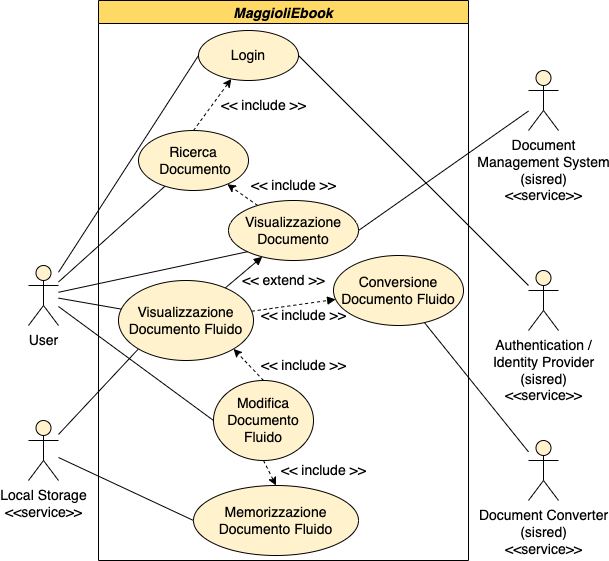
\includegraphics[width=1\textwidth]{img/casi-uso-uml.png}
\caption{UML - Diagramma dei casi d'uso: funzioni/servizi offerti dalla applicazione MaggioliEbook}
\end{figure}

\begin{figure}[H]
\centering
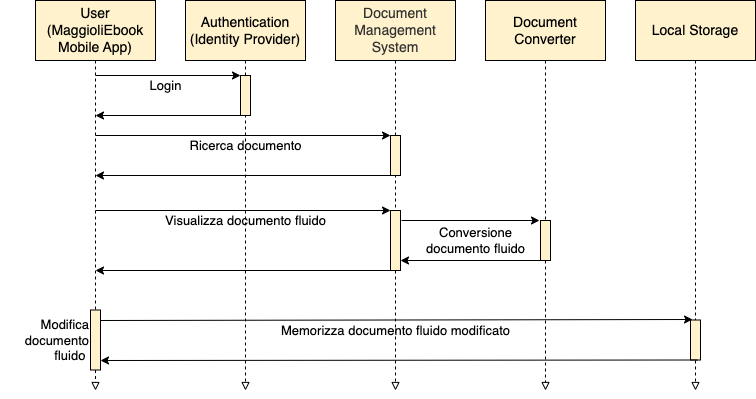
\includegraphics[width=1\textwidth]{img/caso-uso-sequenza-uml.png}
\caption{UML - Diagramma di sequenza: scenario di modifica di un nuovo documento "fluido"}
\end{figure}

\subsection{Requisiti}
\begin{itemize}
    \item \textbf{R1} - Visualizzazione documenti.
    \begin{itemize}
        \item \textbf{R1.1} - In modo fluido, mostrando il contenuto adattato al dispositivo in cui viene mostrato.
        
        \item \textbf{R1.2} - In modo statico, mostrando il contenuto con uno specifico layout indipendente dal dispositivo in cui viene mostrato.
    \end{itemize}
    
    \item \textbf{R2} - Modifica documenti fluidi (lato utente).
    \begin{itemize}
        \item \textbf{R2.1} - Aggiunta segnalibri, commenti, sottolineature, evidenziazioni, al contenuto fluido.
        
        \item \textbf{R2.2} - Memorizzazione segnalibri, commenti, sottolineature, evidenziazioni apportate al contenuto fluido.
    \end{itemize}
    
    \item \textbf{R3} - Gestione utente.
    \begin{itemize}
        \item \textbf{R3.1} - Login (autenticazione) utente.
        
        \item \textbf{R3.2} - Visualizzazione documenti a cui l'utente è abbonato.
    \end{itemize}
    
    \item \textbf{R4} - Ricerca documenti.
    
    \item \textbf{R5} - Conversione documenti da modo statico a modo fluido.
    
    \item \textbf{R6} - Modifica documenti in modo fluido (lato azienda).
    \begin{itemize}
        \item \textbf{R6.1} - Aggiunta elementi/contenuti al documento in modo fluido (hyperlink, quiz, video, immagini, ...).
        
        \item \textbf{R6.2} - Memorizzazione elementi/contenuti aggiunti al documento fluido (hyperlink, quiz, video, immagini, ...).
    \end{itemize}
\end{itemize}

\chapter{Automazione del processo di sviluppo}
\label{ch:ch4}
% !TeX root = ../main.tex

\section{Introduzione}
Nei precedenti capitoli sono stati introdotti i concetti alla base della cultura DevOps, del ciclo di vita del processo di sviluppo di applicazioni mobile e delle applicazioni multipiattaforma, arrivando a definire un caso di studio industriale. In questo capitolo viene descritto come è stato effettivamente realizzato il sistema per l'automazione del processo di sviluppo nel rispetto dei requisiti e delle specifiche indicate nel capitolo precedente.

In questa fase di realizzazione del sistema di automazione e di implementazione della pipeline viene considerato il progetto base\footnote{\href{https://github.com/paganellif/DevOps-per-applicazioni-mobile-un-caso-di-studio-industriale/tree/3-applicazioni-multipiattaforma/kmm-example}{https://github.com/paganellif/DevOps-per-applicazioni-mobile-un-caso-di-studio-industriale/tree/3-applicazioni-multipiattaforma/kmm-example}} fornito dal plugin KMM\footnote{\href{https://plugins.jetbrains.com/plugin/14936-kotlin-multiplatform-mobile}{https://plugins.jetbrains.com/plugin/14936-kotlin-multiplatform-mobile}} per Android Studio al fine di mantenere il focus sul processo in modo più agnostico possibile rispetto ad una specifica applicazione utilizzatrice come può essere MaggioliEbook, argomento trattato nel capitolo successivo.

\section{Self-Hosted MacOS GitLab Runner}
% runner macos: in azienda non esistono runner macos.. riprendere il problema del fatto che apple obbliga a usare macOS, indicare le possibili soluzioni (runner managed/self-hosted, ecc) e come ho configurato il runner self-hosted
% approfondire tipologie di runner executor in gitlab e perche ho usato l'executor shell
Come anticipato nel capitolo \ref{ch:app-multiplatform} tutta la toolchain per lo sviluppo iOS è disponibile solamente per il sistema operativo macOS, il che implica la necessità di un ambiente macOS anche per l'esecuzione della pipeline, almeno per tutti i task riguardanti l'applicazione iOS. Esistono diversi modi per realizzare un sistema di automazione compatibile con i vincoli imposti da Apple e possono essere suddivisi nelle seguenti categorie:

\begin{itemize}
    \item \textbf{Soluzione completa as-a-Service} - Il grande interesse per l'automazione e lo sviluppo di applicazioni iOS da parte delle aziende ha portato alla nascita di servizi cloud completamente dedicati a questo scopo come ad esempio \textit{Bitrise}\footnote{\href{https://www.bitrise.io/home}{https://www.bitrise.io/home}} e \textit{XCode Cloud}\footnote{\href{https://developer.apple.com/xcode-cloud/}{https://developer.apple.com/xcode-cloud/}}.
    \item \textbf{Runner macOS managed} - Come anticipato nel capitolo \ref{ch:devops} un runner, ovvero il componente che esegue effettivamente i task della nostra pipeline, può essere \textit{managed} o \textit{self-hosted}. Nel caso di un runner managed con sistema operativo macOS si evita lo sforzo di configurare e mantenere un componente importante del sistema di automazione ma si hanno costi elevati: solitamente al consumo di risorse di questa tipologia di runner è applicato un fattore moltiplicativo poco sostenibile in termini di costi. Alcuni esempi di piattaforme con questo modello di business per i runner managed sono GitHub Action\footnote{\href{https://docs.github.com/en/billing/managing-billing-for-github-actions/about-billing-for-github-actions\#minute-multipliers}{https://docs.github.com/en/billing/managing-billing-for-github-actions/about-billing-for-github-actions\#minute-multipliers}} e GitLab CI\footnote{\href{https://docs.gitlab.com/ee/ci/pipelines/cicd\_minutes.html\#additional-costs-on-gitlab-saas}{https://docs.gitlab.com/ee/ci/pipelines/cicd\_minutes.html\#additional-costs-on-gitlab-saas}}.
    \item \textbf{Runner macOS self-hosted} - L'altra tipologia di runner consiste nella installazione del componente su una macchina con sistema operativo macOS che deve essere configurata e mantenuta dall'utilizzatore. In questo caso è possibile utilizzare macchine virtuali as-a-Service, come quelle fornite da AWS\footnote{\href{https://aws.amazon.com/ec2/instance-types/mac/}{https://aws.amazon.com/ec2/instance-types/mac/}} (Amazon Web Services), oppure hardware fisico Apple per installare ed eseguire il runner.
\end{itemize}

Data la disponibilità di tutta la toolchain Android per macOS e il costo nullo in caso di runner self-hosted, è stata scelta quest'ultima tipologia per l'esecuzione dell'intera pipeline.

L'installazione e la configurazione di un runner di questa tipologia può essere più o meno complicata in base alle funzionalità necessarie per il sistema di automazione. Nel caso specifico del caso di studio di questo progetto l'unica funzionalità richiesta da configurare è la cache condivisa al fine di abilitare la concorrenza tra più processi e ottimizzare l'esecuzione della pipeline.

I seguenti comandi bash\footnote{\href{https://github.com/paganellif/DevOps-per-applicazioni-mobile-un-caso-di-studio-industriale/blob/5-automazione-del-processo-di-sviluppo/setup-gitlab-macos-runner.sh}{https://github.com/paganellif/DevOps-per-applicazioni-mobile-un-caso-di-studio-industriale/blob/5-automazione-del-processo-di-sviluppo/setup-gitlab-macos-runner.sh}} mostrano la procedura di installazione di un runner GitLab macOS self-hosted su una macchina fisica Apple:
\begin{listing}[H]
    \inputminted{bash}{code/macos-runner-setup.sh}
    \caption{Comandi bash per l'installazione, la configurazione e l'avvio di un runner macOS self-hosted}
\end{listing}

Il seguente codice\footnote{\href{https://github.com/paganellif/DevOps-per-applicazioni-mobile-un-caso-di-studio-industriale/blob/5-automazione-del-processo-di-sviluppo/config.toml}{https://github.com/paganellif/DevOps-per-applicazioni-mobile-un-caso-di-studio-industriale/blob/5-automazione-del-processo-di-sviluppo/config.toml}} mostra il file di configurazione del runner, generato in seguito alla procedura sopra indicata:

\begin{listing}[H]
    \inputminted{toml}{code/macos-runner-config.toml}
    \caption{File di configurazione (\textit{config.toml}) generato al momento della installazione del runner}
\end{listing}

\section{Modello di branching}
L’utilizzo di un adeguato flusso di lavoro è fondamentale per definire una efficiente automazione CI/CD. Con branching si intende l’utilizzo di uno o più flussi principali dai quali divergono altri flussi per svolgere determinati lavori per poi convergere al loro termine: in base alle modalità di apertura e chiusura di questi flussi si definiscono diversi modelli di branching.

Il modello che si intende utilizzare (fig. \ref{branching}) è basato sul modello di branching GitFlow\footnote{\href{https://www.atlassian.com/it/git/tutorials/comparing-workflows/gitflow-workflow}{https://www.atlassian.com/it/git/tutorials/comparing-workflows/gitflow-workflow}} e prevede tre branch principali:

\begin{itemize}
    \item \textbf{dev} - Flusso principale di sviluppo. Ogni modifica apportata a questo branch corrisponde al rilascio di una nuova versione \textit{alpha} per la validazione interna. E' da questo branch che vengono aperti e chiusi nuovi branch, sia per lo sviluppo di nuove funzionalità (\textit{feature}) che per la risoluzione di bug/patch (\textit{fix}).

    \begin{figure}[H]
        \centering
        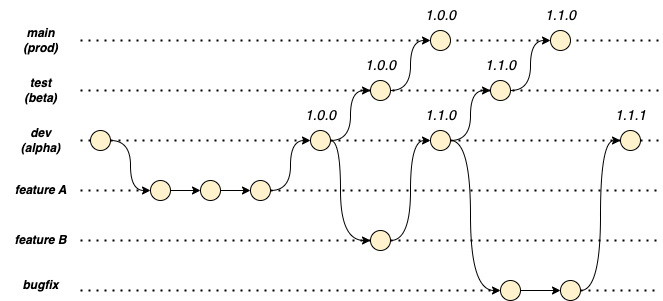
\includegraphics[width=0.65\textwidth]{img/branching-model.png}
        \caption{Esempio di flusso di sviluppo adottando il modello di branching indicato}
        \label{branching}
    \end{figure}
    
    \item \textbf{test} - Branch modificato solamente tramite merge di modifiche provenienti dal branch \textit{dev} con lo scopo di rilasciare una nuova versione \textit{beta} per la validazione esterna.
    \item \textbf{main} - Branch modificato solamente tramite merge di modifiche provenienti dal branch \textit{test} con lo scopo di rilasciare una nuova versione in produzione (\textit{prod}).
\end{itemize}

Grazie ai meccanismi di automazione a supporto della CI/CD fornite dal CI Server si definiscono specifiche regole di attivazione, chiamate \textit{trigger rules}, che permettono di indicare quando uno specifico job deve essere eseguito. Queste regole si basano su eventi che si verificano sul sistema di versionamento come ad esempio commit, tag e merge request. Tramite questa funzionalità è possibile dunque discriminare quali file sono stati modificati e su quale branch per eseguire le operazioni associate come descritto sopra.

\begin{figure}[H]
    \centering
    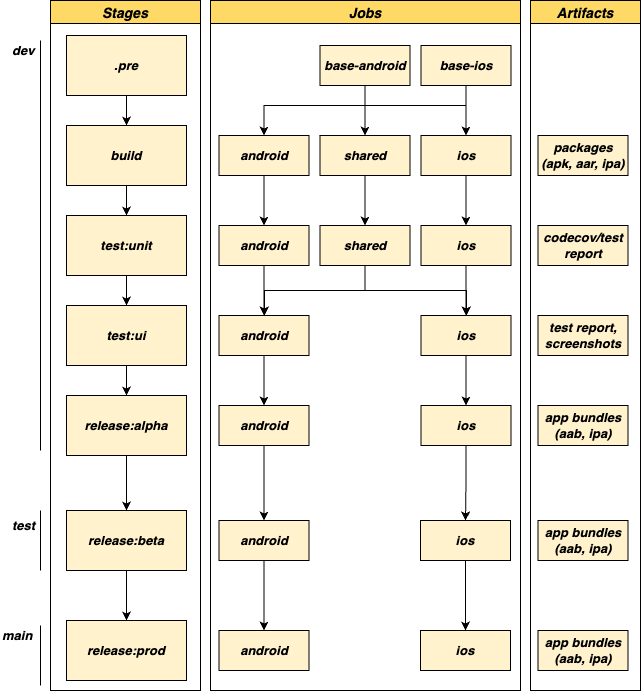
\includegraphics[width=0.85\textwidth]{img/cicd-branch-jobs.png}
    \caption{Stage, job e artefatti associati agli eventi sui branch che compongono l'intera pipeline}
\end{figure}

\section{Templating}
% strumenti utilizzati per favorire il riuso della cicd realizzata

\section{Continuous Integration}
\subsection{Pre}
Molti dei passi che compongono una pipeline utilizzano tipicamente gli stessi tools e le stesse configurazioni per svolgere task diversi. Ad esempio la compilazione del codice e l'esecuzione degli unit test per una applicazione Java utilizzano in entrambi i casi la stessa JDK\footnote{Java Development Kit}, lo stesso tool di build automation e devono essere scaricate le stesse dipendenze di progetto dal package manager di riferimento.

Utilizzando meccanismi di caching e passaggio di artefatti tra i vari job è possibile eseguire tutti quei task di configurazione una sola volta all'inizio della pipeline risparmiando tempo e risorse in tutte le fasi successive.

Nel caso della pipeline progettata per lo sviluppo di applicazioni multipiattaforma con KMM è necessario eseguire i seguenti task di configurazione iniziale:
\begin{itemize}
    \item Configurazione dell'ambiente per lo sviluppo Kotlin tramite l'installazione e il caching degli SDK e del sotto-compilatore \textit{Kotlin/Native}\footnote{\href{https://kotlinlang.org/docs/native-improving-compilation-time.html\#general-recommendations}{https://kotlinlang.org/docs/native-improving-compilation-time.html\#general-recommendations}} per lo sviluppo multipiattaforma.
    \item Configurazione dell'ambiente per lo sviluppo Android tramite l'installazione del SDK Android target e dei vari tools necessari tramite \textit{sdkmanager}\footnote{\href{https://developer.android.com/studio/command-line/sdkmanager}{https://developer.android.com/studio/command-line/sdkmanager}}.
    \item Configurazione dell'ambiente per lo sviluppo iOS tramite impostazione di XCode e CLI Developer Tools.
    \item Installazione e caching di tutte le dipendenze dei vari moduli.
    \item Configurazione delle chiavi per l'autenticazione ai servizi cloud forniti da Google e Apple.
\end{itemize}

Il seguente codice\footnote{\href{https://github.com/paganellif/DevOps-per-applicazioni-mobile-un-caso-di-studio-industriale/blob/5-automazione-del-processo-di-sviluppo/kmm-templates/kmm-base.yml}{https://github.com/paganellif/DevOps-per-applicazioni-mobile-un-caso-di-studio-industriale/blob/5-automazione-del-processo-di-sviluppo/kmm-templates/kmm-base.yml}} mostra il job di pre-configurazione per tutti i job successivi riguardanti la piattaforma Android:

\begin{listing}[H]
    \inputminted{yaml}{code/pre-android-job.yaml}
    \caption{Job di pre-configurazione Android}
\end{listing}

\subsection{Build e Packaging}
Tipicamente la fase di integrazione continua inizia con la verifica della corretta compilazione del codice sorgente. La compilazione rappresenta un vincolo essenziale per tutte le successive fasi e per questo è definita come fase bloccante: in caso di compilazione fallita la pipeline termina senza procedere con le fasi successive definite.

Nel caso dello sviluppo di applicazioni mobile, per lo stage iniziale di build la pratica più diffusa è quella di validare sia la compilazione del codice che la pacchettizzazione della applicazione nei formati richiesti dalle piattaforme target. Dato il funzionamento di una applicazione KMM (Capitolo \ref{ch:app-multiplatform}) è necessario compilare il codice del modulo condiviso \textit{shared} e quello specifico delle piattaforme Android e iOS e impacchettarlo negli artefatti che verranno passati in input alla fase di delivery, rispettivamente aar\footnote{Android Library}, aab e ipa.

Il seguente codice\footnote{\href{https://github.com/paganellif/DevOps-per-applicazioni-mobile-un-caso-di-studio-industriale/blob/5-automazione-del-processo-di-sviluppo/kmm-templates/kmm-build.yml}{https://github.com/paganellif/DevOps-per-applicazioni-mobile-un-caso-di-studio-industriale/blob/5-automazione-del-processo-di-sviluppo/kmm-templates/kmm-build.yml}} mostra il template che definisce il job base di compilazione e pacchettizzazione della applicazione Android tramite l'utilizzo combinato di fastlane e gradle:
\begin{listing}[H]
    \inputminted{yaml}{code/build-job.yaml}
    \caption{Pipeline job dedicato alla compilazione e pacchettizzazione della applicazione Android}
\end{listing}

\subsection{Testing}

\subsection{Dependency Management}

\section{Continuous Delivery}

\subsection{Alpha/Beta Release}

\section{Continuous Inspection}
% progettazione e implementazione analisi


\chapter{Sviluppo applicazione MaggioliEbook}
\label{ch:ch5}
% !TeX root = ../main.tex

\section{Introduzione}

\section{Progettazione}
% progettazione app con mentalità multiplatform

\section{Implementazione modulo condiviso}
% implementazione modulo shared

\section{Implementazione Android}
% implementazione app android

\section{Implementazione iOS}
% implementazione app iOS

\chapter{Risultati raggiunti}
\label{ch:ch6}
% !TeX root = ../main.tex

\section{Introduzione}
In questo capitolo vengono mostrati i risultati ottenuti dalla realizzazione della applicazione multipiattaforma MaggioliEbook adottando il processo di sviluppo descritto nel capitolo \ref{ch:cicd}.

Vengono inizialmente considerati i requisiti definiti nel capitolo \ref{ch:casodistudio} e paragonati con quanto realizzato. Successivamente sono indicate alcune statistiche e metriche, raccolte principalmente tramite la piattaforma GitLab adottata, al fine di creare un primo modello di confronto per i lavori futuri che saranno svolti in azienda sulle tematiche principali di questo caso di studio industriale.

\section{Riuso}
I template che definiscono gli stage e i relativi job del processo di sviluppo progettato sono stati versionati e organizzati in un apposito repository, come descritto in modo dettagliato nel capitolo \ref{ch:cicd}.

Questa soluzione non solo permette il riuso dell'intera pipeline o di solamente una sua parte, ma abilita anche un processo di lavoro collaborativo fra tutti i possibili utilizzatori per la modifica del processo. Ogni sviluppatore all'interno della azienda è infatti in grado di accedere al repository dei template, visionare i file YAML che definiscono la pipeline e aprire merge request per richiedere la modifica o l'aggiunta di funzionalità necessarie al processo di sviluppo automatizzato. A tal proposito è stato scelto un team di sviluppo all'interno dell'azienda che si occupa di applicazioni mobile per svolgere un primo esperimento di integrazione nel proprio processo di sviluppo, già consolidato su tecnologie puramente native e senza alcun sistema di automazione.

\section{Stabilizzazione e rilascio}
La fase di stabilizzazione e rilascio di entrambe le versioni di applicazione sviluppate tramite Kotlin Multiplatform Mobile sono state realizzate rispettando tutti i vincoli definiti nel capitolo \ref{ch:casodistudio}. Durante il processo di sviluppo del caso di studio è stato infatti possibile rilasciare automaticamente applicazioni, sia Android che iOS, sfruttando la pipeline realizzata. In entrambi i casi sono stati definiti gruppi di tester composti sia dalle figure aziendali esperte di dominio che dai Professori relatori di questa tesi:

\begin{figure}[H]
    \centering
    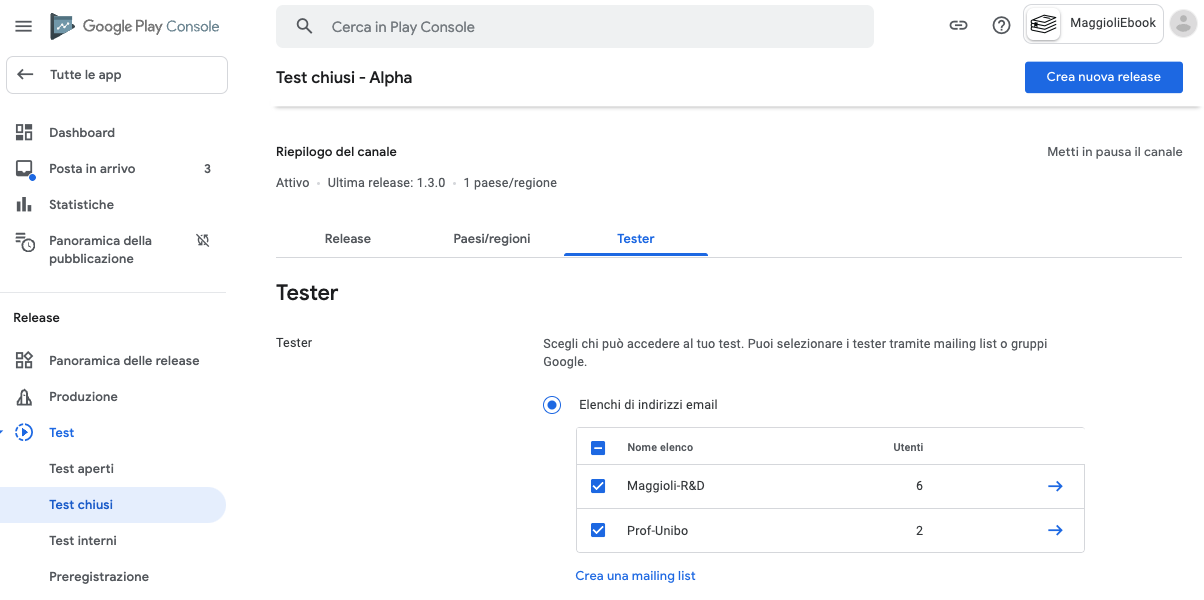
\includegraphics[width=1\textwidth]{img/google-play-console-maggioliebook.png}
    \caption{Schermata Google Play Console per la fase di stabilizzazione della applicazione Android}
    \label{google-play-console-maggioliebook}
\end{figure}

\begin{figure}[H]
    \centering
    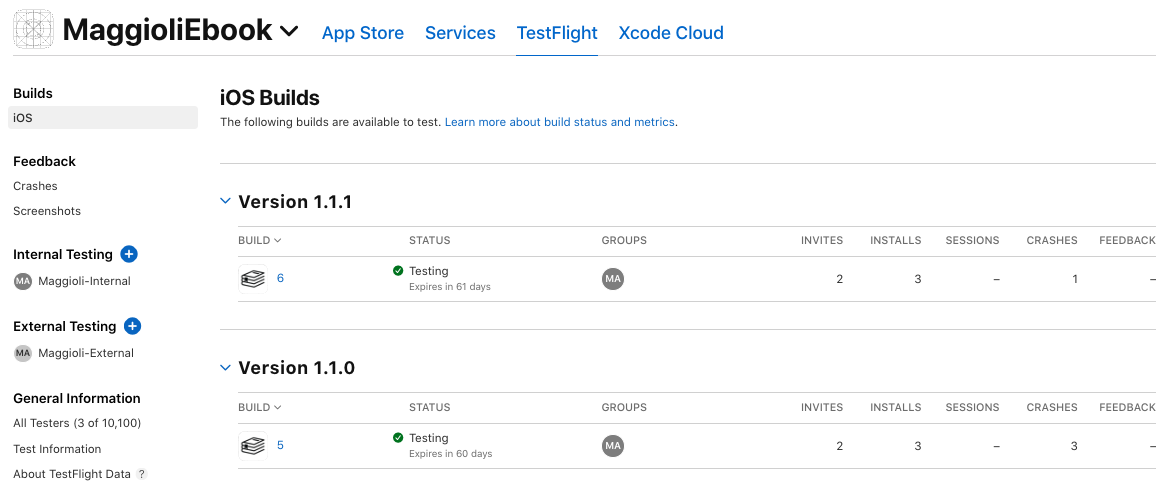
\includegraphics[width=1\textwidth]{img/app-store-connect-maggioliebook.png}
    \caption{Schermata App Store Connect per la fase di stabilizzazione della applicazione iOS}
    \label{app-store-connect-maggioliebook}
\end{figure}

Tutti i tester appartenenti ai gruppi configurati come nelle schermate precedenti sono poi stati in grado di installare con successo l'applicazione sul proprio dispositivo:

\begin{figure}[H]
    \centering
    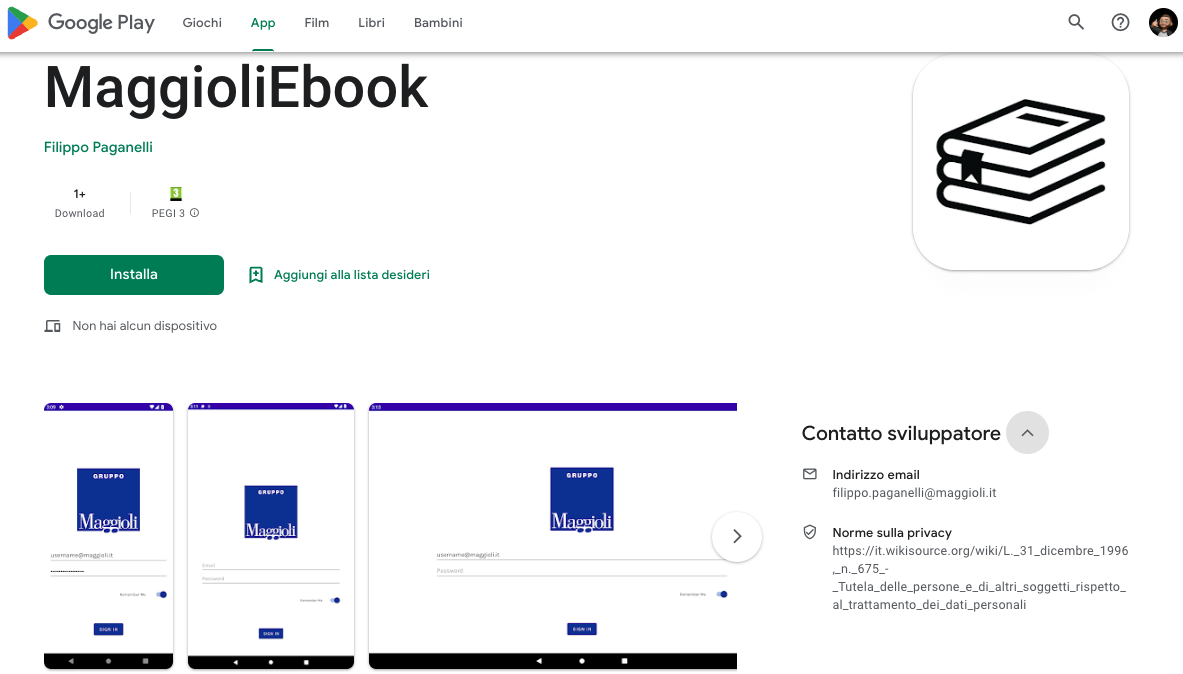
\includegraphics[width=1\textwidth]{img/google-play-store-maggioliebook.png}
    \caption{Schermata Google Play Store per la fase di stabilizzazione della applicazione Android}
    \label{google-play-store-maggioliebook}
\end{figure}

\begin{figure}[H]
    \centering
    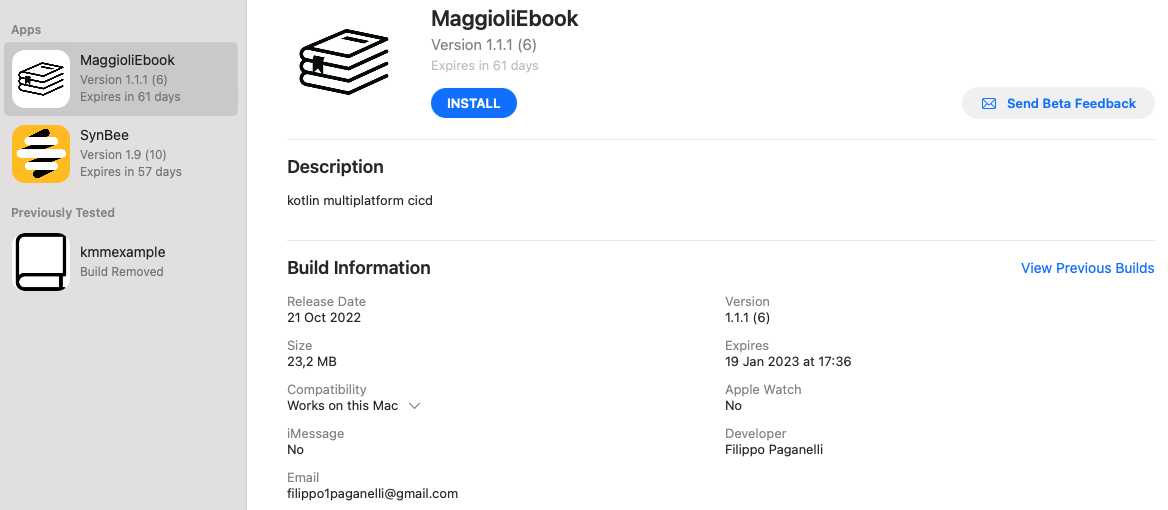
\includegraphics[width=1\textwidth]{img/testflight-maggioliebook.png}
    \caption{Schermata Testflight per la fase di stabilizzazione della applicazione iOS}
    \label{testflight-maggioliebook}
\end{figure}

Un ciclo di stabilizzazione \textit{alpha}-\textit{beta} risulta nell'esecuzione di due pipeline attivate rispettivamente con (\textit{i}) la modifica sul branch \textit{dev} del codice della applicazione e (\textit{ii}) il merge del branch \textit{dev} sul branch \textit{test}. Le seguenti schermate, catturate dalla piattaforma GitLab utilizzata come sistema di versionamento e automazione, mostrano l'esecuzione di un esempio di queste due pipeline nel caso della sola applicazione Android:

\begin{figure}[H]
\centering
    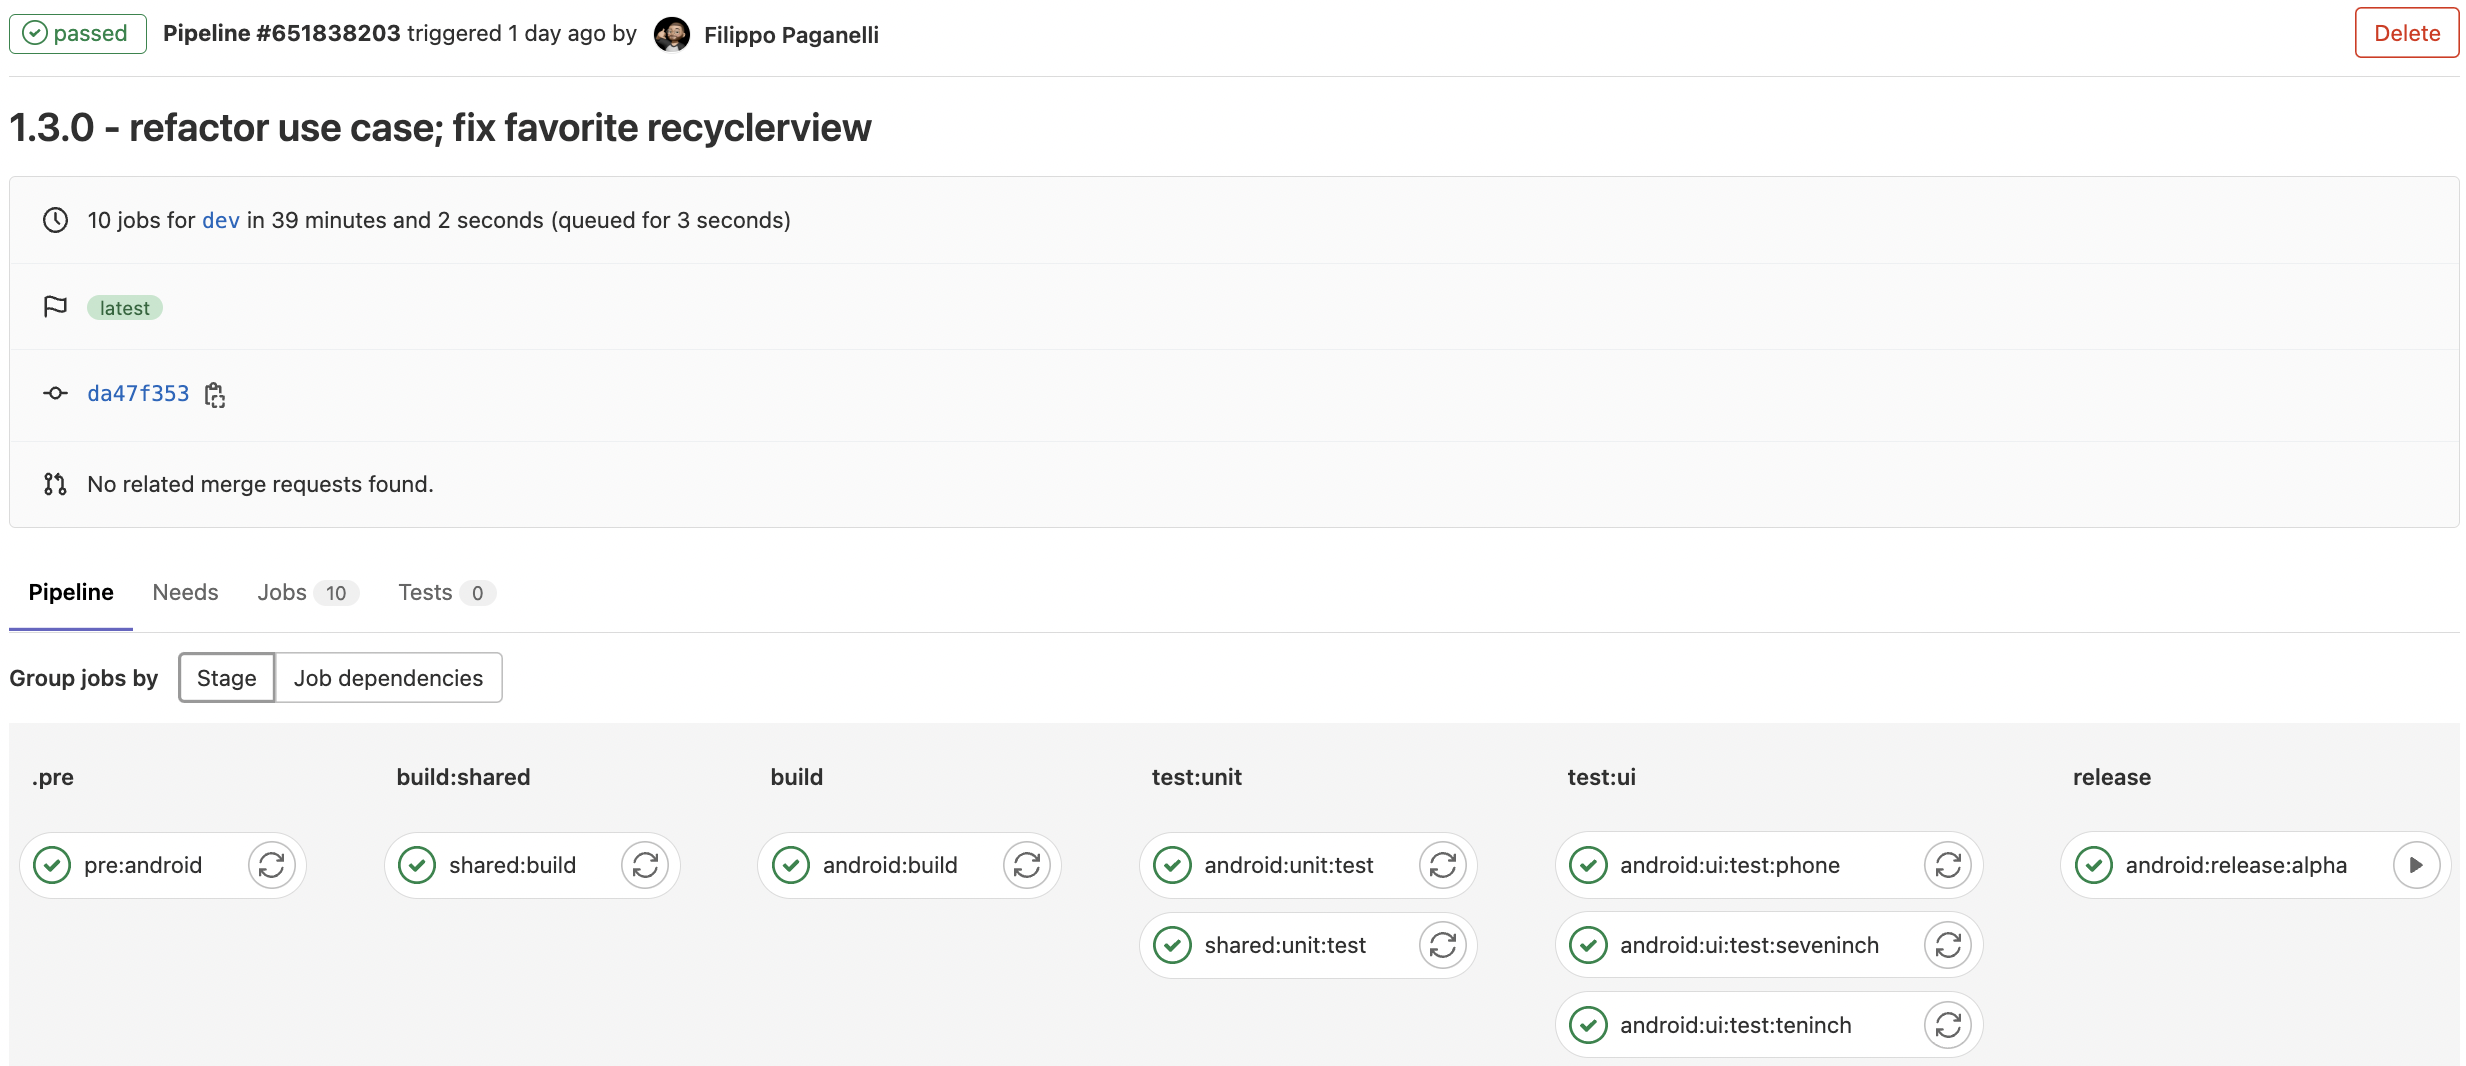
\includegraphics[width=1\textwidth]{img/gitlab-pipeline-android-alpha.png}
    \caption{Schermata GitLab di esecuzione della pipeline completa per il rilascio della applicazione Android in versione \textit{alpha}}
    \label{gitlab-pipeline-android-alpha}
\end{figure}

\begin{figure}[H]
\centering
    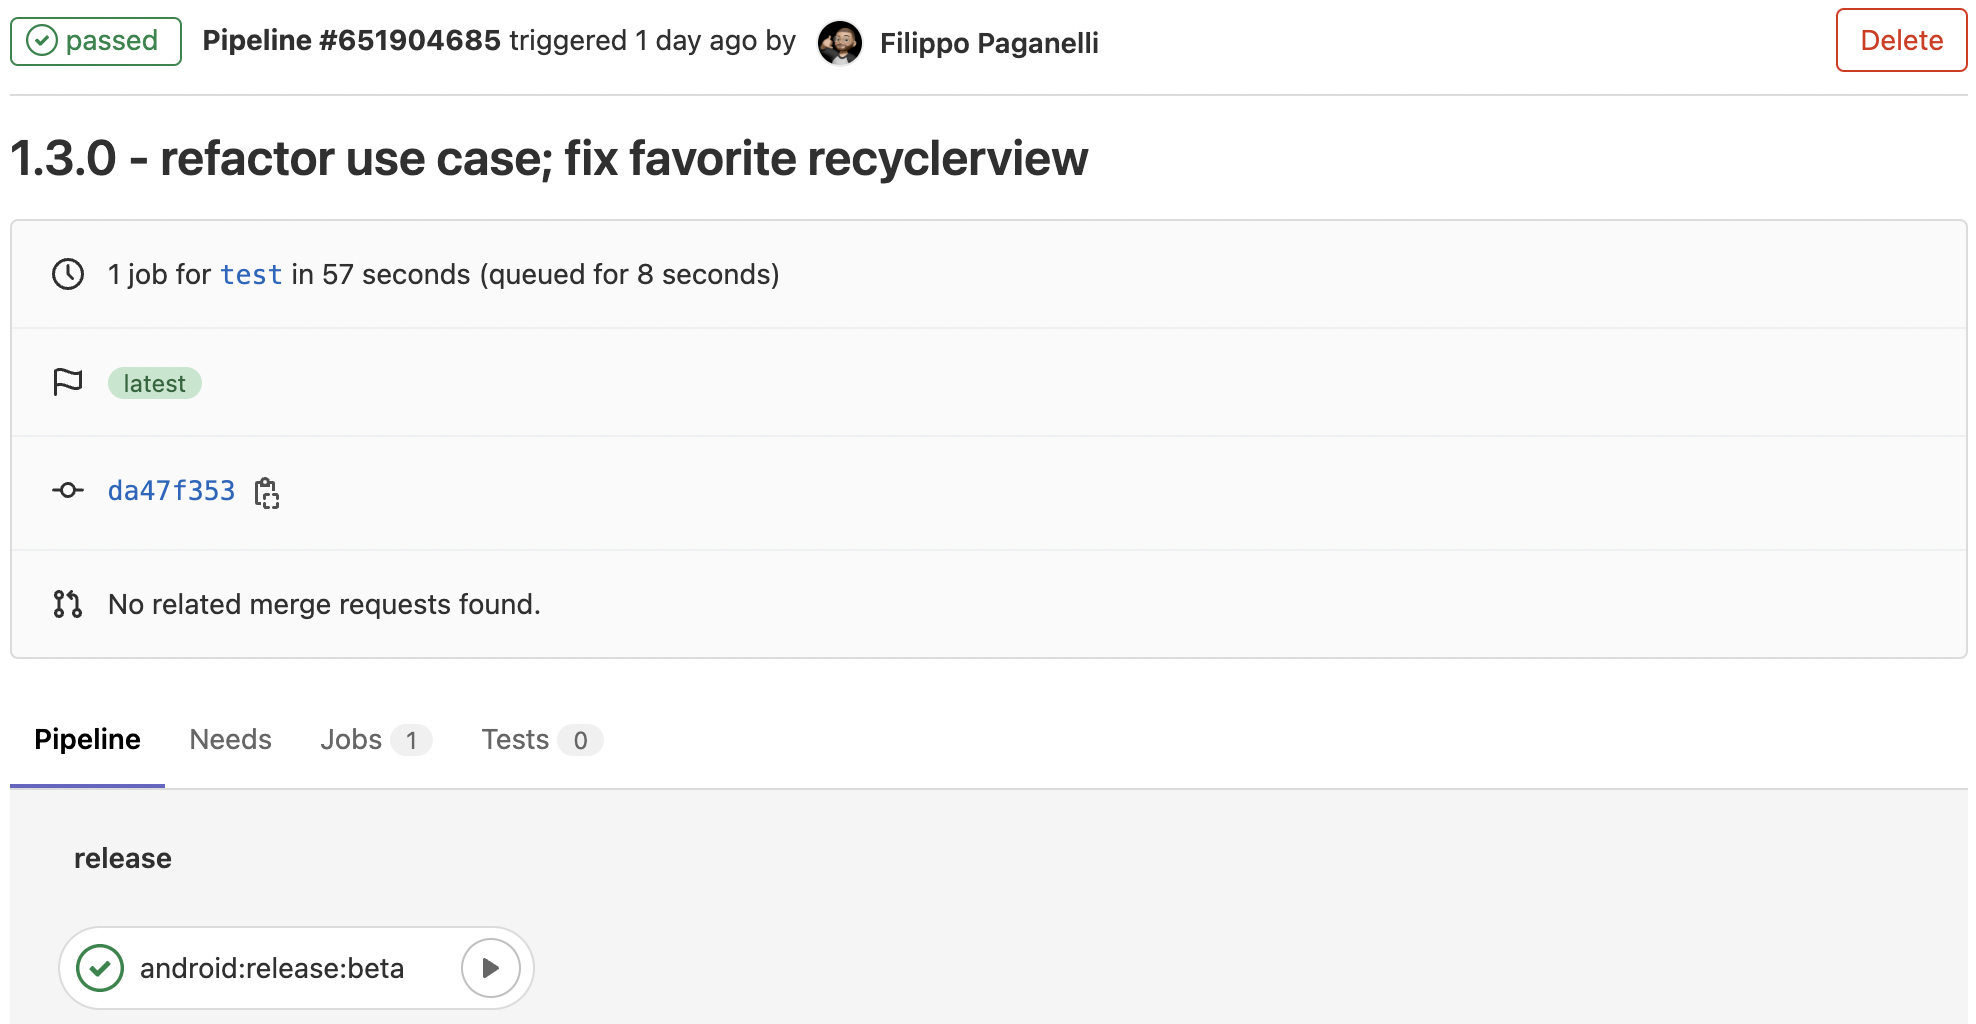
\includegraphics[width=1\textwidth]{img/gitlab-pipeline-android-beta.png}
    \caption{Schermata GitLab di esecuzione della pipeline completa per la promozione da versione \textit{alpha} a versione \textit{beta} della applicazione Android}
    \label{gitlab-pipeline-android-beta}
\end{figure}

\section{Analisi del codice}
% efficacia della pipeline di analisi

\section{Statistiche}
% qualche misurazione delle tempistiche di esecuzione delle pipeline nei vari casi (android, ios, ios+android e rilascio, analisi, ...)
% non ho parametri per fare il confronto rispetto a prima, la app sviluppata è nuova e altri team non hanno cicd app mobile

\section{Lavori futuri}
% cosa ho intenzione di fare dopo, continuazione del lavoro in azienda
\begin{itemize}
        \item Studio, ricerca e sperimentazione per la fase di monitoring, sia della applicazione che dell'utente.
        \item Utilizzo del meccanismo \textit{Remote Configuration}\footnote{\url{https://firebase.google.com/docs/remote-config}} per modificare aspetti della applicazione in modo dinamico senza dover rilasciare nuove versioni. Un esempio tipico è la migrazione dei database: grazie al meccanismo di remote configuration è possibile settare da remoto il \textit{jdbc}\footnote{Java DataBase Connectivity} url che permette di connettersi al database senza dover rilasciare una nuova versione della applicazione con il valore cablato nel codice.
        \item Valutazione di alternative all'hardware Apple fisico. Come indicato nel capitolo \ref{ch:cicd} alcune possibilità individuate sono: (\textit{i}) runner gestiti con sistema operativo MacOS (disponibili su diverse piattaforme come GitLab\footnote{\url{https://docs.gitlab.com/ee/ci/runners/saas/macos_saas_runner.html}}, GitHub\footnote{\url{https://docs.github.com/en/actions/using-github-hosted-runners/about-github-hosted-runners}} e CircleCI\footnote{\url{https://circleci.com/docs/using-macos}}), (\textit{ii}) virtual machine as-a-Service con sistema operativo MacOS (disponibili tra i servizi cloud Amazon\footnote{\url{https://aws.amazon.com/ec2/instance-types/mac/}}) e (\textit{iii}) immagine Docker MacOS\footnote{\url{https://github.com/sickcodes/Docker-OSX}}.
        \item Separazione dei moduli sviluppati in questo caso di studio in modo da avere più repository separati invece che la soluzione monorepo adottata. Distribuzione della logica applicativa sotto forma di libreria kmm e valutazione dei pro e contro di questa soluzione.
        \item Valutazione soluzioni complete as-a-Service. Ad esempio \textit{Bitrise}\footnote{\url{https://www.bitrise.io/}} o XCode Cloud\footnote{\url{https://developer.apple.com/documentation/xcode/xcode-cloud}} (solamente per la parte Apple).
        \item Sperimentazione tecniche CI/CD con tecnologie cross-platform come \textit{Ionic}\footnote{\url{https://ionicframework.com/}}, \textit{Flutter}\footnote{\url{https://flutter.dev/}} o \textit{React Native}\footnote{\url{https://reactnative.dev/}} e stesso caso d'uso (applicazione PoC MaggioliEbook) in modo da avere dei parametri di riferimento e confronto.
\end{itemize}

\chapter{Conclusioni}
\label{ch:ch7}
% !TeX root = ../main.tex

L'output finale di questa tesi dimostra che è stato possibile adottare le pratiche e gli strumenti abilitanti la cultura DevOps per il processo di sviluppo di applicazioni mobile multipiattaforma. Per poter ottenere un sistema di automazione in grado di compilare, testare, impacchettare e rilasciare una applicazione, sia in versione Android che in versione iOS, in circa 28 minuti in media come descritto nei risultati raggiunti (capitolo \ref{ch:risultati}) è stata necessaria una prima fase di analisi approfondita sulla cultura DevOps, sul ciclo di sviluppo delle applicazioni mobile e sui framework multipiattaforma. 

Successivamente è stato individuato un caso di studio per dimostrare l'efficacia della cultura DevOps applicata allo sviluppo mobile multipiattaforma in un contesto industriale. In questa fase sono stati raccolti i requisiti e i vincoli aziendali sia per il processo di sviluppo che per l'applicazione da realizzare in modo da adeguarli a quanto appreso dalla prima fase di studio e definire gli obiettivi reali.




%Per poter misurare con precisione i vantaggi derivanti dalla loro adozione, il sistema è stato realizzato appositamente in modo tale da poter essere integrato velocemente nel processo di sviluppo di altri team in azienda con lo scopo di raccogliere metriche da confrontare con quelle descritte nel capitolo precedente. 

\begin{comment}
\chapter{Mobile Application Development Lifecycle}
\label{ch:ch2}
% !TeX root = ../main.tex

\parindent=0pt
In questo capitolo viene analizzato il processo di sviluppo tipico per le applicazioni mobile al fine di porre le basi per la progettazione dello stesso processo di sviluppo applicando pratiche e tecniche DevOps di automazione. Lo scopo di questa fase iniziale di progetto è quindi la definizione di tutti i principali task e sotto-task necessari allo sviluppo di applicazioni mobile, dalla scrittura del codice sorgente al rilascio sui marketplace delle relative piattaforme target, le quali sono Android e iOS.

\begin{figure}[H]
\centering
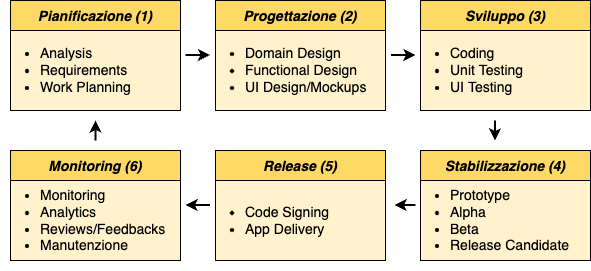
\includegraphics[width=0.75\textwidth]{img/tesi-2-Page-9.drawio.png}
\caption{Ciclo di vita di sviluppo tipico delle applicazioni mobile}
\end{figure}

Il processo di sviluppo delle applicazioni mobile è simile a quello di qualsiasi altra tipologia di applicazione: in questo caso l'obiettivo è distribuire l'applicazione, dando la possibilità all'utente di installarla sul proprio dispositivo, mentre tipicamente nei processi di altre tipologie di applicazioni l'obiettivo è quello di mettere in esecuzione l'applicazione in un ambiente target accessibile all'utente.

\section{Pianificazione}
In questa prima fase del processo di sviluppo si formalizzano i requisiti, funzionali e non funzionali, che devono essere soddisfatti dalla applicazione per ottenere l'approvazione del committente e si pianifica il lavoro per le successive fasi in termini di task, risorse e tempo.\\
Tramite la definizione di casi d'uso si rappresentano le interazioni tra il sistema e dei ruoli (attori in UML\footnote{Unified Modeling Language}) necessarie al raggiungimento di un obiettivo. Questi casi d'uso sono dunque dei possibili scenari dove il sistema riceve delle richieste esterne, come l'input dell'utente, e risponde ad esso.
Dopo aver acquisito un numero appropriato di casi d'uso e attori è molto più semplice iniziare a progettare una applicazione. Lo sviluppo può quindi concentrarsi su come creare l'applicazione anziché sulla sua definizione o la sua funzione.

\section{Progettazione}
La fase di progettazione della applicazione è composta da un insieme di sottotask tra cui la modellazione del dominio applicativo, la scelta della architettura da utilizzare e la prototipazione dell'esperienza utente e dell'interfaccia grafica (UX/UI).\\
Tipicamente la progettazione UX/UI viene svolta tramite l'ausilio di mockup per definire prima come l'utente intende utilizzare l'applicazione (esperienza) e poi aspetti grafici come colori, font e icone (interfaccia).

\section{Sviluppo}
Una volta progettata l'applicazione è possibile partire con la fase di sviluppo. Solitamente l'obiettivo è far iniziare la fase di sviluppo il prima possibile in modo da sviluppare un prototipo funzionante ed ottenere la validazione da parte del committente, la quale è l'obiettivo principale della fase successiva.

\section{Stabilizzazione}
La stabilizzazione consiste nella risoluzione di problemi sia a livello funzionale che a livello di usabilità e di prestazioni al fine di ottenere una versione di applicazione pronta da distribuire. Questa parte del ciclo di sviluppo dovrebbe iniziare il più presto possibile in modo da individuare e risolvere i problemi prima che diventino un costo. Tipicamente per qualsiasi applicazione, anche non specifica per i dispositivi mobile, sono previste le seguenti sottofasi del processo di stabilizzazione\cite{sdlf}:
\begin{itemize}
    \item \textit{Prototype} - L'applicazione include soltanto alcune delle funzionalità principali e sono presenti bug maggiori. In questa fase il focus è sulla singola funzionalità implementata fornita dal prototipo per il testing.
    \item \textit{Alpha} - Tutte le principali funzionalità sono completate e devono essere testate.
    \item \textit{Beta} - Gran parte delle funzionalità, sia principali che ausiliarie, sono state completate e i bug maggiori sono stati risolti.
    \item \textit{Release Candidate} - Tutte le funzionalità sono state completate e testate, ma potrebbero essere presenti ancora bug minori.
\end{itemize}

\subsection{Alpha}
La prima versione funzionante di una applicazione è detta alpha ed è utilizzata per il testing interno di specifiche funzionalità. Questo significa che può presentare anche bug o funzionalità mancanti ma almeno deve contenere le funzionalità che devono essere testate per quella specifica versione alpha. \\
Solitamente prima della release di una applicazione, anche se in fase di testing, è necessario attendere la sua approvazione da parte del gestore del servizio. Il processo di approvazione pre-release è detto \textit{App Review}. Nel caso del testing interno è possibile distribuire la applicazione ad un insieme ristretto di tester.\\
Continuando con i rilasci di versioni alpha vengono aggiunte nuove funzionalità e/o risolti eventuali bug: quando la versione è considerata pronta viene eseguita una sua promozione. Con promozione si intende in questo caso il rilascio di una versione alpha in versione beta.

\subsection{Beta}
A questo punto del processo di sviluppo la applicazione è considerata completa a tutti gli effetti a meno di bug e/o problemi di stabilità. La versione beta rappresenta dunque la prima versione della applicazione resa disponibile ai tester esterni, ovvero quegli utenti che non hanno partecipato alle fasi di sviluppo e che svolgono il ruolo di validazione delle funzionalità. Si distinguono due tipologie di beta testing:
\begin{itemize}
    \item \textit{Aperto} - La applicazione è rilasciata per la fase di testing esterno permettendo l'accesso a qualsiasi utente con account da beta tester. Nel caso di Android per poter testare una applicazione in versione beta aperta è necessario disporre di un account Google Developer.
    \item \textit{Chiuso} - L'accesso alla applicazione di test è limitato ad un insieme ristretto di tester, tipicamente gestiti tramite mailing list o link di condivisione.
\end{itemize}
Dopo aver ottenuto la validazione da parte dei tester, la quale potrebbe richiedere più iterazioni di sviluppo e rilascio di versioni alpha-beta, anche per la versione beta si effettua la promozione, rilasciando la applicazione in produzione.


\section{Release}
Dopo che la applicazione è stata stabilizzata è possibile procedere con la distribuzione. In questa fase l'applicazione viene prima firmata digitalmente utilizzando un certificato protetto da chiave privata e poi pubblicata sullo specifico marketplace della piattaforma target.


\section{Monitoraggio}
La fase di monitoraggio (e manutenzione) è quella più lunga e dispendiosa in termini di tempo e risorse. Per le applicazioni mobile esistono alcune situazioni che rendono il monitoraggio più complesso rispetto ad altre tipologie di applicazioni come ad esempio le web app. Bisogna infatti considerare che\cite{mamonitoring}:
\begin{itemize}
    \item le applicazioni mobile eseguono su una vasta gamma di dispositivi con caratteristiche diverse e può essere quindi difficile ottenere una chiara visibilità delle prestazioni lato client;
    \item se gli utenti riscontrano un problema, mentre una patch per applicazioni web può essere distribuita quasi all'istante, la distribuzione degli aggiornamenti delle applicazioni mobile richiede tempo e l'attivazione da parte degli utenti per scaricarli.
\end{itemize}
Per effettuare un monitoraggio efficace è necessario misurare e controllare continuamente le performance della applicazione mobile, il comportamento dell'utente e gli errori che essi riscontrano. Alcuni esempi di metriche fondamentali sono: tempo di avvio della applicazione, network performance, utilizzo delle risorse (CPU, disco e memoria) e metriche custom derivanti dalle azioni dell'utente.

\chapter{Tools}
\label{ch:ch3}
% !TeX root = ../main.tex

\section{Kotlin Multiplatform Mobile}
\parindent=0pt
Kotlin Multiplatform Mobile\footnote{\url{https://kotlinlang.org/lp/mobile/}} (KMM) è un framework per lo sviluppo di app iOS e Android basato sul concetto di condivisione della logica applicativa mantenendo lo sviluppo nativo della UX/UI\footnote{User Experience/User Interface}. Consiste in un caso d'uso specifico (e il più diffuso) del framework Kotlin MultiPlatform (KMP), il quale permette di sviluppare il codice in modo agnostico rispetto le piattaforme target e di condividerlo tra differenti piattaforme facendo uso dei tre principali compilatori inclusi nell'ecosistema Kotlin\cite{nagy2022simplifying}:
\begin{itemize}
    \item Kotlin/JVM (Android, Spring, ...)
    \item Kotlin/Native (iOS, macOS, ...)
    \item Kotlin/JS (Web)
\end{itemize}
KMM dipende fortemente dai compilatori Kotlin/JVM (Android) e Kotlin/Native (iOS) e fornisce benefici derivanti sia dallo sviluppo cross-platform che dallo sviluppo nativo:
\begin{itemize}
    \item risparmio di tempo e risorse derivanti dalla condivisione del codice (cross-platform),
    \item alte performance (nativo),
    \item accesso diretto alle funzionalità dei dispositivi hardware senza overhead (nativo).
\end{itemize}

\begin{figure}[H]
\centering
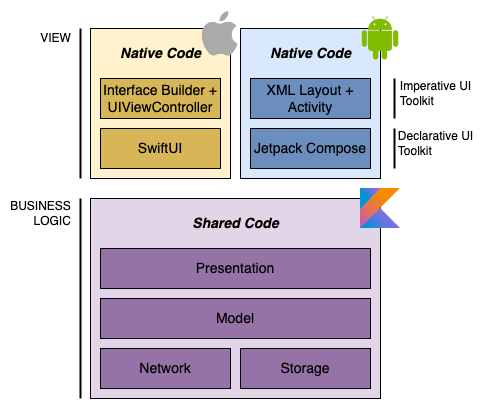
\includegraphics[width=0.7\textwidth]{img/tesi-8-kmm.drawio.png}
\caption{Architettura Kotlin Multiplatform Mobile}
\end{figure}

Con il rilascio di Kotlin 1.4 (Agosto 2020), KMM è passato dalla fase "\textit{Experimental}" alla fase "\textit{Alpha}" la quale è considerata come fase "\textit{pre-stable}"\footnote{\url{https://kotlinlang.org/docs/components-stability.html\#stability-levels-explained}} ma è comunque già stato adottato in produzione per lo sviluppo delle proprie applicazioni mobile da tantissime aziende tra le quali è possibile trovare nomi rilevanti come Netflix, VMware e Philips\footnote{\url{https://kotlinlang.org/lp/mobile/case-studies/}}.\\
In base al risultato dell'indagine di mercato svolta nei primi due quadrimestri del 2021\cite{kmm2}, le porzioni di codice condiviso nelle applicazioni sviluppate con KMM sono:
\begin{itemize}
    \item 85\% Networking
    \item 75\% Data Storage
    \item 70\% Utility (Logging, Analytics, ...)
    \item $\sim$60\% Algoritmi/Computazione
    \item $\sim$55\% State Management
    \item $\sim$50\% Presenters/Controllers/ViewModel
\end{itemize}

\subsection{Kotlin/JVM}
Il compilatore Kotlin/JVM è uno dei due compilatori su cui è basato KMM, utilizzato per la piattaforma Android. Permette di compilare codice Kotlin in bytecode Java (\textit{.class}), il quale può essere eseguito direttamente sulla JVM. Nel caso di Android è necessario un ulteriore passaggio per tradurre il bytecode Java in bytecode Dalvik (\textit{.dex}).

\begin{figure}[H]
\centering
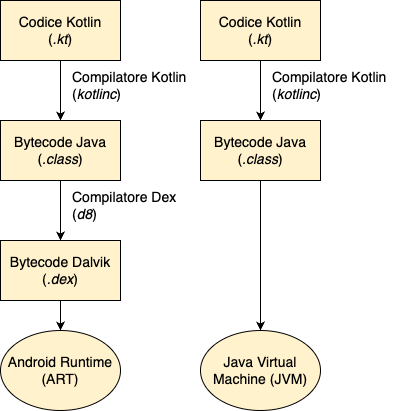
\includegraphics[width=0.55\textwidth]{img/tesi-9-kotlinjvm.drawio.png}
\caption{Fasi di compilazione Kotlin/JVM con piattaforma target Android e JVM}
\end{figure}

\subsection{Kotlin/Native}
Kotlin/Native è il secondo compilatore su cui è basato KMM e viene utilizzato per la piattaforma iOS. A differenza del compilatore Kotlin/JVM, il compilatore Kotlin/Native è progettato per quelle situazioni dove non è possibile o non si vuole avere una VM come nel caso dei dispositivi embedded e della piattaforma iOS. Per fare ciò include un backend basato su \textit{Low Level Virtual Machine} (LLVM)\footnote{\url{https://llvm.org/}}, ovvero il codice Kotlin viene compilato in binari nativi che possono essere eseguiti senza VM\cite{nagy2022simplifying}. Le piattaforme supportate da Kotlin/Native attualmente sono macOS, iOS, tvOS, watchOS, Linux, Windows (MinGW) e Android NDK\footnote{\url{https://kotlinlang.org/docs/native-overview.html\#target-platforms}} e per ognuna di esse esistono differenti architetture. Nel caso di iOS le differenti architetture supportate da KMM sono \textit{Arm64}, \textit{Arm32} e \textit{x64}.
\begin{figure}[H]
\centering
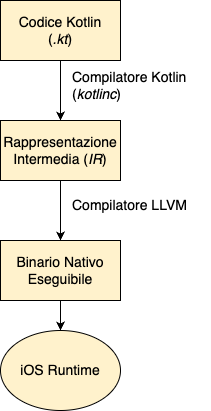
\includegraphics[width=0.28\textwidth]{img/tesi-10-kotlinnative.drawio.png}
\caption{Fasi di compilazione Kotlin/Native con piattaforma target iOS}
\end{figure}
Anche in questo caso sono necessarie due fasi di compilazione: ($i$) il codice Kotlin viene compilato nella \textit{Rappresentazione Intermedia} (IR) LLVM e ($ii$) successivamente compilato nel binario nativo.

\subsection{Expect/Actual}
Quando si sviluppa codice condiviso è spesso necessario definire come determinate funzionalità debbano essere implementate sulla specifica piattaforma target per utilizzare i relativi SDK. Il framework KMP fornisce il meccanismo \textit{expect/actual} per assolvere a questo compito in modo analogo al design pattern \textit{Template Method}:
\begin{itemize}
    \item \textit{Expect} - Astrazione della funzionalità necessaria. Tramite la keywork \textit{expect} si definisce lo scheletro astraendo dalla specifica implementazione.
    \item \textit{Actual} - Implementazione specifica per una determinata piattaforma. Tramite la keywork \textit{actual} si definisce l'implementazione, reificando l'altrazione definita tramite il concetto di \textit{expect}.
\end{itemize}

\begin{listing}[H]
\inputminted{kotlin}{code/3-expectactual}
\caption{Esempio di applicazione expect/actual per ottenere informazioni sulla piattaforma}
\end{listing}

\subsection{Plugin Gradle KMP}
Il plugin Gradle KMP è uno strumento utile per realizzare progetti multiplatform. Fornisce uno specifico DSL\footnote{Domain Specific Language} per definire e configurare i task necessari a compilare il codice condiviso per le relative piattaforme target\footnote{\url{https://kotlinlang.org/docs/multiplatform-dsl-reference.html}}. Al momento la versione latest (stable) del plugin è la \textit{1.6.21}, rilasciata il 19/04/2022\footnote{\url{https://plugins.gradle.org/plugin/org.jetbrains.kotlin.multiplatform/1.6.21}} ma è presente una versione candidata per il rilascio con tag \textit{1.7.0-RC2}.

\begin{listing}[H]
\inputminted{kotlin}{code/3-gradlekmm1}
\caption{Struttura iniziale del file \textit{settings.gradle.kts} nella root di progetto (Kotlin)}
\end{listing}

\begin{listing}[H]
\inputminted{kotlin}{code/3-gradlekmm2}
\caption{Definizione utilizzo Plugin Gradle KMP nel file \textit{build.gradle.kts} del modulo condiviso (Kotlin)}
\end{listing}

\subsubsection{Plugin Tasks}
Il plugin gradle KMM e le relative dipendenze rendono disponibile una vasta serie di task per eseguire differenti elaborazioni sia sul codice della specifica piattaforma target che sul codice condiviso. Alcune delle principali tipologie di task sono:
\begin{itemize}
    \item Build - tasks per build, compile, link
    \item CocoaPods - tasks per la gestione delle dipendenze Swift/Objective-C
    \item Interop - tasks relativi all'utilizzo del \textit{commonizer}\footnote{\url{https://github.com/JetBrains/kotlin/tree/master/native/commonizer}}
    \item Verification tasks - tasks per l'esecuzione dei test
\end{itemize}

\subsubsection{KMM Android Studio IDE Plugin}
L'IDE\footnote{Integrated Development Environment} Android Studio è costruito su IntelliJ, il quale è uno tra gli IDE più diffusi ed è sviluppato da JetBrains. Tramite il plugin KMM, installabile direttamente dal marketplace integrato in Android Studio o dal sito ufficiale JetBrains\footnote{\url{https://plugins.jetbrains.com/plugin/14936-kotlin-multiplatform-mobile/versions/stable}}, si abilita un insieme di funzionalità a supporto dello sviluppo di codice multiplatform, in particolare:
\begin{itemize}
    \item creazione della struttura e della configurazione base per una nuova applicazione multiplatform,
    \item creazione della struttura e della configurazione base per una nuova libreria multiplatform,
    \item integrazione di moduli multiplatform in applicazioni già esistenti.
\end{itemize}

\section{Fastlane}
Uno fra i tool open source più diffusi a supporto della automazione dello sviluppo di applicazioni mobile, sia Android che iOS, è Fastlane\footnote{\url{https://github.com/fastlane/fastlane}}. L'impiego principale di questo tool sviluppato in Ruby consiste nella automazione della fase di rilascio della applicazione, sia in beta che in produzione, grazie alla gestione di tutti quei task necessari ma dispendiosi in termini di tempo come ad esempio la generazione degli screenshot e la firma digitale del codice (\textit{Code Signing}).\\
Si fa uso dei seguenti concetti per controllare il comportamento di fastlane negli appositi file di configurazione \textit{Fastfile} e \textit{Appfile}:
\begin{itemize}
    \item \textit{Action} - Elaborazioni pre-definite e configurabili tramite passaggio di parametri.
    \item \textit{Lane} - Insieme di action definito dall'utente per descrivere elaborazioni complesse.
\end{itemize}

\begin{listing}[H]
\inputminted{ruby}{code/4-fastlane}
\caption{Esempio di definizione di un lane per il rilascio in versione beta di applicazioni iOS}
\end{listing}

I file \textit{Fastfile} e \textit{Appfile}, i quali risiedono nella cartella \textit{fastlane} nella root di progetto, sono utilizzati rispettivamente per definire configurazioni globali a livello di applicazione e per definire il comportamento di fastlane. Per questo motivo è necessario configurare fastlane per ogni modulo che si intende utilizzare, sia che esso sia una libreria o una applicazione. Nel caso di applicazioni multiplatform è quindi necessario per tutti i tre moduli \textit{shared}, \textit{androidApp} e \textit{iosApp}.\\
Nelle successive descrizioni delle fasi che compongono la pipeline progettata viene indicato come è stato configurato e adottato Fastlane ove utilizzato. 

\chapter{CI/CD}
\label{ch:ch4}
% !TeX root = ../main.tex

Dato il processo di sviluppo delle applicazioni mobile individuato nel capitolo \ref{ch:ch3} e definiti gli strumenti e task necessari, si descrive in questo capitolo come è stato automatizzato il processo adottando le moderne tecniche di integrazione continua e rilascio continuo al fine di fornire un modello di processo di sviluppo ai vari reparti aziendali che si occupano di applicazioni mobile.

\section{Continuous Integration}

\section{Continuous Delivery}

\section{Continuous Monitoring}

\section{Infrastruttura}
% descrivere l'infrastruttura necessaria a supporto della cicd runners, nexus, defectdojo, ....

\section{Templating}
% definire la cicd in template in un progetto a parte in modo che possano essere importati nel PoC (ed essere usati da altri in futuro)
% dire come gitlab permette di farlo, quali sono i meccanismi ecc ecc
% lo stesso risultato può essere ottenuto distribuendo delle github action



\chapter{Caso d'uso: App PoC MaggioliEbook}
\label{ch:ch5}
% !TeX root = ../main.tex
In questo capitolo viene descritto un caso d'uso aziendale di sviluppo di applicazione mobile adottando i metodi, gli automatismi e gli strumenti descritti nel capitolo \ref{ch:ch4}. L'obiettivo è quello di dimostrare l'efficacia del modello progettato tramite lo sviluppo di una applicazione mobile per la gestione e la visualizzazione dei contenuti digitali pubblicati da Maggioli SpA in formato ebook e rilasciata per le piattaforme Android e iOS.

\section{Analisi dei Requisiti}
\subsection{Requisiti Funzionali}
\begin{itemize}
    \item \textbf{R1} - Visualizzazione documenti.
    \begin{itemize}
        \item \textbf{R1.1} - In modo fluido, mostrando il contenuto adattato al dispositivo in cui viene mostrato.
        \item \textbf{R1.2} - In modo statico, mostrando il contenuto con uno specifico layout indipendente dal dispositivo in cui viene mostrato.
    \end{itemize}
    \item \textbf{R2} - Modifica documenti fluidi (lato utente).
    \begin{itemize}
        \item \textbf{R2.1} - Aggiunta commenti, sottolineature, evidenziazioni, al contenuto fluido.
        \item \textbf{R2.2} - Memorizzazione commenti, sottolineature, evidenziazioni apportate al contenuto fluido.
    \end{itemize}
    \item \textbf{R3} - Gestione utente.
    \begin{itemize}
        \item \textbf{R3.1} - Login (autenticazione) utente.
        \item \textbf{R3.2} - Visualizzazione documenti a cui l'utente è abbonato.
    \end{itemize}
    \item \textbf{R4} - Ricerca documenti.
    \item \textbf{R5} - Conversione documenti da modo statico a modo fluido.
    \item \textbf{R6} - Modifica documenti in modo fluido (lato azienda).
    \begin{itemize}
        \item \textbf{R6.1} - Aggiunta elementi/contenuti al documento in modo fluido (hyperlink, quiz, video, immagini, ...).
        \item \textbf{R6.2} - Memorizzazione elementi/contenuti aggiunti al documento fluido (hyperlink, quiz, video, immagini, ...).
    \end{itemize}
\end{itemize}

\begin{figure}[H]
\centering
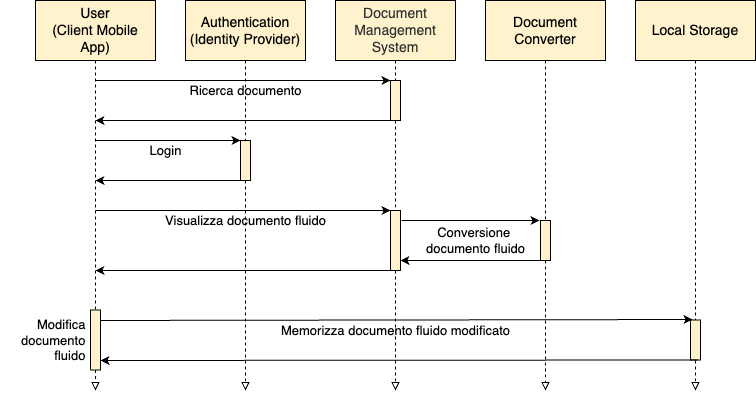
\includegraphics[width=1\textwidth]{img/tesi-2-Use-case2.drawio.png}
\caption{UML - Diagramma di sequenza: scenario di modifica di un nuovo documento "fluido"}
\end{figure}

\subsection{Requisiti Non Funzionali/Tecnologici}
\begin{itemize}
    \item \textbf{T1} - Applicazione nativa Android e iOS, sfruttando Kotlin Multiplatform Mobile (KMM).
    \item \textbf{T2} - Continuous Integration e Continuous Delivery
    \begin{itemize}
        \item \textbf{T2.1} - Analisi statica del codice (SAST\footnote{Static Application Security Testing}).
        \item \textbf{T2.2} - Unit testing, code coverage e E2E\footnote{End-to-End} testing.
        \item \textbf{T2.3} - Rilascio automatico nei relativi store delle piattaforme scelte (Google Play per Android e App Store per iOS).
    \end{itemize}
\end{itemize}

\subsection{Ubiquitous Language}
Per far si che la successiva fase di modellazione del dominio sia efficace è necessario che il team di sviluppo, composto da figure tecniche, e i committenti, i quali sono invece esperti di dominio, utilizzino lo stesso linguaggio. Il concetto di \textit{Ubiquitous Language} definisce un vocabolario condiviso da entrambe le parti per la discussione del software\cite{evans_domain-driven_2004}.\\
Il seguente glossario racchiude tutti i principali termini utilizzati negli incontri tra team di sviluppo ed esperti di dominio:

\begin{table}[H]
\centering
    \begin{tabular}{|c|c|}
         \hline
         \textbf{Termine} & \textbf{Descrizione}\\
         \hline
         \textit{Reader} & \specialcell{Lettore di documenti in grado di visualizzarlo ed \\interagire con esso.}\\
         \hline
         \textit{Documento} & Contenuto digitale pubblicato da Maggioli Editore.\\
         \hline
         \textit{Documento Statico} & Documento con una certa struttura definita nel formato (PDF).\\
         \hline
         \textit{Documento Fluido} & \specialcell{Documento senza struttura in grado di adattarsi al dispositivo\\ in cui viene aperto (EPUB).}\\
         \hline
         \textit{Libro} & \specialcell{Tipologia principale di documento fluido fruibile\\ tramite l'applicazione MaggioliEbook.}\\
         \hline
         \textit{Rivista} & \specialcell{Tipologia principale di documento statico fruibile\\ tramite l'applicazione MaggioliEbook.}\\
         \hline
         \textit{Bookmark} & Identifica una specifica pagina di un libro o di una rivista.\\
         \hline
         \textit{Progression} & \specialcell{Progresso di lettura di un libro o di una rivista,\\ calcolato in percentuale (totale di pagine lette sul totale di pagine\\ del documento).}\\
         \hline
         \textit{Highlight} & \specialcell{Annotazione per una certa porzione testuale di \\documento. Può essere una evidenziazione, sottolineatura \\o annotazione testuale.}\\
         \hline
         \textit{Favorite} &  Documento preferito dall'utente.\\
         \hline
         \textit{User} & Utente con uno o più abbonamenti attivi.\\
         \hline
          \textit{Token} & \specialcell{Autentica e autorizza l'utente ad accedere ai vari documenti\\ per i quali esiste un abbonamento attivo.}\\
         \hline
    \end{tabular}
    \caption{Glossario dei termini (MaggioliEbook Ubiquitous Language)}
\end{table}

I seguenti glossari definiscono invece alcuni dei principali eventi del sistema, suddivisi tra \textit{Incoming Events} e \textit{Outcoming Events}:

\begin{table}[H]
\centering
    \begin{tabular}{|c|c|}
         \hline
         \textbf{Incoming Events} & \textbf{Descrizione}\\
         \hline
         \textit{Apertura documento} & Richiesta di apertura in lettura di uno specifico documento.\\
         \hline
         \textit{Chiusura documento} & Richiesta di chiusura del documento aperto in lettura.\\
         \hline
         \textit{Ricerca documento} & Richiesta di ricerca documento tramite query testuale.\\
         \hline
         \textit{CRUD Highlight} & \specialcell{Richiesta di creazione, lettura, aggiornamento o \\eliminazione di annotazioni.}\\
         \hline
         \textit{CRUD Bookmark} & \specialcell{Richiesta di creazione, lettura, aggiornamento o \\eliminazione di segnalibri.}\\
         \hline
          \textit{CRUD Favorite} & \specialcell{Richiesta di creazione, lettura, aggiornamento o \\eliminazione dei preferiti.}\\
         \hline
    \end{tabular}
    \caption{Glossario degli eventi in ingresso (MaggioliEbook Incoming Events)}
\end{table}

\begin{table}[H]
\centering
    \begin{tabular}{|c|c|}
         \hline
         \textbf{Outcoming Events} & \textbf{Descrizione}\\
         \hline
         \specialcell{\textit{Conversione}\\\textit{PDF2EPUB}} & \specialcell{Richiesta di conversione di un documento statico in\\ documento fluido (dal formato PDF al formato EPUB).}\\
         \hline
         \textit{Ricerca documento} & Richiesta di ricerca documento tramite query testuale.\\
         \hline
         \specialcell{\textit{Download contenuto}\\\textit{documenti}} & Scaricamento del contenuto dei documenti.\\
         \hline
         \specialcell{\textit{Download copertina}\\\textit{documenti}} & Scaricamento della immagine di copertina dei documenti.\\
         \hline
         \specialcell{\textit{Autenticazione}\\\textit{user}} & Richiesta di autenticazione dell'utente (ottenimento token).\\
         \hline
    \end{tabular}
    \caption{Glossario degli eventi in uscita (MaggioliEbook Outcoming Events)}
\end{table}

\begin{figure}[H]
\centering
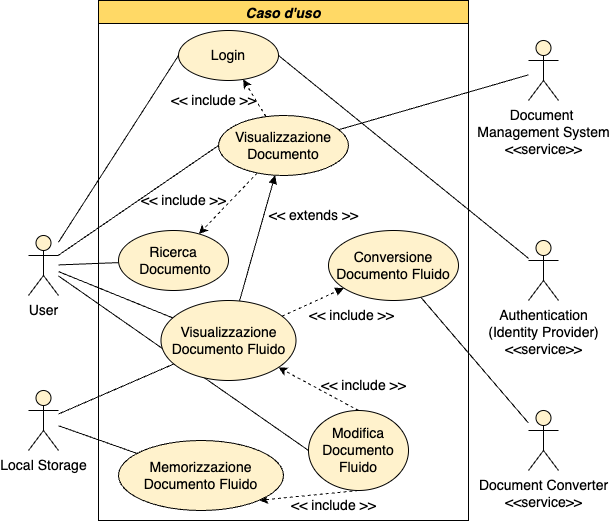
\includegraphics[width=1\textwidth]{img/tesi-1-Use-case.drawio.png}
\caption{UML - Diagramma dei casi d'uso: funzioni/servizi offerti dal sistema Ebook App PoC}
\end{figure}

\section{Analisi Formati Digitali Fluidi}
I documenti attualmente sono reperibili in formato PDF e/o HTML. Il formato PDF è quello con cui i documenti vengono effettivamente archiviati: per ottenere un documento in formato HTML è necessario utilizzare un servizio interno, chiamato \textit{pdf2html}, il quale effettua la conversione. Entrambi i formati rispettano i requisiti per i documenti definiti "statici" ma non per quelli definiti "fluidi":
\begin{itemize}
    \item \textbf{PDF} (Portable Document Format) - Formato di file sviluppato da Adobe per rappresentare documenti di testo e immagini in modo indipendente dall'hardware e dal software utilizzati per generarli o per visualizzarli. Viene dunque generato e visualizzato con uno specifico layout.
    \item \textbf{HTML} (HyperText Markup Language) - Linguaggio di formattazione che descrive le modalità di impaginazione o visualizzazione grafica (layout) del contenuto, testuale e non, di una pagina web attraverso tag di formattazione. Viene generato tramite conversione del documento PDF riportando fedelmente il layout iniziale.
\end{itemize}
Per soddisfare i requisiti \textit{R1.1}, \textit{R2.1}, \textit{R5} e \textit{R6.1} il formato "fluido" deve:
\begin{itemize}
    \item rappresentare solamente il contenuto dei documenti "statici", rimuovendo tutte le formattazioni di layout,
    \item essere modificabile,
    \item poter essere ricavato convertendo un documento attualmente in formato "statico" (ovvero deve esistere un algoritmo/software per poter effettuare la conversione).
\end{itemize}
I formati attualmente disponibili che soddisfano i requisiti sopra indicati rappresentano implementazioni dello standard Open eBook (OeB), elaborato dall'Open E-book Forum. Tra questi i formati più diffusi sono:
\begin{itemize}
    \item \textbf{MOBI} (Mobipocket) - Standard proprietario (\textit{Amazon}) per la pubblicazione di libri digitali (eBook).\\
    Principali caratteristiche:
    \begin{itemize}
        \item basato sulla Open eBook standard utilizzando XHTML,
        \item annotazioni (highlights, segnalibri, correzioni, note e disegni) possono essere applicati, organizzati, e richiamati,
        \item può includere anche JavaScript e cornici.
    \end{itemize}
    \item \textbf{EPUB} (Electronic Publication) - Standard aperto specifico per la pubblicazione di libri digitali (eBook).\\
    Principali caratteristiche:
    \begin{itemize}
        \item basato sulla Open eBook standard utilizzando XML,
        \item a partire da settembre 2007 è lo standard ufficiale dell'International Digital Publishing Forum (IDPF)\footnote{\url{https://web.archive.org/web/20080827131750/http://www.idpf.org/2007/ops/OPS_2.0_final_spec.html}},
        \item CSS per il layout e la formattazione,
        \item testo "re-flowable" con grafica raster e vettoriale,
        \item disponibilità di diversi software, sia proprietari che open source, per la manipolazione del file (\textit{Adobe InDesign}, \textit{Sigil}, \textit{Calibre}, ...),
        \item disponibilità di tante librerie in diversi linguaggi per la manipolazione del file.
    \end{itemize}
\end{itemize}
Le caratteristiche determinanti che hanno portato alla scelta del formato EPUB sono state (\textit{i}) lo standard aperto e (\textit{ii}) la disponibilità, sia di software che di librerie, per la manipolazione del file. 

\section{Progettazione}
In questa sezione viene descritta la fase di progettazione del sistema, le cui attività principali consistono nella ($i$) modellazione del dominio e ($ii$) nella progettazione dell'interfaccia grafica tramite mockup.

\subsection{Modellazione Dominio}

L'obiettivo principale della applicazione è quello di permettere all'utente di "sfogliare" i contenuti digitali offerti da Maggioli sul proprio dispositivo. In questo caso si identificano quindi tre contesti:

\begin{itemize}
    \item \textit{Reader} (Core) - Contesto principale del progetto. Racchiude tutti gli aspetti con maggiore valore per l'utente riguardanti la lettura e personalizzazione dei contenuti digitali. 
    \item \textit{Sisred} - Rappresenta il contesto della sorgente dei contenuti digitali Maggioli (Sistema Redazionale\cite{amslaurea23043}). In questo contesto non esistono i concetti di \textit{favorite}, \textit{highlight}, \textit{bookmark} e \textit{progression} mentre è condiviso il concetto di libro e utente.
    \item \textit{User} - Contesto che definisce tutti gli aspetti a riguardo degli utenti. In questo contesto esiste il solo concetto di utente, il quale è condiviso con gli altri contesti.
\end{itemize}

\begin{figure}[H]
\centering
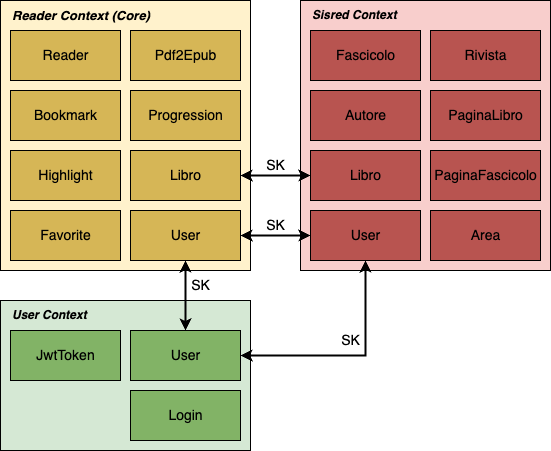
\includegraphics[width=0.7\textwidth]{img/tesi-20-app-domain.drawio.png}
\caption{Context Map: panoramica globale dei contesti del progetto e delle relazioni che intercorrono tra di essi}
\end{figure}

Tra i contesti definiti esistono delle relazioni di tipo \textit{Shared Kernel}\cite{evans_domain-driven_2004} (SK) con l'obiettivo di evitare duplicazioni e semplificare l'integrazione. Relazioni di questo tipo consistono nella condivisione di un sottoinsieme del dominio modellato, che corrisponde tipicamente al dominio core. Un esempio di relazione SK è l'utilizzo di codice o schemi DB condivisi\footnote{\url{https://github.com/ddd-crew/context-mapping}}.\\

\begin{figure}[H]
\centering
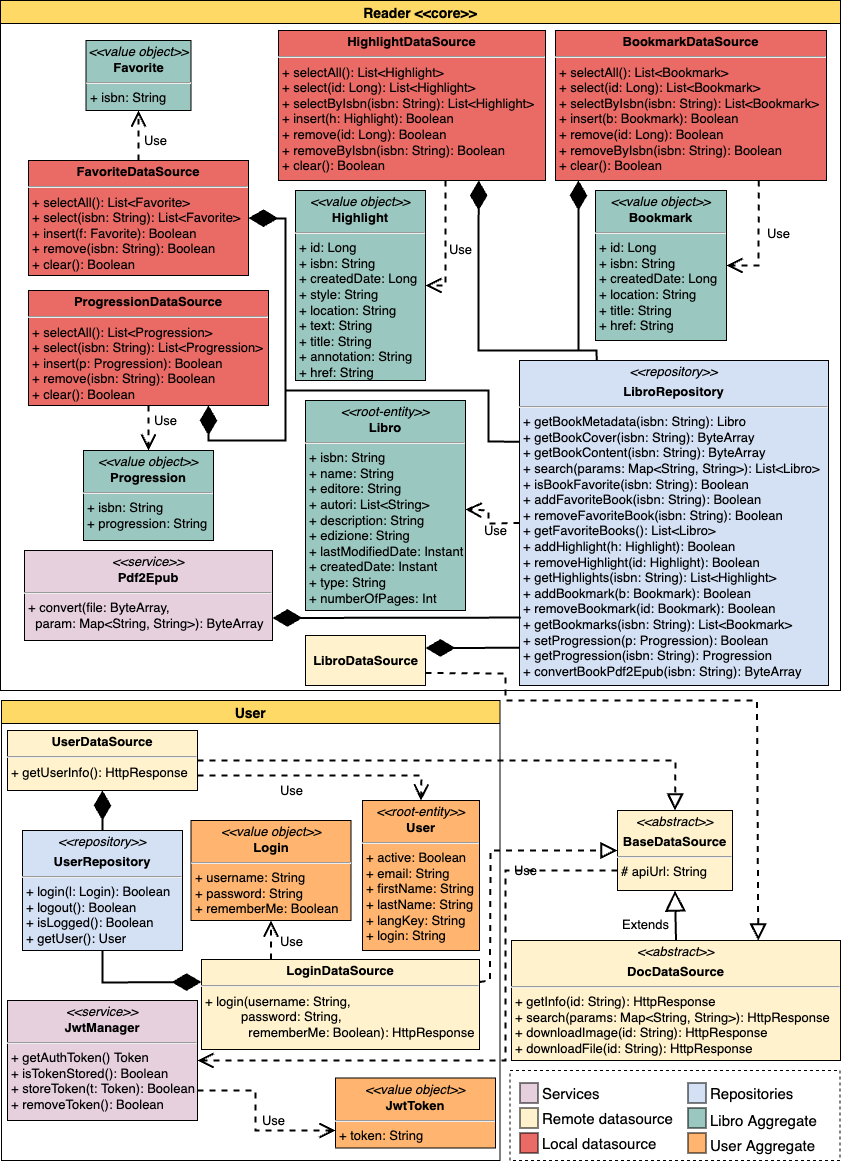
\includegraphics[width=0.9\textwidth]{img/tesi-25-ddd.drawio.png}
\caption{UML - Diagramma delle classi: Reader Core Domain e User Subdomain}
\label{fig:5.4}
\end{figure}

Per la modellazione del dominio si fa uso dei seguenti concetti\cite{evans_domain-driven_2004}:
\begin{itemize}
    \item \textit{Entity} - Oggetto definito dalla sua identità e non dai suoi attributi. Ogni libro è univoco, identificato da uno specifico codice, chiamato ISBN\footnote{International Standard Book Number}.
    \item \textit{Value Object} - Al contrario delle entità, questi oggetti sono definiti dai loro attributi e non hanno una identità concettuale ma servono a descrivere alcune caratteristiche di un oggetto. Un esempio è il segnalibro: ciò che è rilevante è la pagina del libro che esso referenzia e non la sua identità.
    \item \textit{Aggregate} - Insieme di oggetti legati da una entità padre chiamata \textit{Root} (radice di aggregazione). L'aggregato composto da \textit{Bookmark}, \textit{Highlight}, \textit{Progression}, \textit{Favorite} ha come radice l'entità \textit{Libro}.
    \item \textit{Service} - Operazione che non appartiene logicamente a nessun oggetto. In questo caso la conversione di formato non appartiene alla sola entità libro ma appartiene invece a qualsiasi documento che è possibile convertire.
    \item \textit{Repository} - Oggetto per il recupero di altri oggetti di dominio e per la gestione del loro ciclo di vita. Le entità \textit{User} e \textit{Libro} sono esempi di oggetti di dominio che necessitano di un repository. Permette di disaccoppiare applicazione e domain design dalle specifiche tecnologie/strategie di persistenza come multipli database e datasource (locali e/o remoti).
\end{itemize}

\subsection{Progettazione UX/UI}

L'interfaccia grafica della applicazione è stata progettata tramite l'utilizzo di mockup digitali realizzati con il tool grafico open source Drawio\footnote{\url{https://github.com/jgraph/drawio}}.\\
Considerando l'utilizzo tipico di una applicazione della stessa tipologia di quella che deve essere realizzata, sono stati utilizzati alcuni standard de-facto come ad esempio il menu laterale a scomparsa (mockup 4), icona "hamburger" per l'apertura del menu (mockup 3), elenco di elementi con scroll infinito verticale (schermata 2-5) e barra di ricerca nella parte alta con icona "lente di ingrandimento" (schermata 2-5).

\begin{figure}[H]
\centering
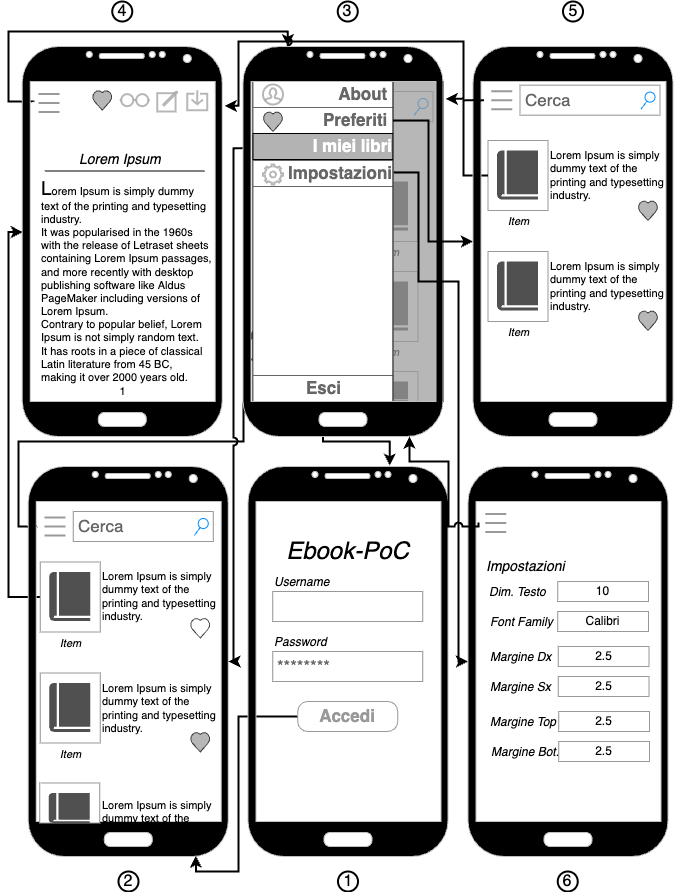
\includegraphics[width=1\textwidth]{img/tesi-14-mockup1.drawio.png}
\caption{Alcuni dei mockup realizzati per la progettazione e la validazione della UX/UI (v1)}
\end{figure}

\begin{figure}[H]
\centering
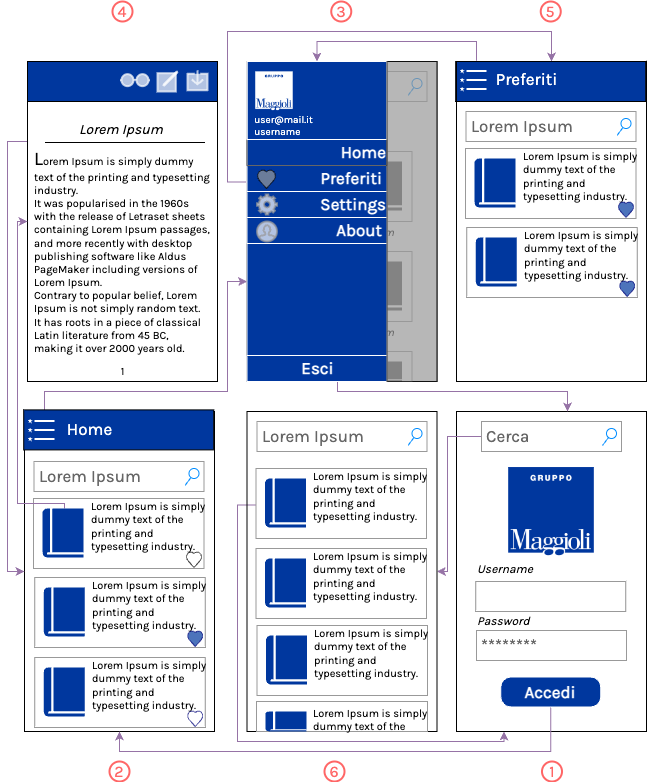
\includegraphics[width=0.95\textwidth]{img/tesi-23-mockupv2.drawio.png}
\caption{Modifiche apportate ai mockup per ottenere la validazione della UX/UI (v2)}
\end{figure}

Per ottenere la validazione dei mockup da parte degli interessati sono state necessarie due iterazioni del processo di progettazione UX/UI. L'interfaccia utente desiderata deve soddisfare alcuni vincoli caratteristici del brand Maggioli, come ad esempio l' utilizzo del colore blu \#00379E come colore primario, l'utilizzo del font Karla\footnote{\url{https://github.com/googlefonts/karla}} e la presenza del logo Maggioli. Le schermate necessarie sono quindi:
\begin{itemize}
    \item \textit{Reader} - Schermata responsabile della visualizzazione del contenuto digitale in formato EPUB.
    \item \textit{Login} - Schermata iniziale responsabile alla autenticazione dell'utente.
    \item \textit{Home} - Schermata principale responsabile alla visualizzazione dei contenuti digitali a cui l'utente è autorizzato ad accedere.
    \item \textit{Preferiti} - Schermata responsabile alla visualizzazione dei contenuti digitali preferiti dall'utente.
    \item \textit{Impostazioni} - Schermata responsabile alla visualizzazione e modifica delle impostazioni.
    \item \textit{About} - Schermata responsabile alla visualizzazione di informazioni generali come versione della applicazione, autore, copyright, ... .
\end{itemize}

\section{Implementazione}
La fase di implementazione consiste nello sviluppo della applicazione secondo il paradigma Kotlin Multiplatform: sono presenti infatti un unico core, chiamato \textit{shared} ($i$), che definisce la logica condivisa della applicazione e due differenti implementazioni per l'interfaccia utente, chiamate rispettivamente \textit{androidMaggioliEbookApp} ($ii$) e \textit{iosMaggioliEbookApp} ($iii$).

\subsection{Ricerca Librerie}
La prima attività svolta nella fase di implementazione è stata la ricerca delle librerie, la quale ha permesso di individuare le seguenti librerie, suddivise per modulo di appartenenza:
\begin{itemize}
    \item \textit{Shared}
    \begin{itemize}
        \item \textit{Ktor} - Framework asincrono per lo sviluppo di microservizi e applicazioni web. Nel progetto Ktor è utilizzato per la parte di networking come client HTTP.
        \item \textit{Kotlinx-Serialization} - Libreria multiplatform per la serializzazione dei dati.
        \item \textit{Kotlinx-Datetime} - Libreria multiplatform per la gestione delle date e del tempo.
        \item \textit{Kvault}\footnote{\url{https://github.com/Liftric/KVault}} - Libreria multiplatform per la persistenza dei dati sicura in formato chiave-valore. Tramite una unica API si comporta come wrapper di Keychain, nel caso iOS, e SharedPreferences nel caso Android.
        \item \textit{Koin}\footnote{\url{https://github.com/InsertKoinIO/koin}} - Dependency Injection framework multiplatform.
        \item \textit{Napier}\footnote{\url{https://github.com/AAkira/Napier}} - Logging framework multiplatform.
        \item \textit{SqlDelight}\footnote{\url{https://github.com/cashapp/sqldelight}} - Libreria multiplatform per la persistenza dei dati tramite database relazionale locale.
    \end{itemize}
    \item \textit{Android}
    \begin{itemize}
    \item \textit{Readium} (Kotlin-toolkit)\footnote{\url{https://github.com/readium/kotlin-toolkit}} - Libreria per la manipolazione e visualizzazione di contenuti editoriali digitali. Implementazione specifica per la piattaforma Android. 
    \end{itemize}
    \item \textit{iOS}
    \begin{itemize}
    \item \textit{Readium} (Swift-toolkit)\footnote{\url{https://github.com/readium/swift-toolkit}} - Libreria per la manipolazione e visualizzazione di contenuti editoriali digitali. Implementazione specifica per la piattaforma iOS. 
    \item \textit{KMPNativeCoroutines}\footnote{\url{https://github.com/rickclephas/KMP-NativeCoroutines}} - Libreria che permette l'utilizzo delle coroutine Kotlin in Swift in applicazioni Kotlin Multiplatform.
    \end{itemize}
\end{itemize}
Per ognuna delle librerie del modulo \textit{Shared} esistono valide alternative, dimostrando che l'ecosistema Kotlin Multiplatform è in continua espansione\footnote{\url{https://github.com/terrakok/kmm-awesome}}.

\subsection{Readium}
Le uniche due librerie individuate che da documentazione sono in grado di rispettare i requisiti di gestione, manipolazione e visualizzazione dei contenuti digitali in formato EPUB sono \textit{Readium}\footnote{\url{https://github.com/readium}} e \textit{FolioReader}\footnote{\url{https://github.com/FolioReader}}.\\
Entrambe le librerie forniscono le stesse identiche funzionalità ma è stata scelta \textit{Readium} come libreria per la applicazione per le seguenti motivazioni:
\begin{itemize}
    \item Non è stato possibile testare la libreria \textit{FolioReader} a causa di errori al suo interno in fase di compilazione della applicazione di test realizzata.
    \item Per la libreria \textit{Readium} l'ultima commit per la versione Android risale al 05/09/2022 e l'ultimo rilascio risale al 22/04/2022, mentre per la libreria \textit{FolioReader} l'ultima commit per la versione Android risale al 09/01/2020 e l'ultimo rilascio risale al 11/01/2019. Lo stesso confronto è valido per la versione iOS.\footnote{Dati al 06/09/2022 provenienti dai relativi repository GitHub}
    \item La libreria \textit{Readium} è scritta con il linguaggio Kotlin mentre \textit{FolioReader} è scritta con Java.
\end{itemize}
La necessità di un tool open-source, robusto e performante per la manipolazione e la lettura di formati editoriali digitali è alla base del progetto Readium. Essa infatti consiste in un insieme di toolkit per diversi formati (come epub, audiolibri e libri image-based) e diverse piattaforme (Android, iOS, Desktop e Web).\\
L'architettura della libreria \textit{Readium} è cosi composta da quattro moduli principali:
\begin{itemize}
    \item \textit{Publication Server} - Fornisce le pubblicazioni tramite un server locale HTTPS.
    \item \textit{Streamer} - Modulo composto dai seguenti due sottomoduli:
    \begin{itemize}
        \item \textit{Parser} - Responsabile del parsing delle pubblicazioni e della loro esposizione utilizzando un modello in-memory.
        \item \textit{Fetcher} - Si occupa di ottenere i contenuti delle pubblicazioni e della loro manipolazione (in particolare injection di CSS e Javascript nelle risorse HTML).
    \end{itemize}
    \item \textit{Navigator} - Utile alla navigazione delle risorse di una pubblicazione secondo diverse strategie basate sulla natura della pubblicazione (ebook, audiolibri, ...). Interagisce con il modulo \textit{Streamer} per utilizzare il modello in-memory o per ottenere manifesto JSON attraverso il modello condiviso (\textit{Shared}).
\end{itemize}
\begin{figure}[H]
\centering
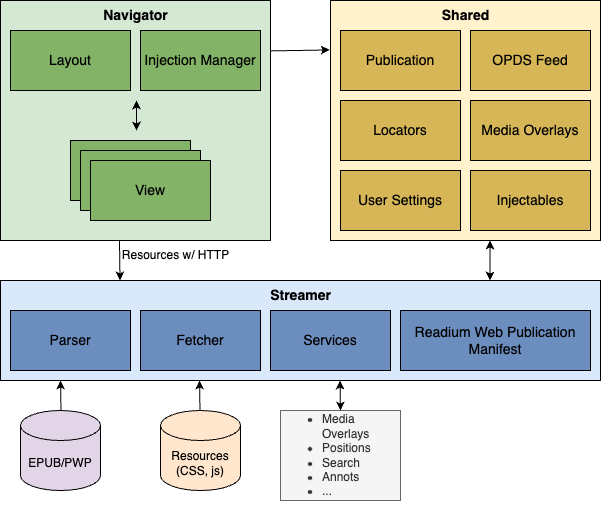
\includegraphics[width=0.7\textwidth]{img/tesi-22-readiumarch.drawio.png}
\caption{Architettura libreria Readium}
\label{readiumarch}
\end{figure}

\subsection{Shared}
Come anticipato nel capitolo \ref{ch:ch3} la parte condivisa della applicazione racchiude tutta o una sottoparte della business logic, compresi quindi aspetti "infrastrutturali" specifici della piattaforma target come ad esempio logging, persistenza dei dati e networking. E' infatti in questo modulo che si trova l'implementazione della logica applicativa seguendo le specifiche definite in fase di progettazione (figura \ref{fig:5.4}).\\
Lo schema del database locale è definito utilizzando appositi file, in formato \textit{.sq}, uno per ognuna delle entità che necessita di persistenza: \textit{Highlight}, \textit{Favorite}, \textit{Progression} e \textit{Bookmark}. Tramite il task \textit{generateSqlDelightInterface} fornito dal plugin gradle SqlDelight è possibile generare le relative implementazioni dell'interfaccia \textit{MaggioliEbookDB}, anch'essa autogenerata dal plugin. 

\begin{figure}[H]
\centering
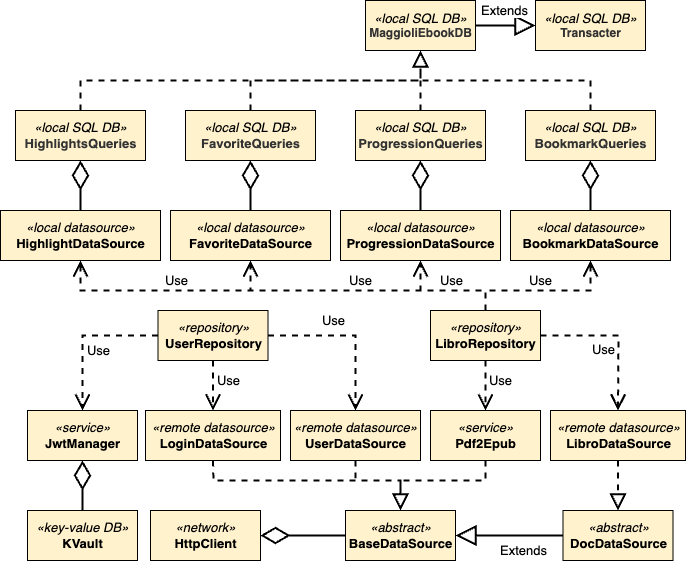
\includegraphics[width=1\textwidth]{img/tesi-26-shareduml.drawio.png}
\caption{UML - Diagramma delle classi: Implementazioni data source (persistenza dati e networking)}
\end{figure}

\begin{listing}[H]
\inputminted{sql}{code/5-sqldelight}
\caption{Esempio di definizione schema \textit{Bookmark} tramite sintassi SqlDelight}
\end{listing}

\begin{listing}[H]
\inputminted{kotlin}{code/5-sqldelight1}
\caption{Implementazione autogenerata tramite il plugin gradle SqlDelight della precedente definizione dello schema per l'entità \textit{Bookmark}}
\end{listing}

Tipicamente le librerie per applicazioni sviluppate con Kotlin Multiplatform possono essere utilizzate direttamente dal codice condiviso, come ad esempio KVault, lasciando al compilatore Kotlin il compito di scegliere la giusta implementazione per la piattaforma target durante la fase di compilazione.In altri casi è necessario invece utilizzare il meccanismo \textit{expect/actual} (discusso nel capitolo \ref{ch:ch3}) per definire il comportamento atteso e fornire una implementazione specifica per la piattaforma target.\\
Tale meccanismo è stato utilizzato nello sviluppo della applicazione per poter effettuare dependency injection tramite la libreria Koin dei componenti riguardanti la persistenza dei dati (Kvault e SqlDelight) e l'esecuzione asincrona (CoroutineDispatcher).

\begin{figure}[H]
\centering
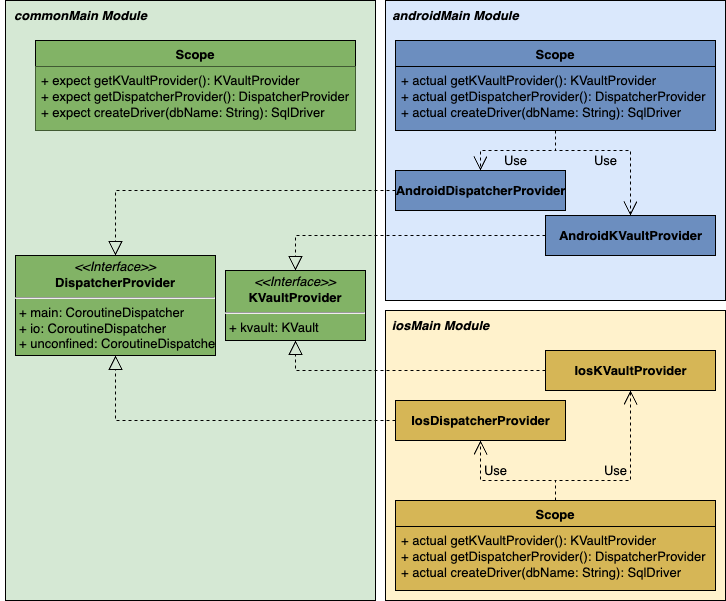
\includegraphics[width=0.9\textwidth]{img/tesi-21-expectactual.drawio.png}
\caption{Strategia \textit{Expect/Actual} adottata per l'implementazione dei servizi infrastrutturali specifici delle piattaforme, persistenza e concorrenza, sfruttando la tecnica \textit{dependency injection}}
\end{figure}

Ogni dipendenza che deve essere iniettata viene inserita all'interno di uno o più moduli, i quali vengono utilizzati da Koin per inizializzare tutto il contesto applicativo. Le dipendenze possono essere principalmente di due tipi:
\begin{itemize}
    \item \textit{Factory} - Ogni volta che la dipendenza viene iniettata ne viene creata una nuova istanza (paragonabile al design pattern Factory Method\footnote{\url{https://en.wikipedia.org/wiki/Factory_method_pattern}}).
    \item \textit{Single} - In tutto il contesto applicativo esiste una sola istanza della dipendenza iniettata (paragonabile al design pattern Singleton\footnote{\url{https://en.wikipedia.org/wiki/Singleton_pattern}}).
\end{itemize}

\begin{listing}[H]
\inputminted{kotlin}{code/5-koin}
\caption{Configurazione Dependency Injection: definizione dei moduli Koin e inizializzazione del contesto applicativo}
\end{listing}

\subsection{androidMaggioliEbookApp}
L'applicazione sviluppata per la piattaforma Android implementa sia lo strato della visualizzazione dei dati utilizzando la business logic fornita dal modulo \textit{Shared} che la logica del \textit{Reader}, lettore dei contenuti digitali realizzato tramite il toolkit Kotlin della libreria \textit{Readium}.
\subsubsection{Single-Activity Architecture}
L'architettura scelta per l'implementazione della applicazione Android è basata su sole due activity:
\begin{itemize}
    \item \textit{MainActivity} - Unica activity principale della applicazione.
    \item \textit{ReaderActivity} - Activity secondaria, utilizzata sia per l'interazione che la gestione del lettore di contenuti digitali.
\end{itemize}
Questa tipologia di architettura permette di avere una singola activity che svolge la funzione di "big container" per tutti i fragment che rappresentano le varie schermate della applicazione.

\begin{figure}[H]
\centering
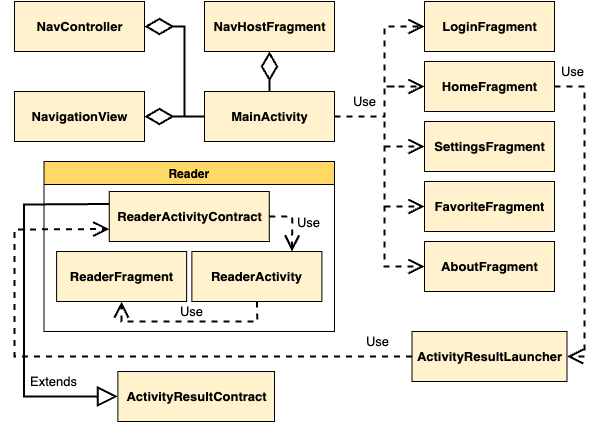
\includegraphics[width=0.7\textwidth]{img/tesi-27-singleactivity.drawio.png}
\caption{UML - Diagramma delle classi: architettura Single-Activity}
\label{fig:5.10}
\end{figure}

La navigazione all'interno della applicazione è gestita tramite la combinazione dei seguenti componenti:
\begin{itemize}
    \item \textit{NavController} - Componente necessario per la gestione delle transizioni da un un fragment all'altro. Quando inizializzato richiede la presenza di un grafo di navigazione tra le risorse XML: tale grafo contiene tutti i fragment che possono essere visualizzati e le possibili transizioni tra di essi.
    \item \textit{NavHostFragment} - Rappresenta il contenitore del fragment in cui ci si trova. Ogni transizione nel grafo corrisponde alla sostituzione del fragment visualizzato con quello di destinazione (sempre che la transizione sia ammessa dal grafo).
    \item \textit{NavigationView} - Permette la visualizzazione del menu dove si trovano i possibili fragment raggiungibili da quello in cui l'utente si trova attualmente. Nel caso della applicazione sviluppata in questo componente si trova il menu laterale con tutte le schermate indicate in fase di progettazione (\textit{Home}, \textit{Settings}, \textit{About} e \textit{Preferiti}).
\end{itemize}

\begin{figure}[H]
\centering
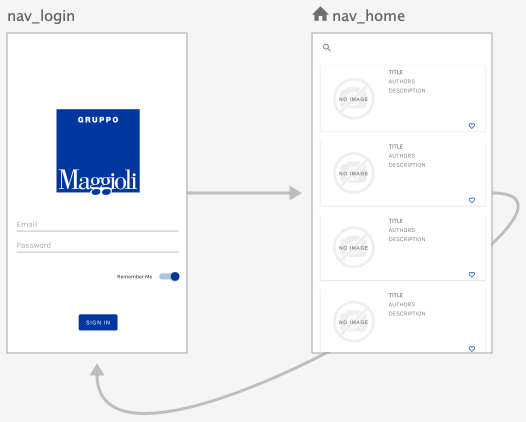
\includegraphics[width=0.7\textwidth]{img/Screenshot 2022-09-20 at 08.26.21.png}
\caption{Screenshot di una sottoparte del navigation graph (renderizzato automaticamente tramite l'IDE Android Studio)}
\label{fig:5.11}
\end{figure}

Come indicato nella figura \ref{fig:5.11} la schermata principale (\textit{Home}) rappresenta la destinazione iniziale del grafo, ovvero la prima schermata che viene visualizzata dalla applicazione. L'autenticazione dell'utente è gestita tramite la navigazione condizionale\footnote{\url{https://developer.android.com/guide/navigation/navigation-conditional}}. Prima di creare la vista del fragment viene effettuato un controllo sulla autenticazione dell'utente: se l'utente non è autenticato viene effettuata una transizione al fragment \textit{Login} per permettere all'utente di autenticarsi e procedere all'utilizzo della applicazione. E' fondamentale in questo scenario ripulire lo stack di navigazione per evitare che l'utente possa tornare indietro alla schermata precedente, ovvero la schermata principale, senza effettuare l'autenticazione.\\

\subsubsection{Paging}
Un altro aspetto importante della architettura è il meccanismo utilizzato sia dalla schermata principale che da quella dei preferiti per mostrare i dati all'utente. Il backend utilizzato fornisce i dati tramite paginazione: in questo modo è possibile indicare in una richiesta la dimensione delle pagine, ovvero quanti elementi devono essere restituiti al massimo in una pagina, e la pagina desiderata. Per poter caricare tali dati dinamicamente in una \textit{RecyclerView}\footnote{\url{https://developer.android.com/reference/kotlin/androidx/recyclerview/widget/RecyclerView}} in modo che l'utente possa effettuare lo scroll illimitato nella schermata si utilizza la libreria \textit{Paging}\footnote{\url{https://developer.android.com/topic/libraries/architecture/paging/v3-overview}} fornita da Android.

\begin{figure}[H]
\centering
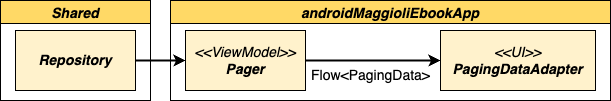
\includegraphics[width=0.75\textwidth]{img/tesi-2-Page-11.drawio.png}
\caption{Flusso generico dei dati dalla sorgente alla UI tramite l'utilizzo della libreria Paging}
\label{paging}
\end{figure}

% aggiungere materiale su paging ecc

I componenti fondamentali della libreria \textit{Paging} sono:
\begin{itemize}
    \item \textit{Pager} - Punto di ingresso principale della libreria con il compito di ottenere nuovi dati quando necessario, ovvero quando l'utente ha scrollato nella schermata fino ad uno specifico punto. Richiede la configurazione di alcuni parametri come la dimensione della pagina, la pagina iniziale e la direzione della paginazione. 
    \item \textit{PagingSource} - Sorgente dei dati paginati. Componente interrogato dal \textit{Pager} ogni volta che sono necessari nuovi dati.
    \item \textit{PagingDataAdapter} - Componente fondamentale per la rappresentazione di dati paginati in una \textit{RecyclerView}.
\end{itemize}

\begin{figure}[H]
\centering
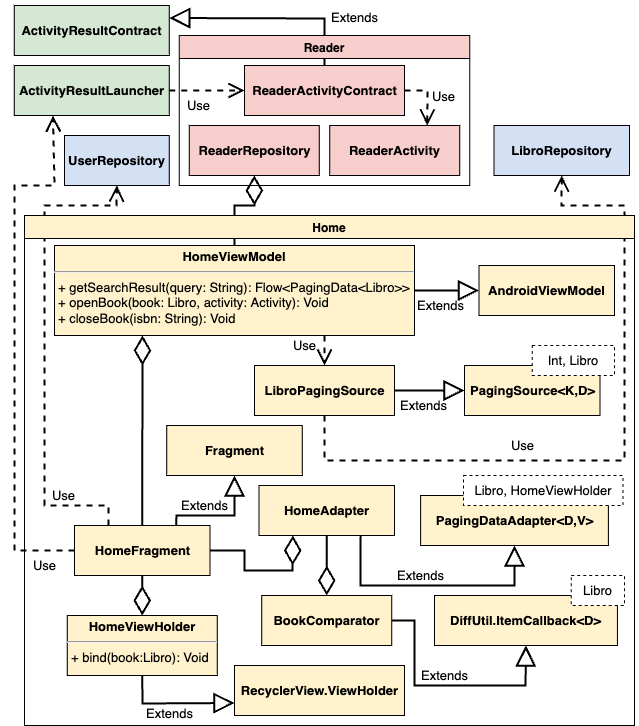
\includegraphics[width=0.7\textwidth]{img/tesi-24-androidviewuml.drawio.png}
\caption{UML - Diagramma delle classi: Paginazione dati nella schermata principale}
\label{paging2}
\end{figure}

\subsubsection{Reader}
Il lettore dei documenti digitali in formato EPUB rappresenta la funzionalità core della applicazione sviluppata. Nel caso della interfaccia grafica android il lettore riceve il contenuto da visualizzare del documento selezionato dall'utente e lo mostra in un fragment basato sul componente \textit{Navigator} (figura \ref{readiumarch}). Questo componente della libreria Readium fornisce tutte le funzionalità necessarie per gestire la navigazione dei documenti e gli eventi relativi al comportamento dell'utente come scorrimento pagine e selezione testo. \\
I principali componenti del reader sono:
\begin{itemize}
    \item \textit{ReaderActivity} - Unica activity presente nella applicazione oltre a quella principale (Single Activity Architecture), utilizzata sia per l’interazione che la gestione del lettore di contenuti digitali.
    \item \textit{EpubReaderFragment} - Componente che si occupa effettivamente di mostrare il contenuto del documento all'utente.
    \item \textit{DecorationListener} - Permette la gestione grafica delle annotazioni come evidenziazioni e sottolineature, le quali sono aggiunte alla vista del fragment tramite l'utilizzo di Jetpack Compose.
\end{itemize}

\begin{figure}[H]
\centering
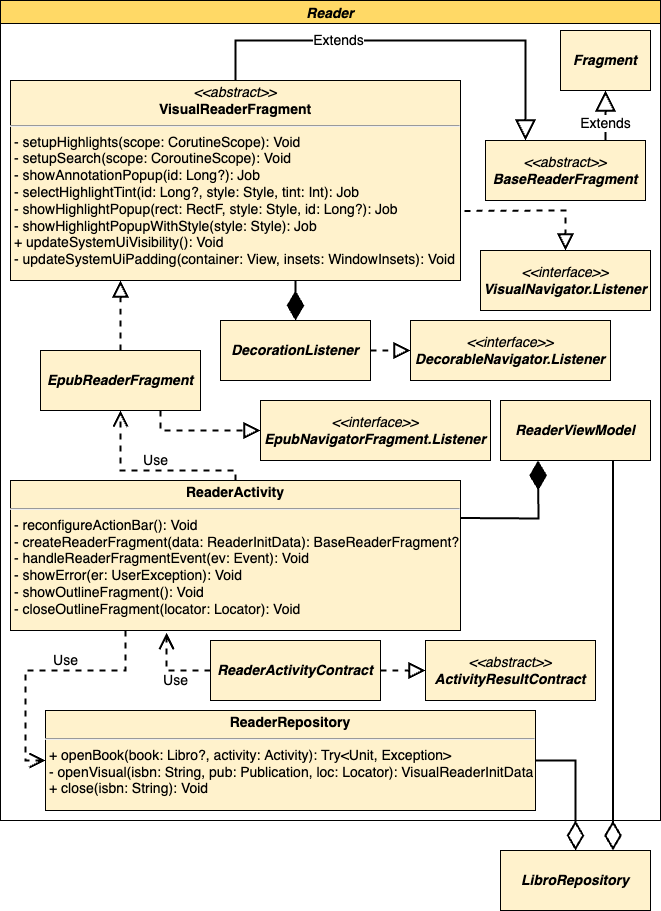
\includegraphics[width=0.8\textwidth]{img/tesi-2-Page-16.drawio.png}
\caption{UML - Diagramma delle classi: Reader}
\label{reader}
\end{figure}

\subsubsection{Screenshots}

\begin{multicols}{3}
            \begin{figure}[H]
                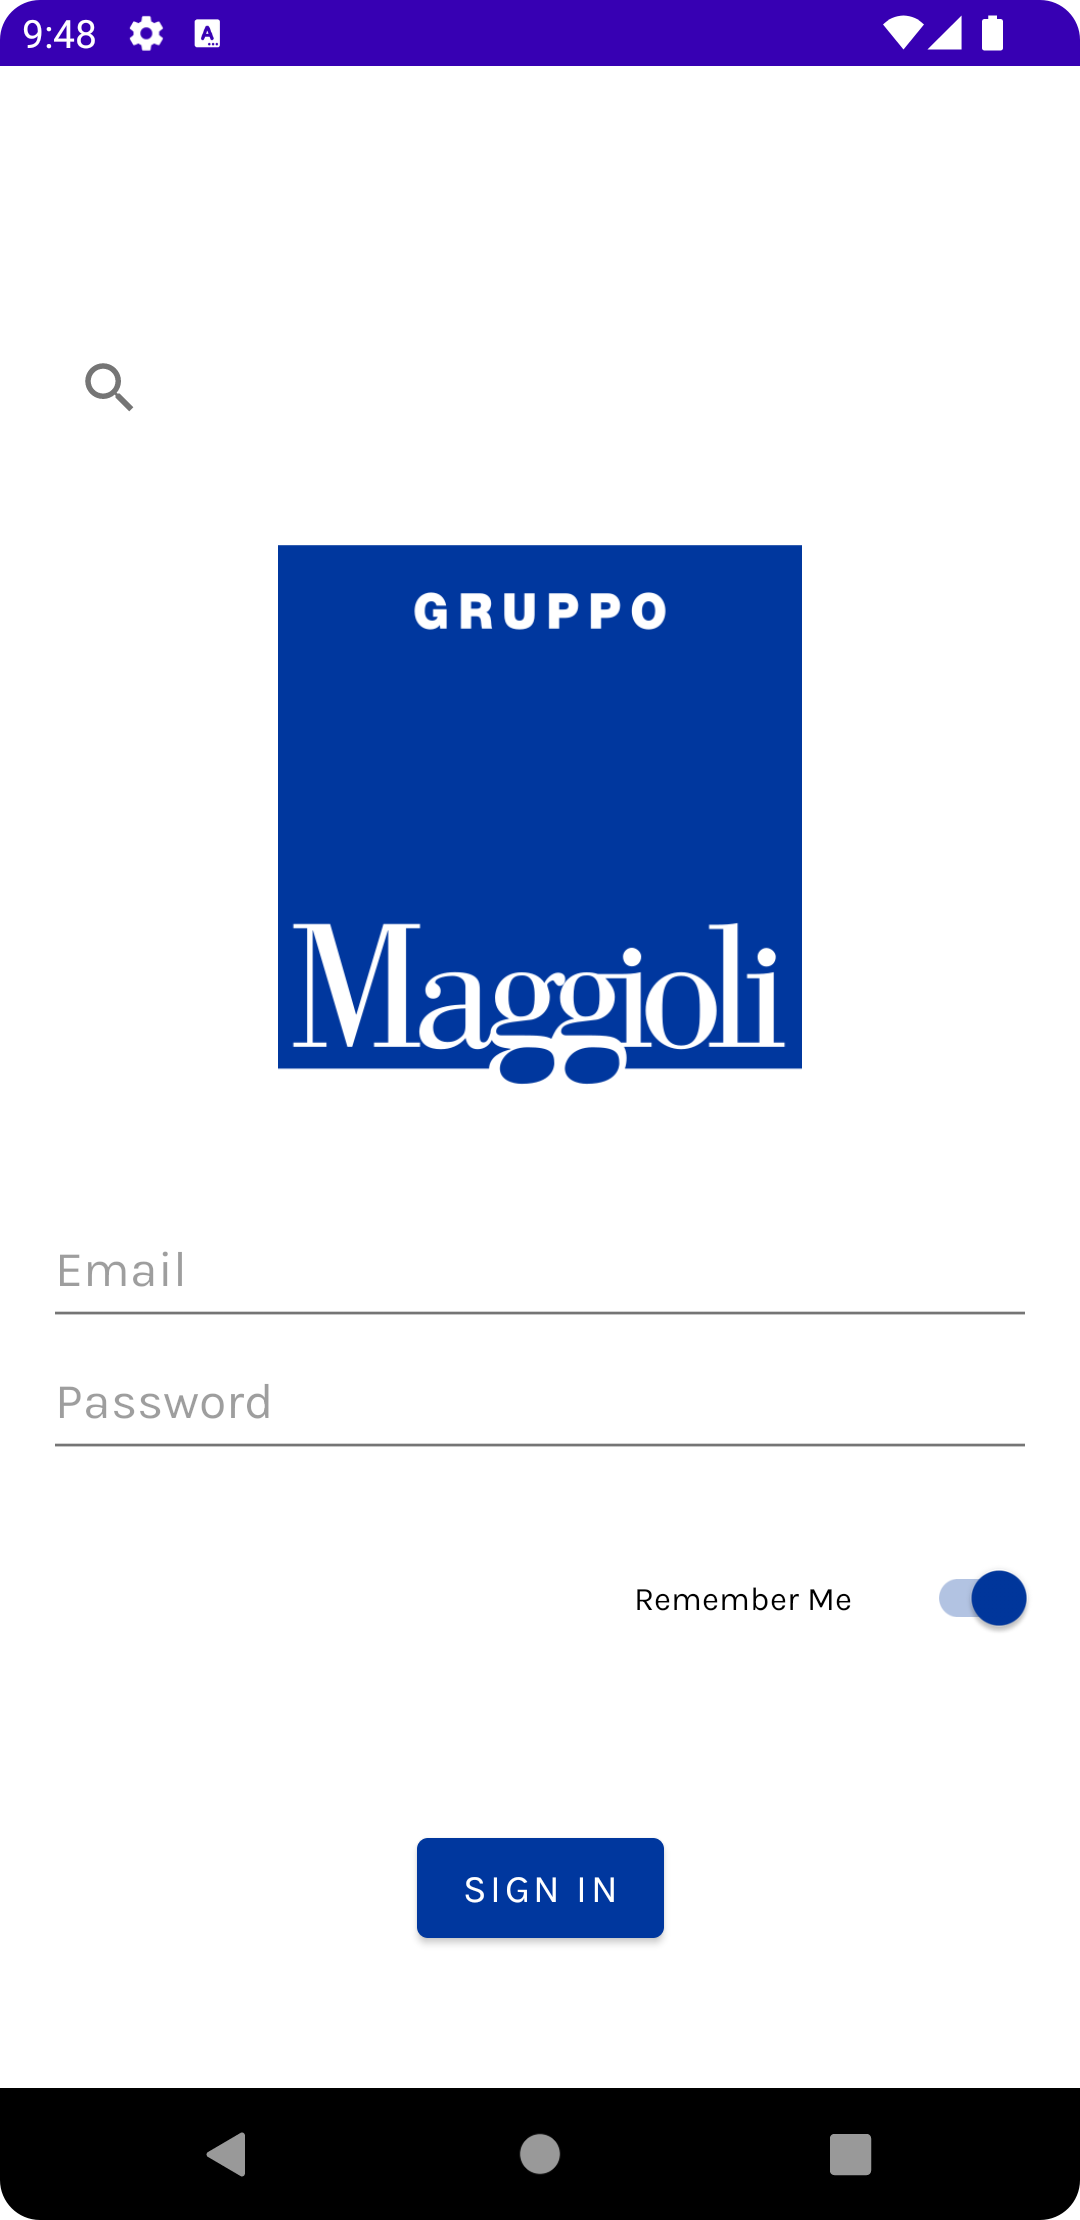
\includegraphics[width=0.21\textwidth]{img/login.png}
                \caption{Schermata di login degli utenti abbonati}
                \label{login}
            \end{figure}

            \begin{figure}[H]
                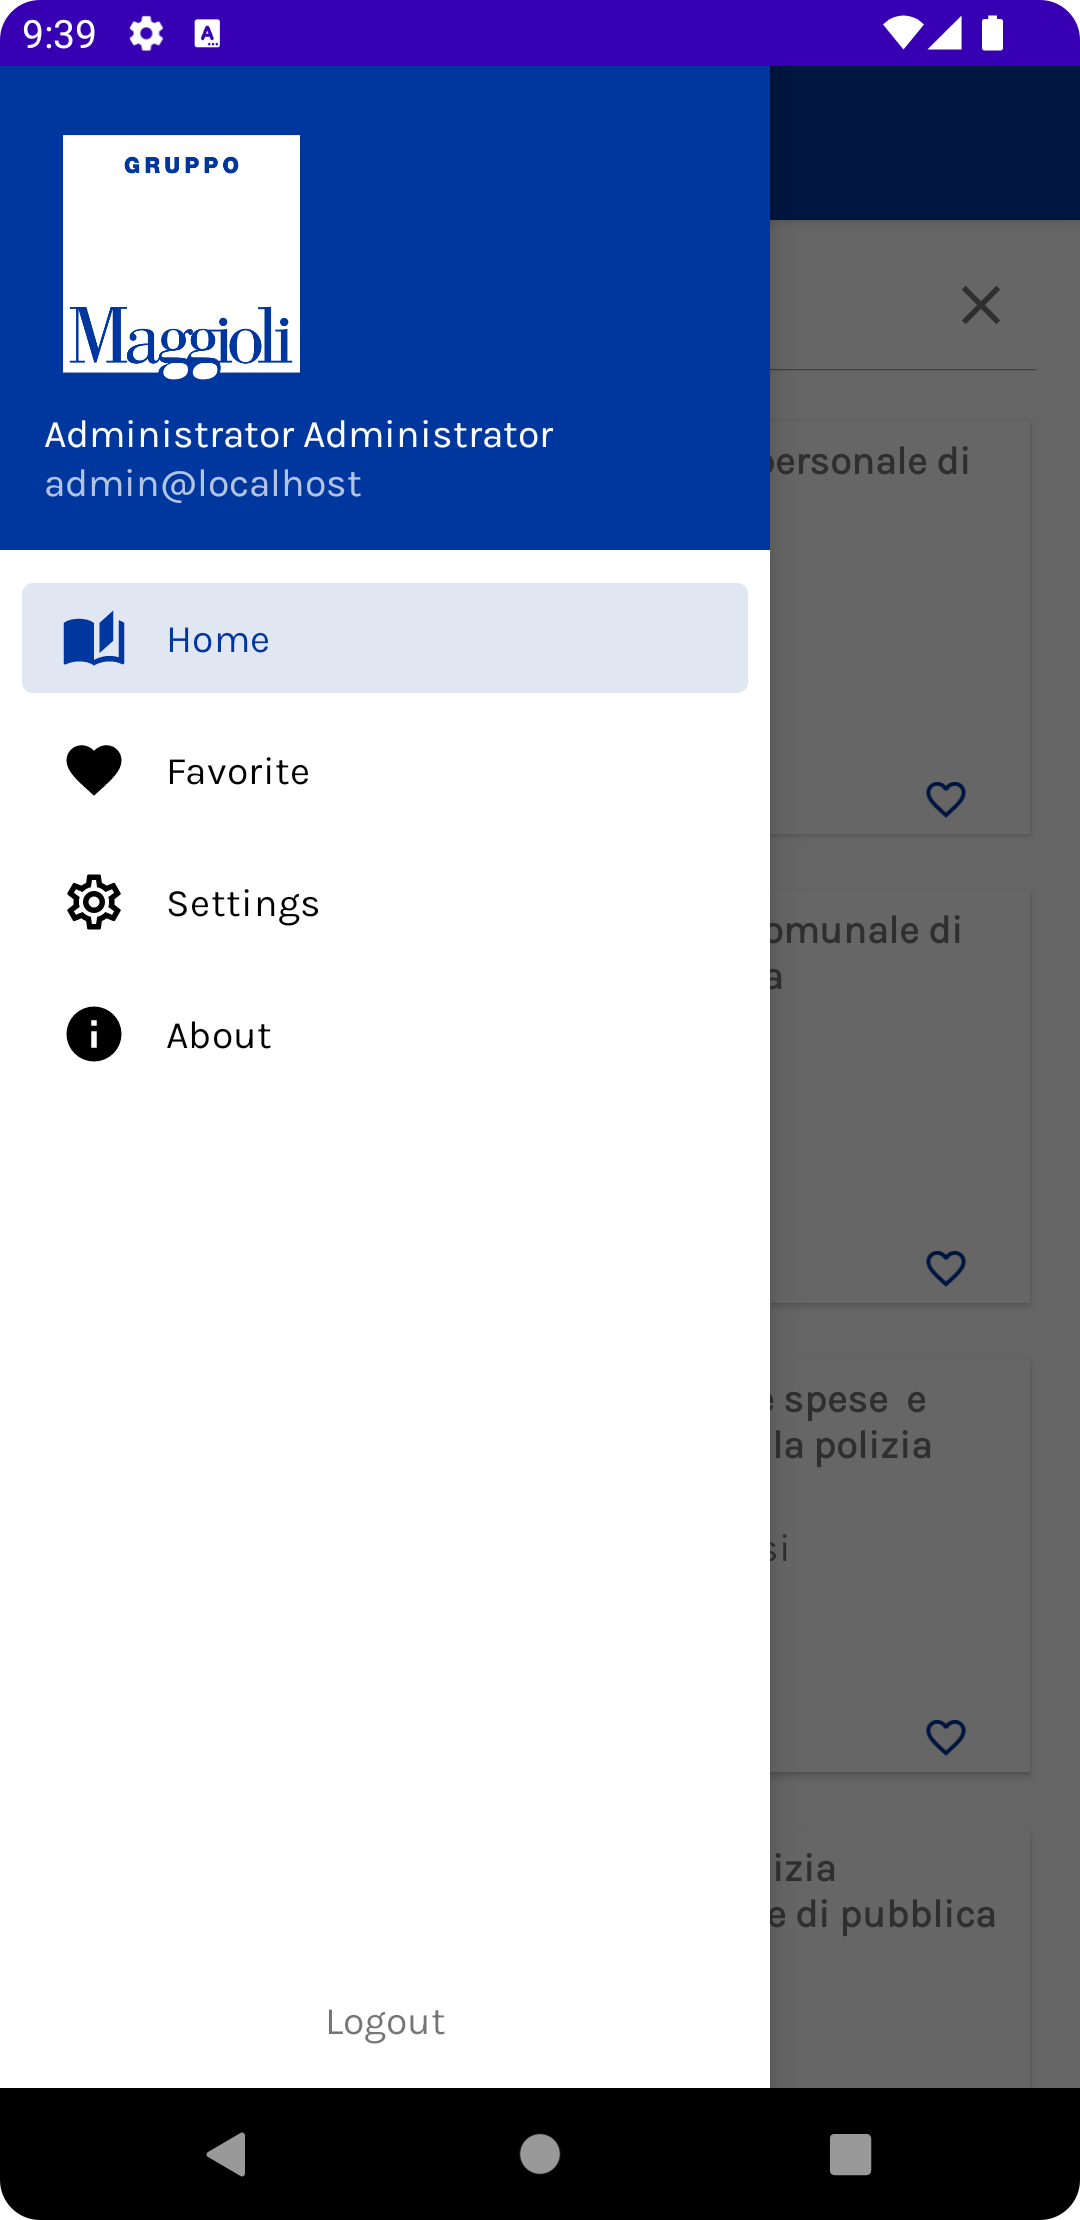
\includegraphics[width=0.21\textwidth]{img/sidenav.png}
                \caption{Menu laterale per la navigazione all'interno della applicazione}
                \label{sidenav}
            \end{figure}
            
            \begin{figure}[H]
                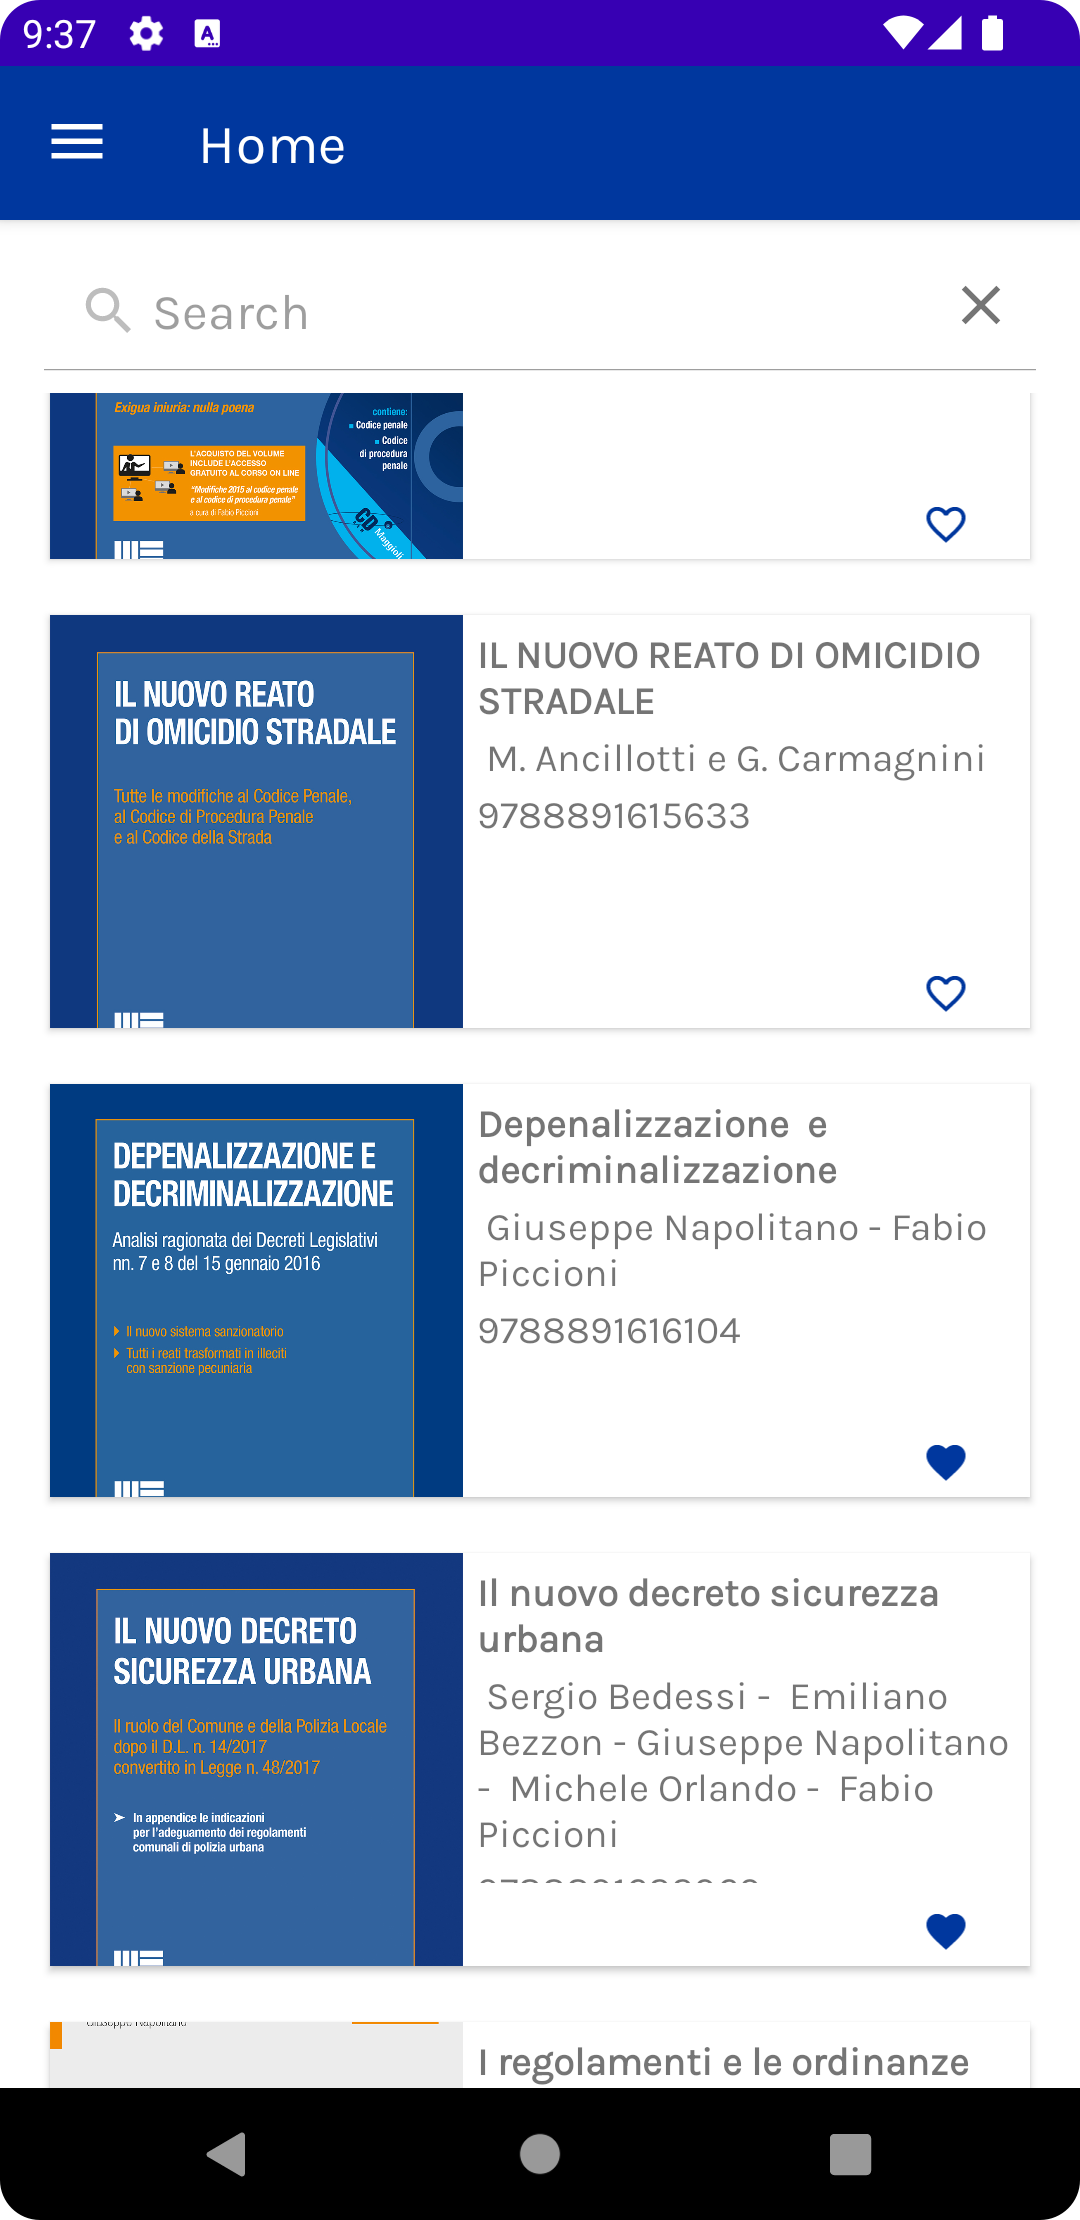
\includegraphics[width=0.21\textwidth]{img/home.png}
                \caption{Schermata home principale per la visualizzazione e la ricerca dei documenti digitali Maggioli}
                \label{home}
            \end{figure}
            
            \begin{figure}[H]
                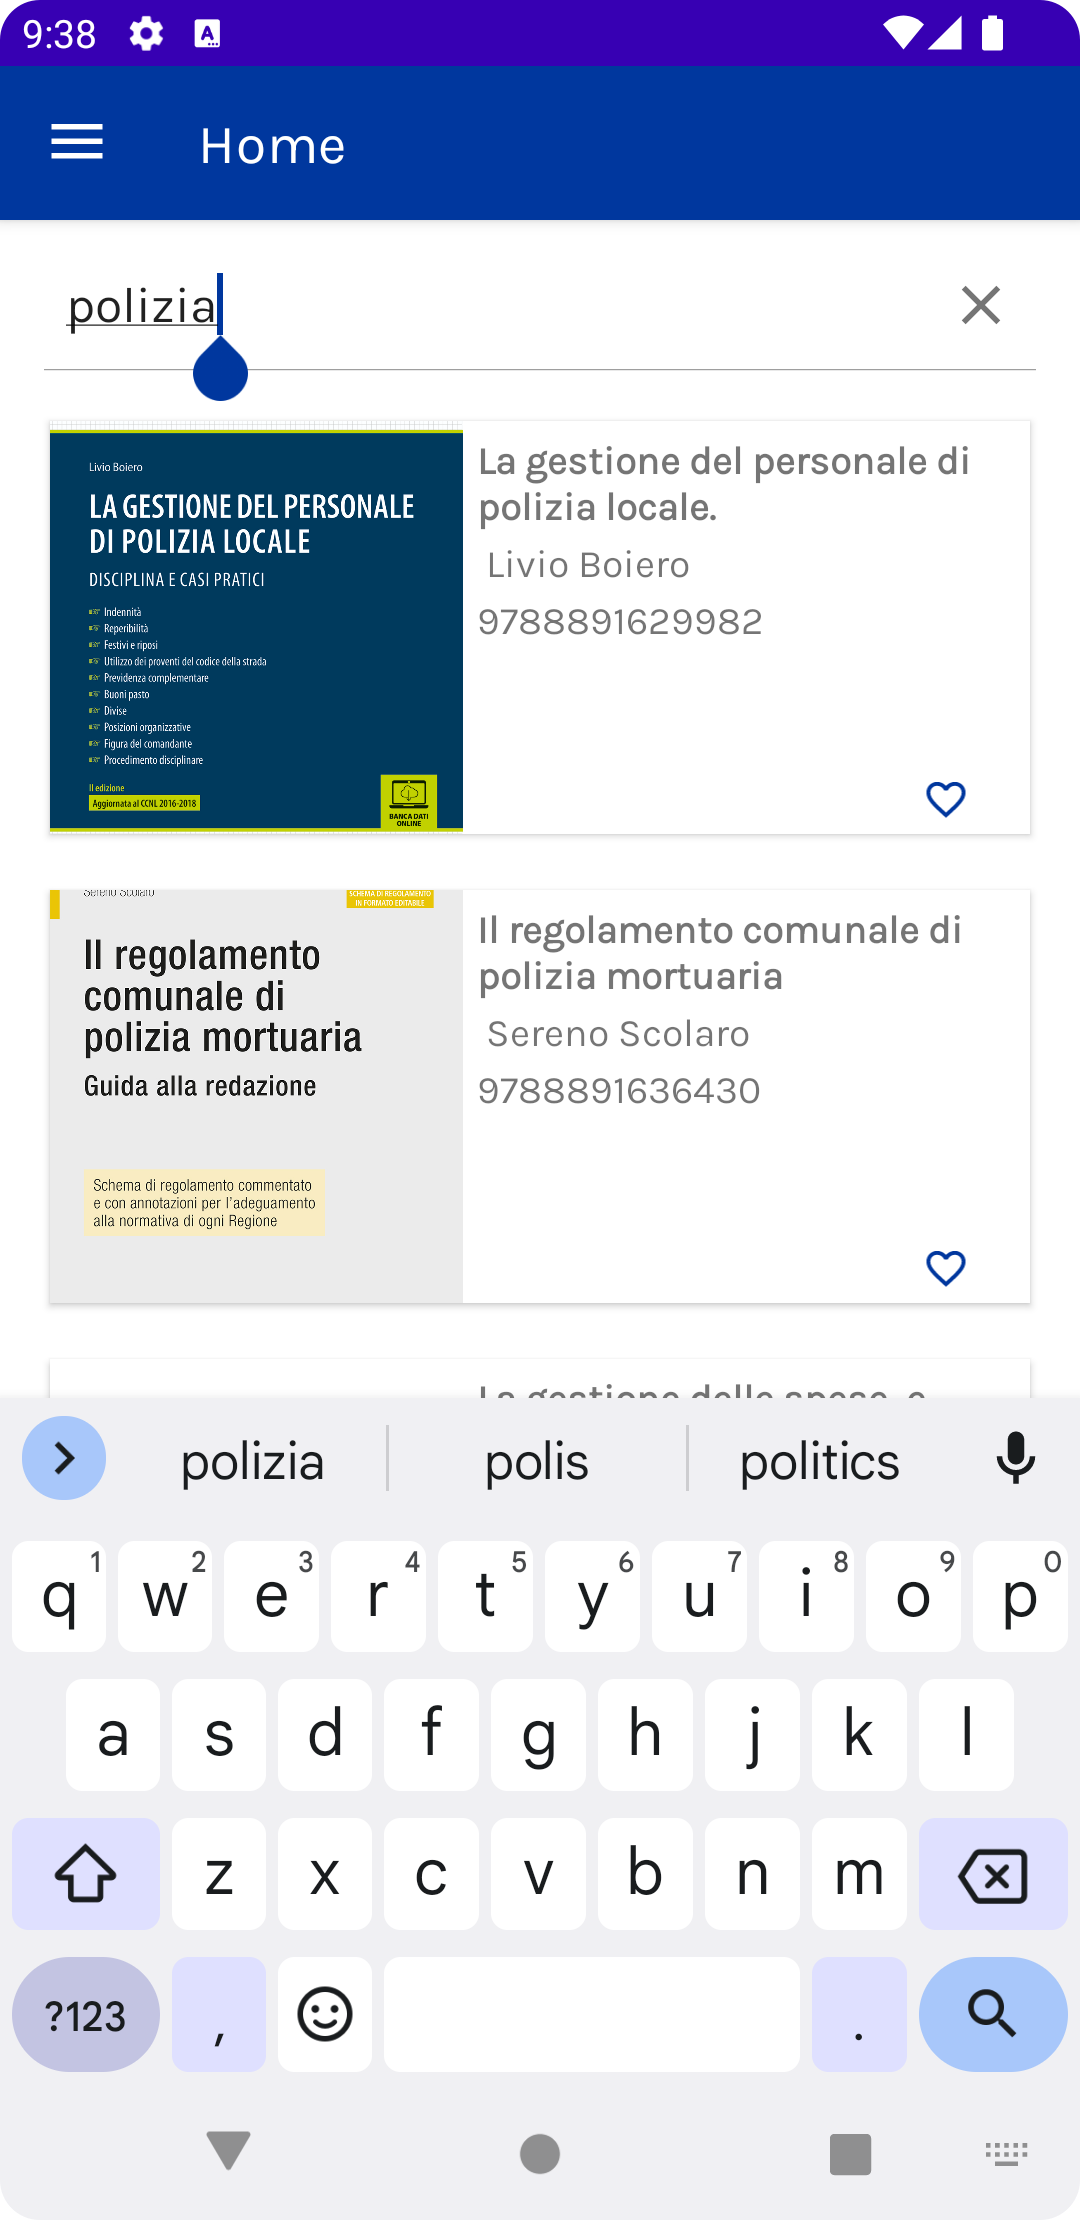
\includegraphics[width=0.21\textwidth]{img/ricerca.png}
                \caption{Esempio di ricerca per parola chiave nella schermata principale}
                \label{ricerca}
            \end{figure}

            \begin{figure}[H]
                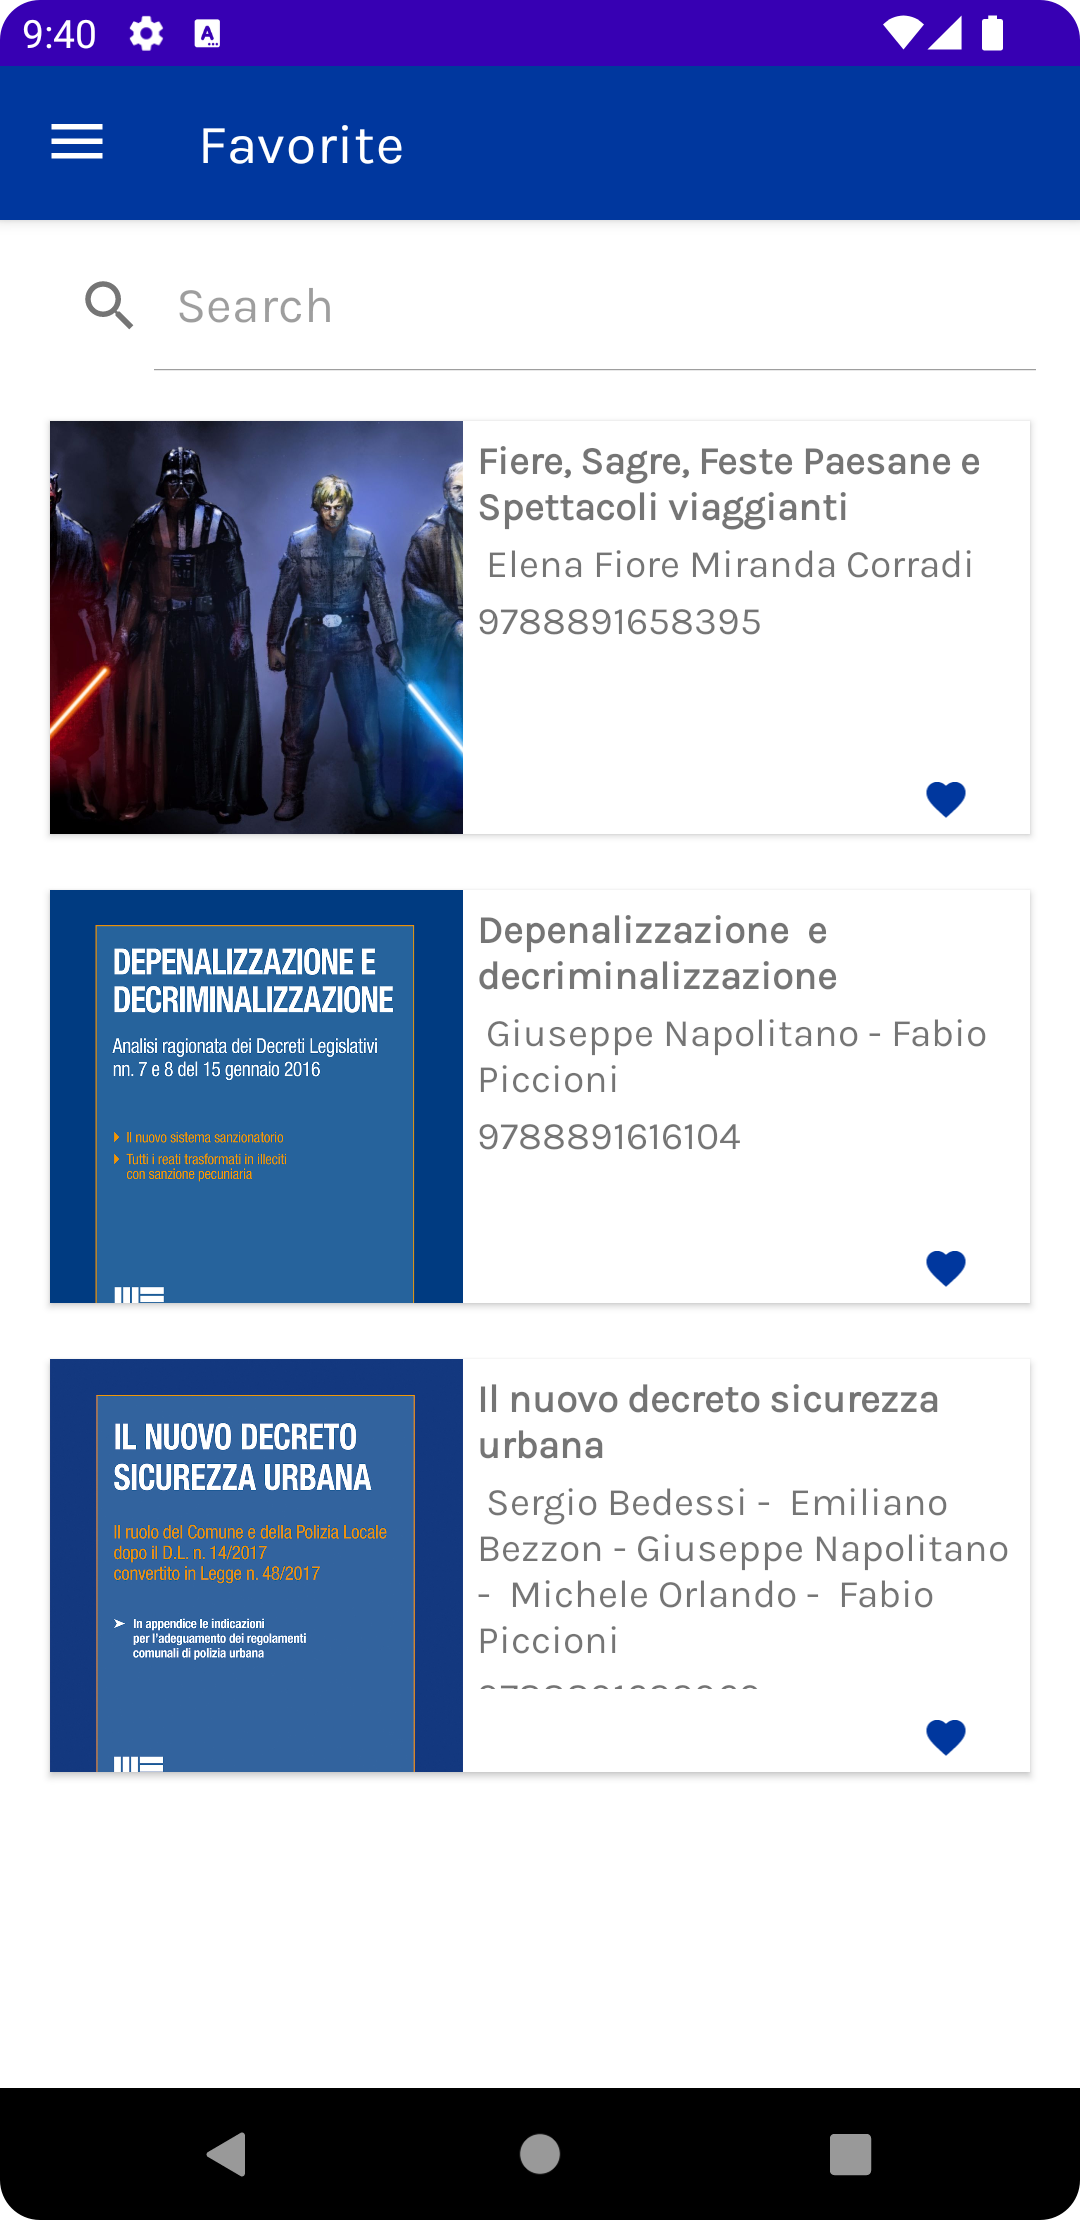
\includegraphics[width=0.21\textwidth]{img/preferiti.png}
                \caption{Schermata per la visualizzazione e la ricerca dei documenti preferiti dall'utente}
                \label{preferiti}
            \end{figure}

            \begin{figure}[H]
                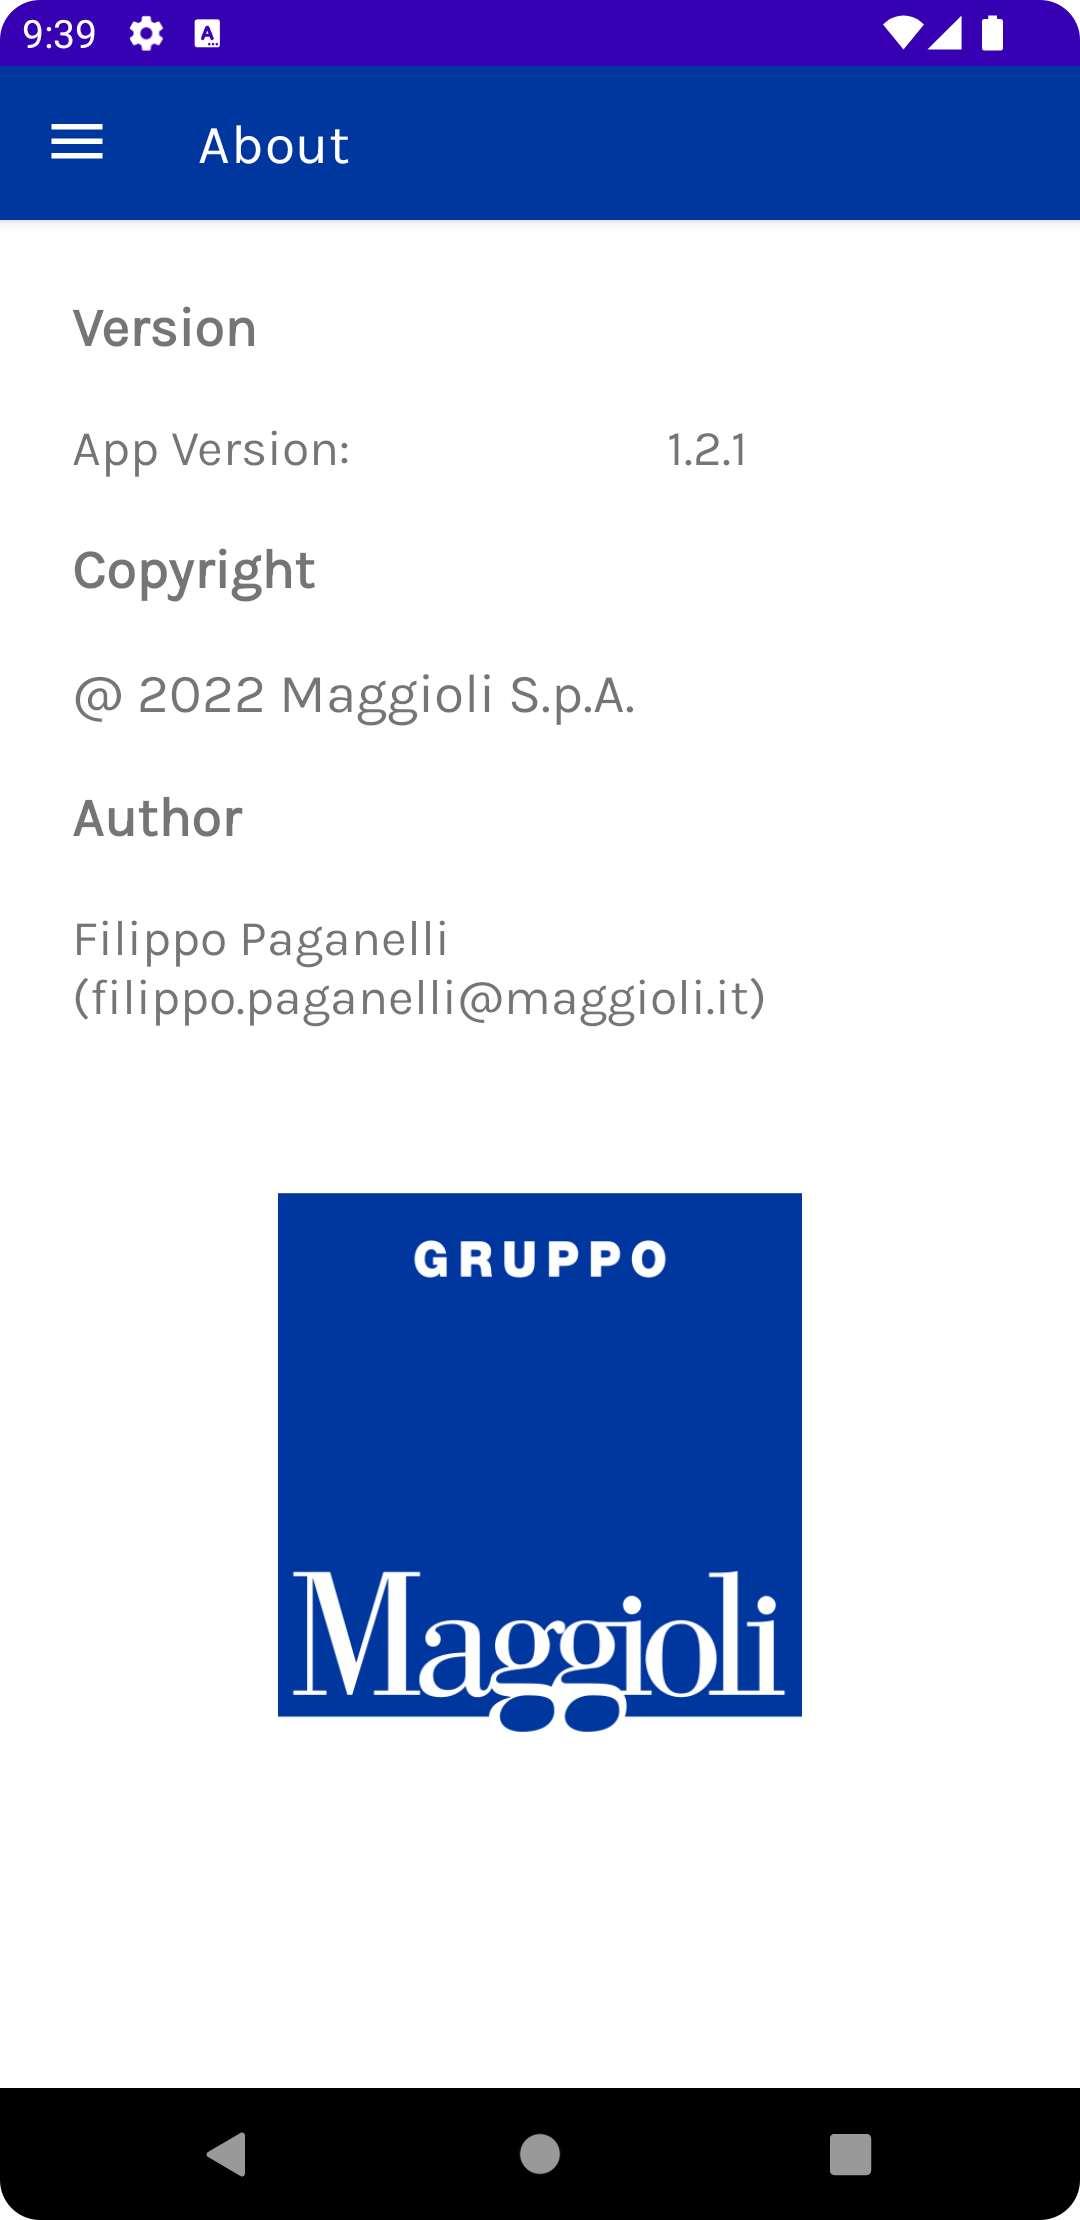
\includegraphics[width=0.21\textwidth]{img/about.png}
                \caption{Schermata per la visualizzazione delle informazioni generali relative alla applicazione}
                \label{about}
            \end{figure}

            \begin{figure}[H]
                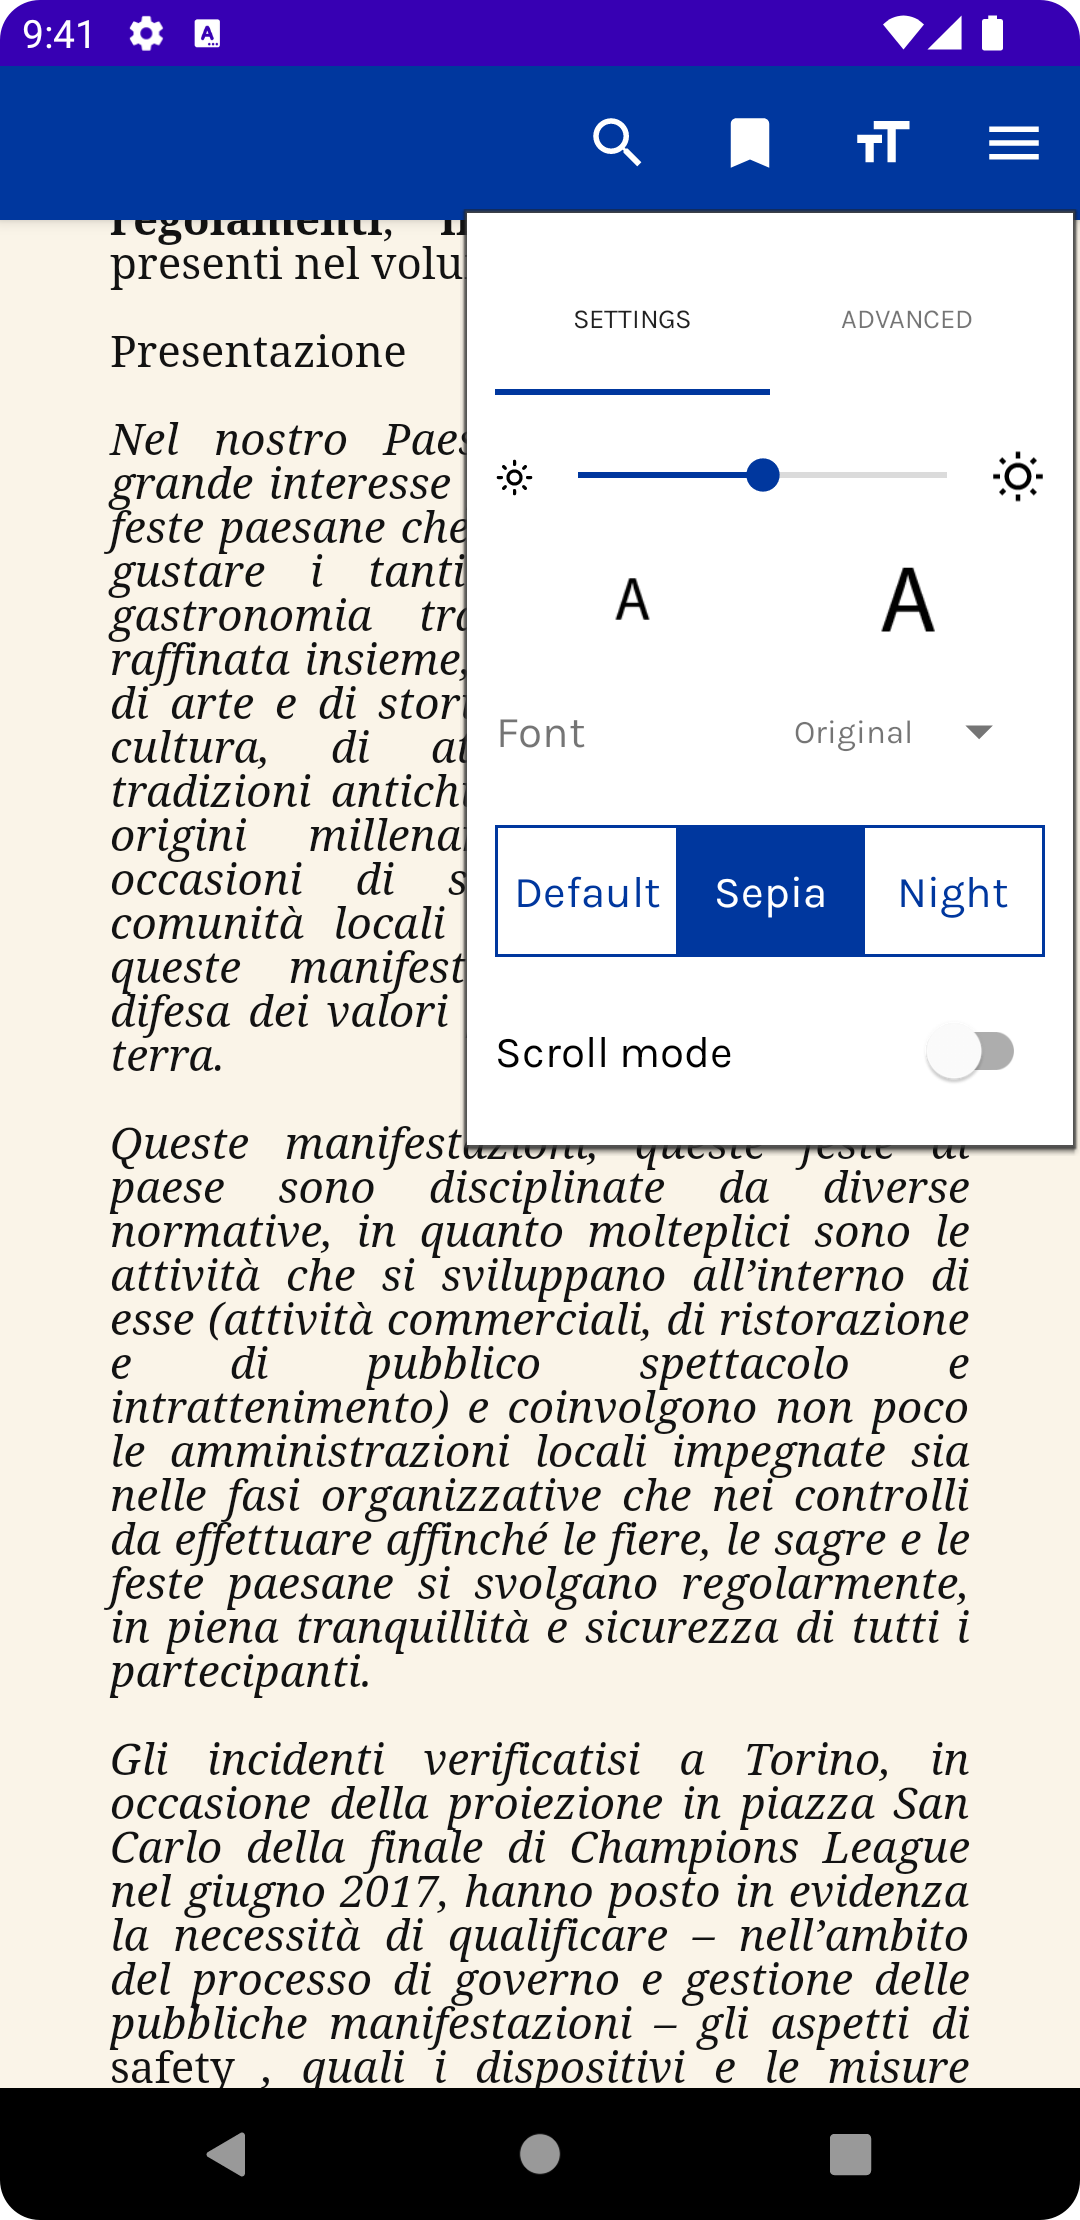
\includegraphics[width=0.21\textwidth]{img/reader_settings.png}
                \caption{Lettura documento digitale d'esempio e impostazioni del lettore}
                \label{readersettings}
            \end{figure}
            
            \begin{figure}[H]
                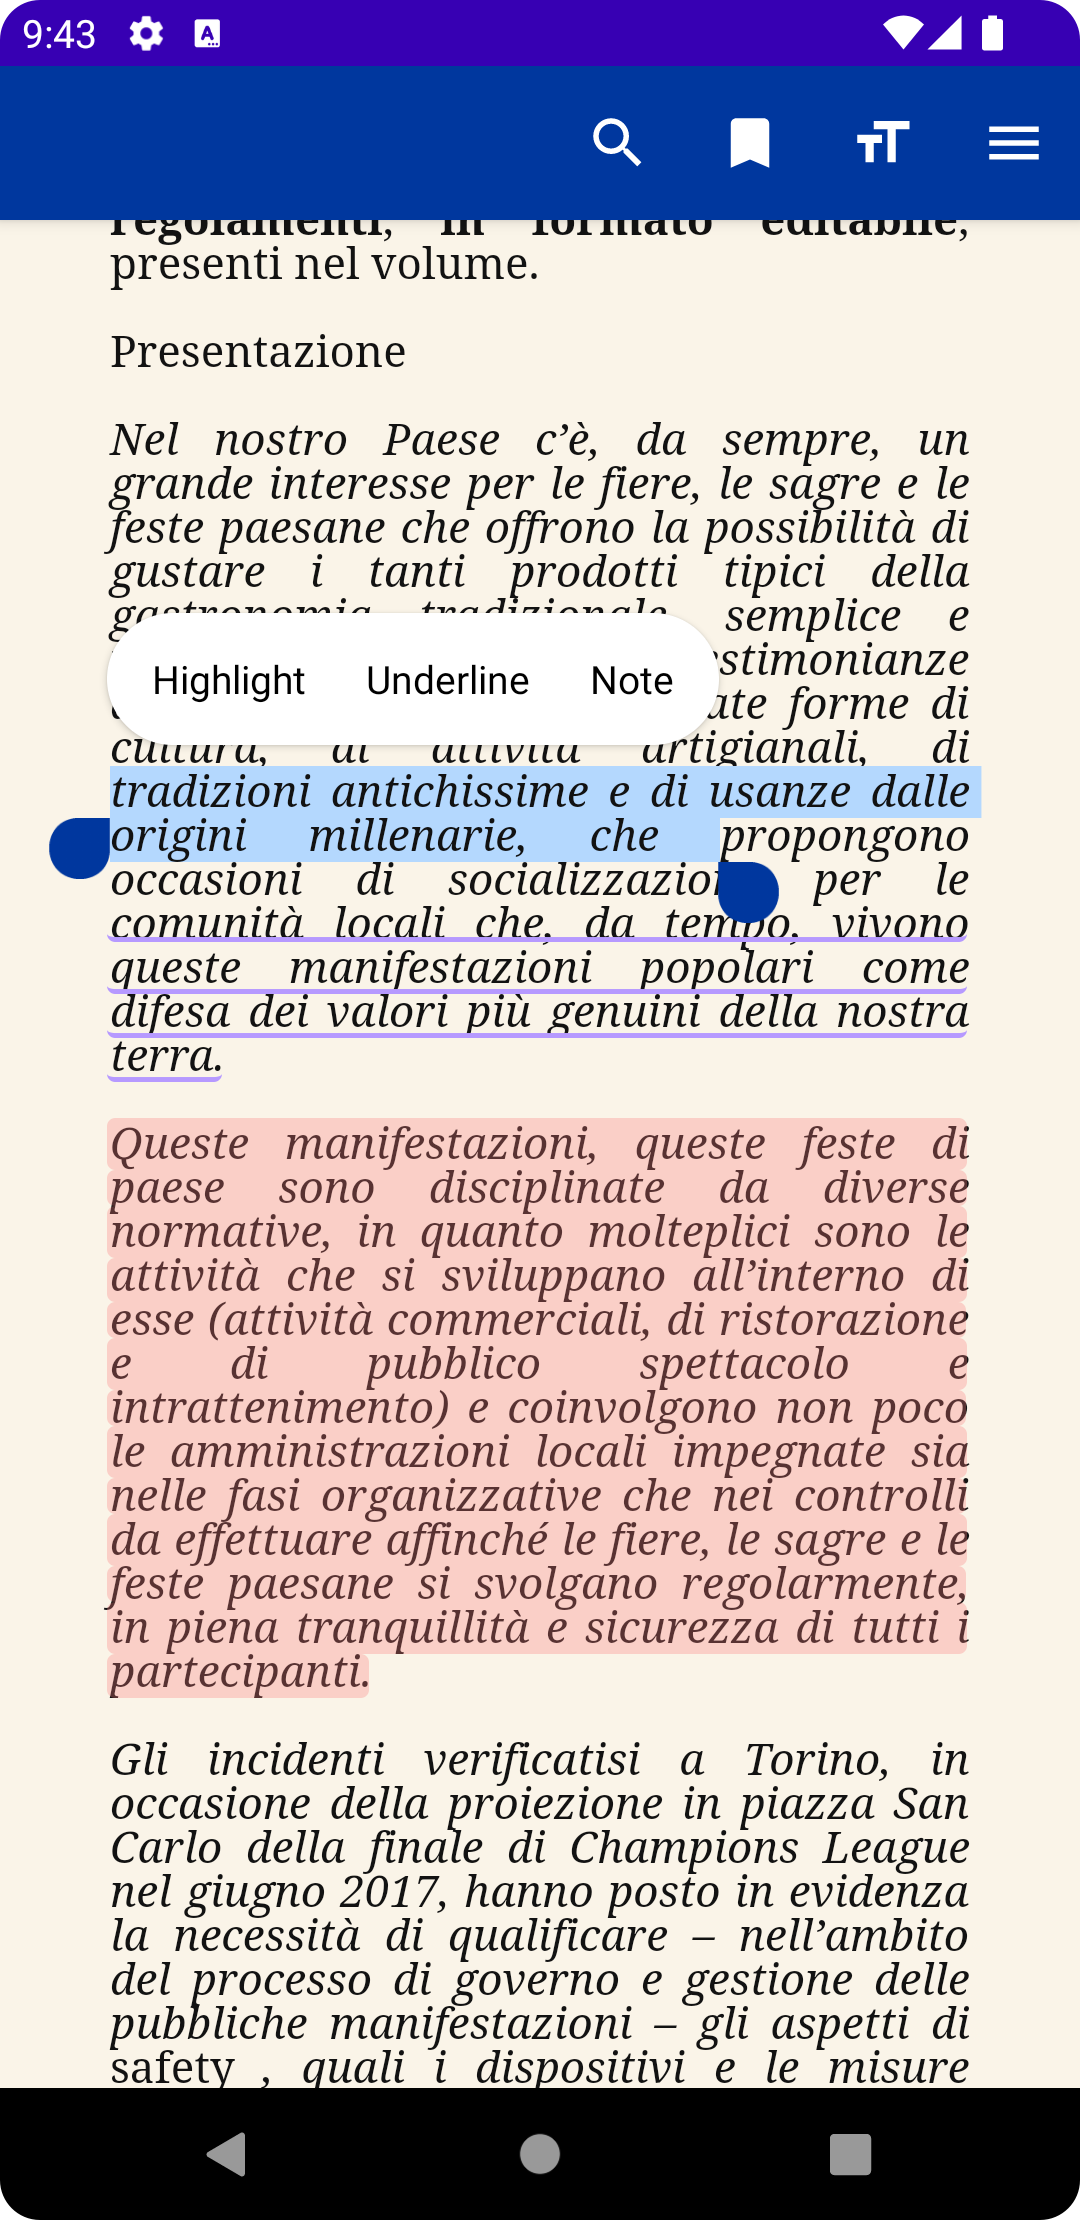
\includegraphics[width=0.21\textwidth]{img/annotations.png}
                \caption{Esempio di inserimento di annotazioni come evidenziazioni e sottolineature}
                \label{annotations}
            \end{figure}
            
            \begin{figure}[H]
                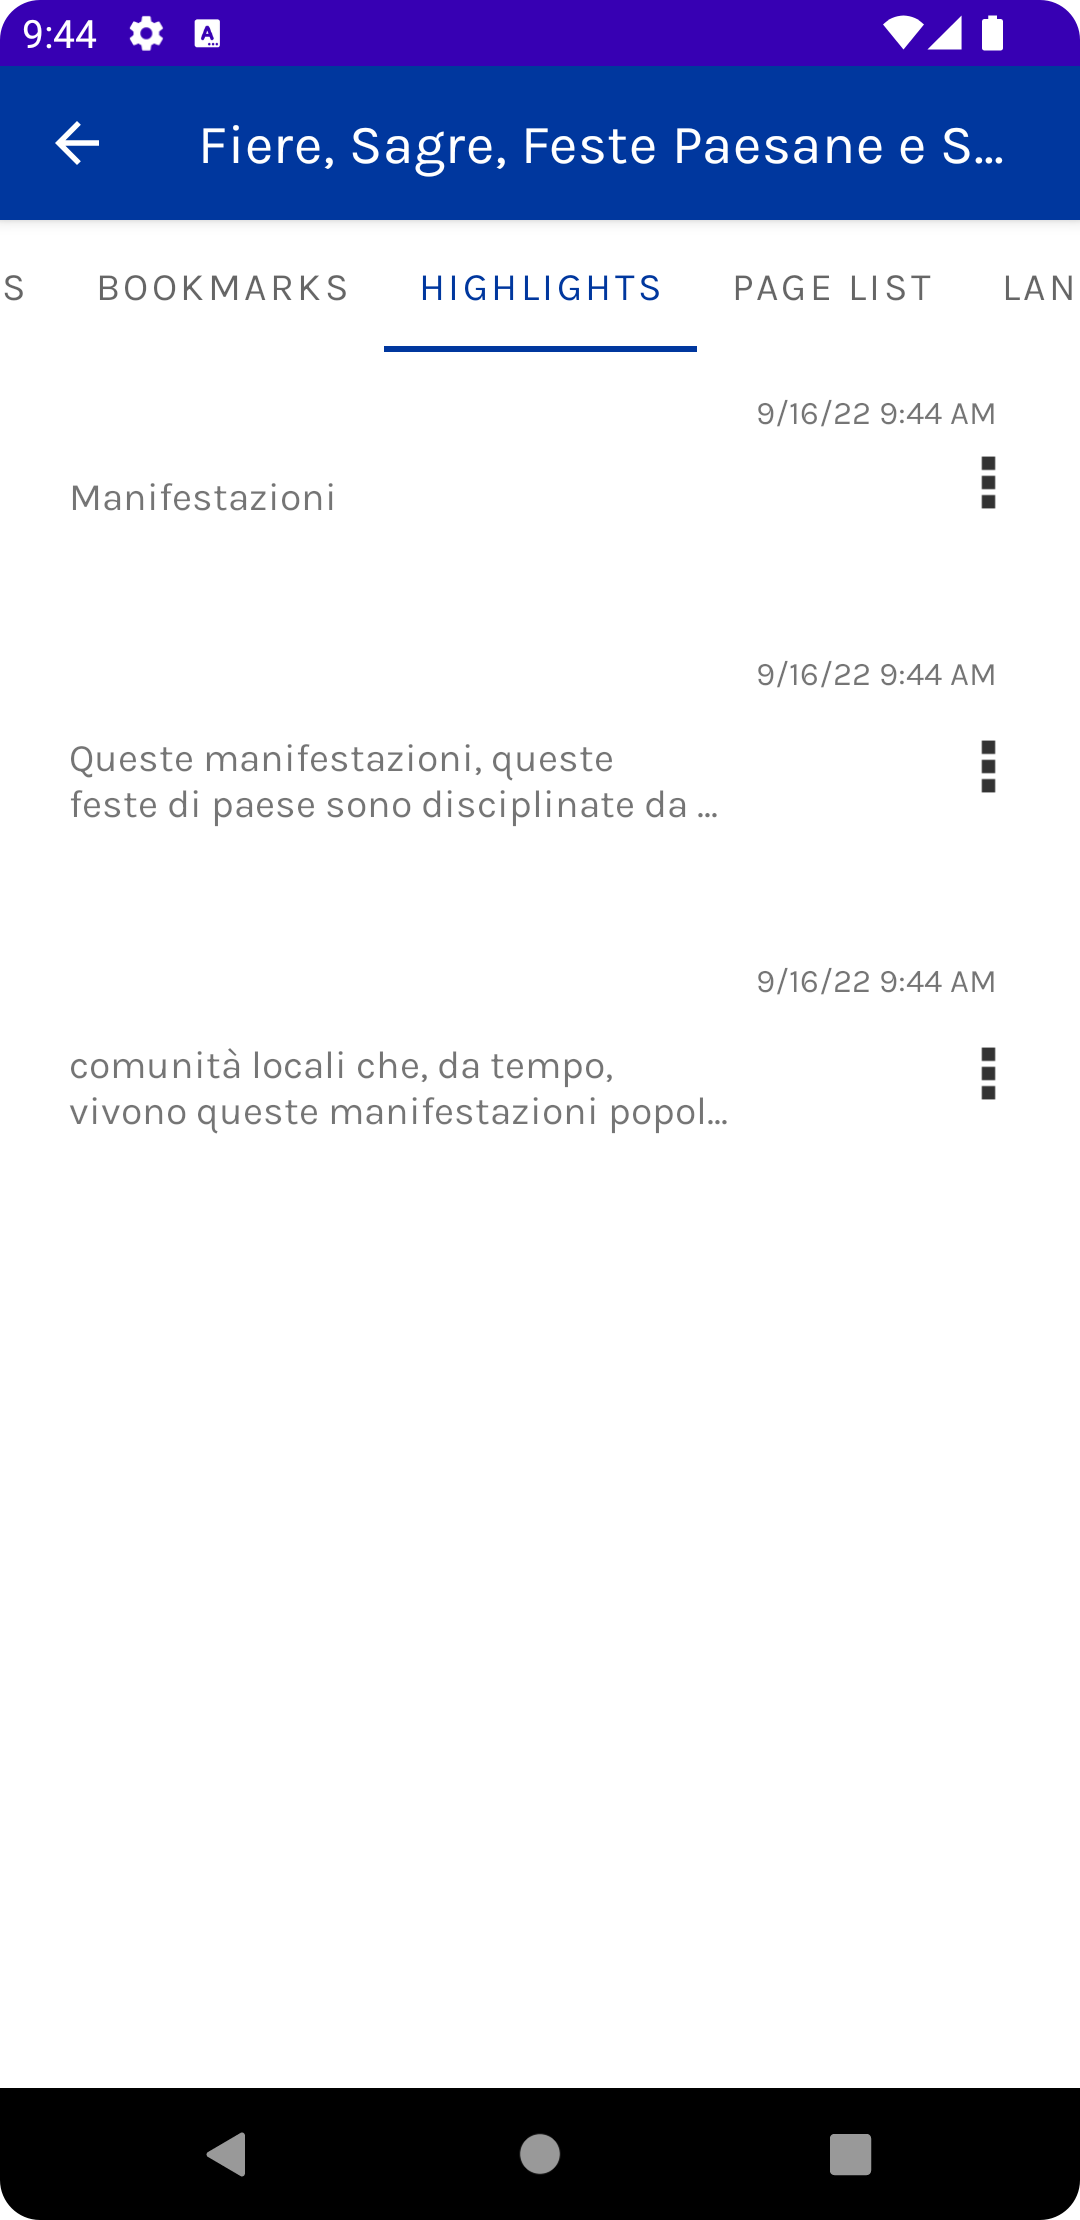
\includegraphics[width=0.21\textwidth]{img/annotation2.png}
                \caption{Annotazioni memorizzate sul dispositivo e consultabili dal menu del lettore}
                \label{annotation2}
            \end{figure}

            \begin{figure}[H]
                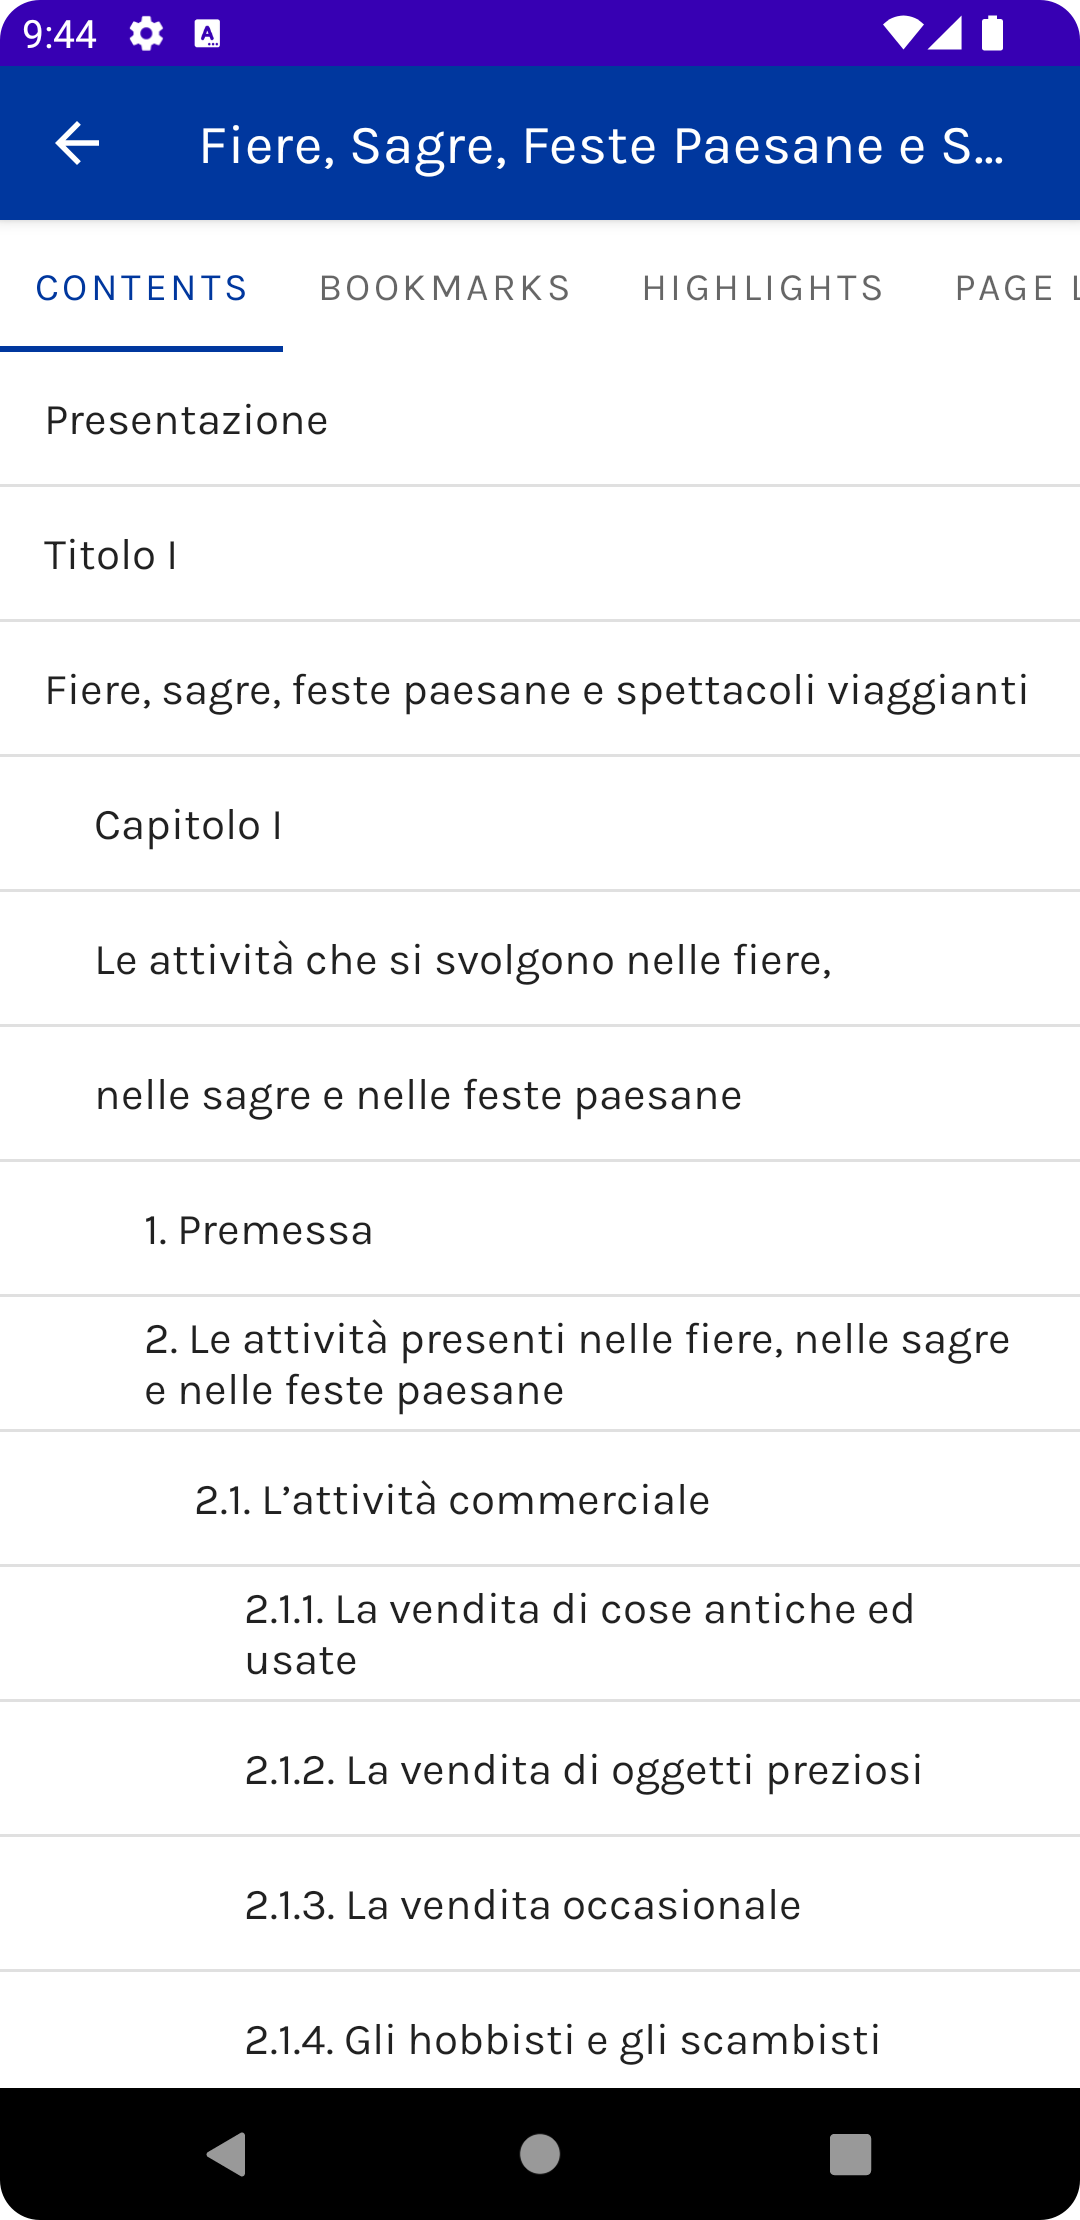
\includegraphics[width=0.21\textwidth]{img/toc.png}
                \caption{Elenco dei contenuti (TOC) del documento aperto e consultabile dal menu del lettore}
                \label{toc}
            \end{figure}
            
            \begin{figure}[H]
                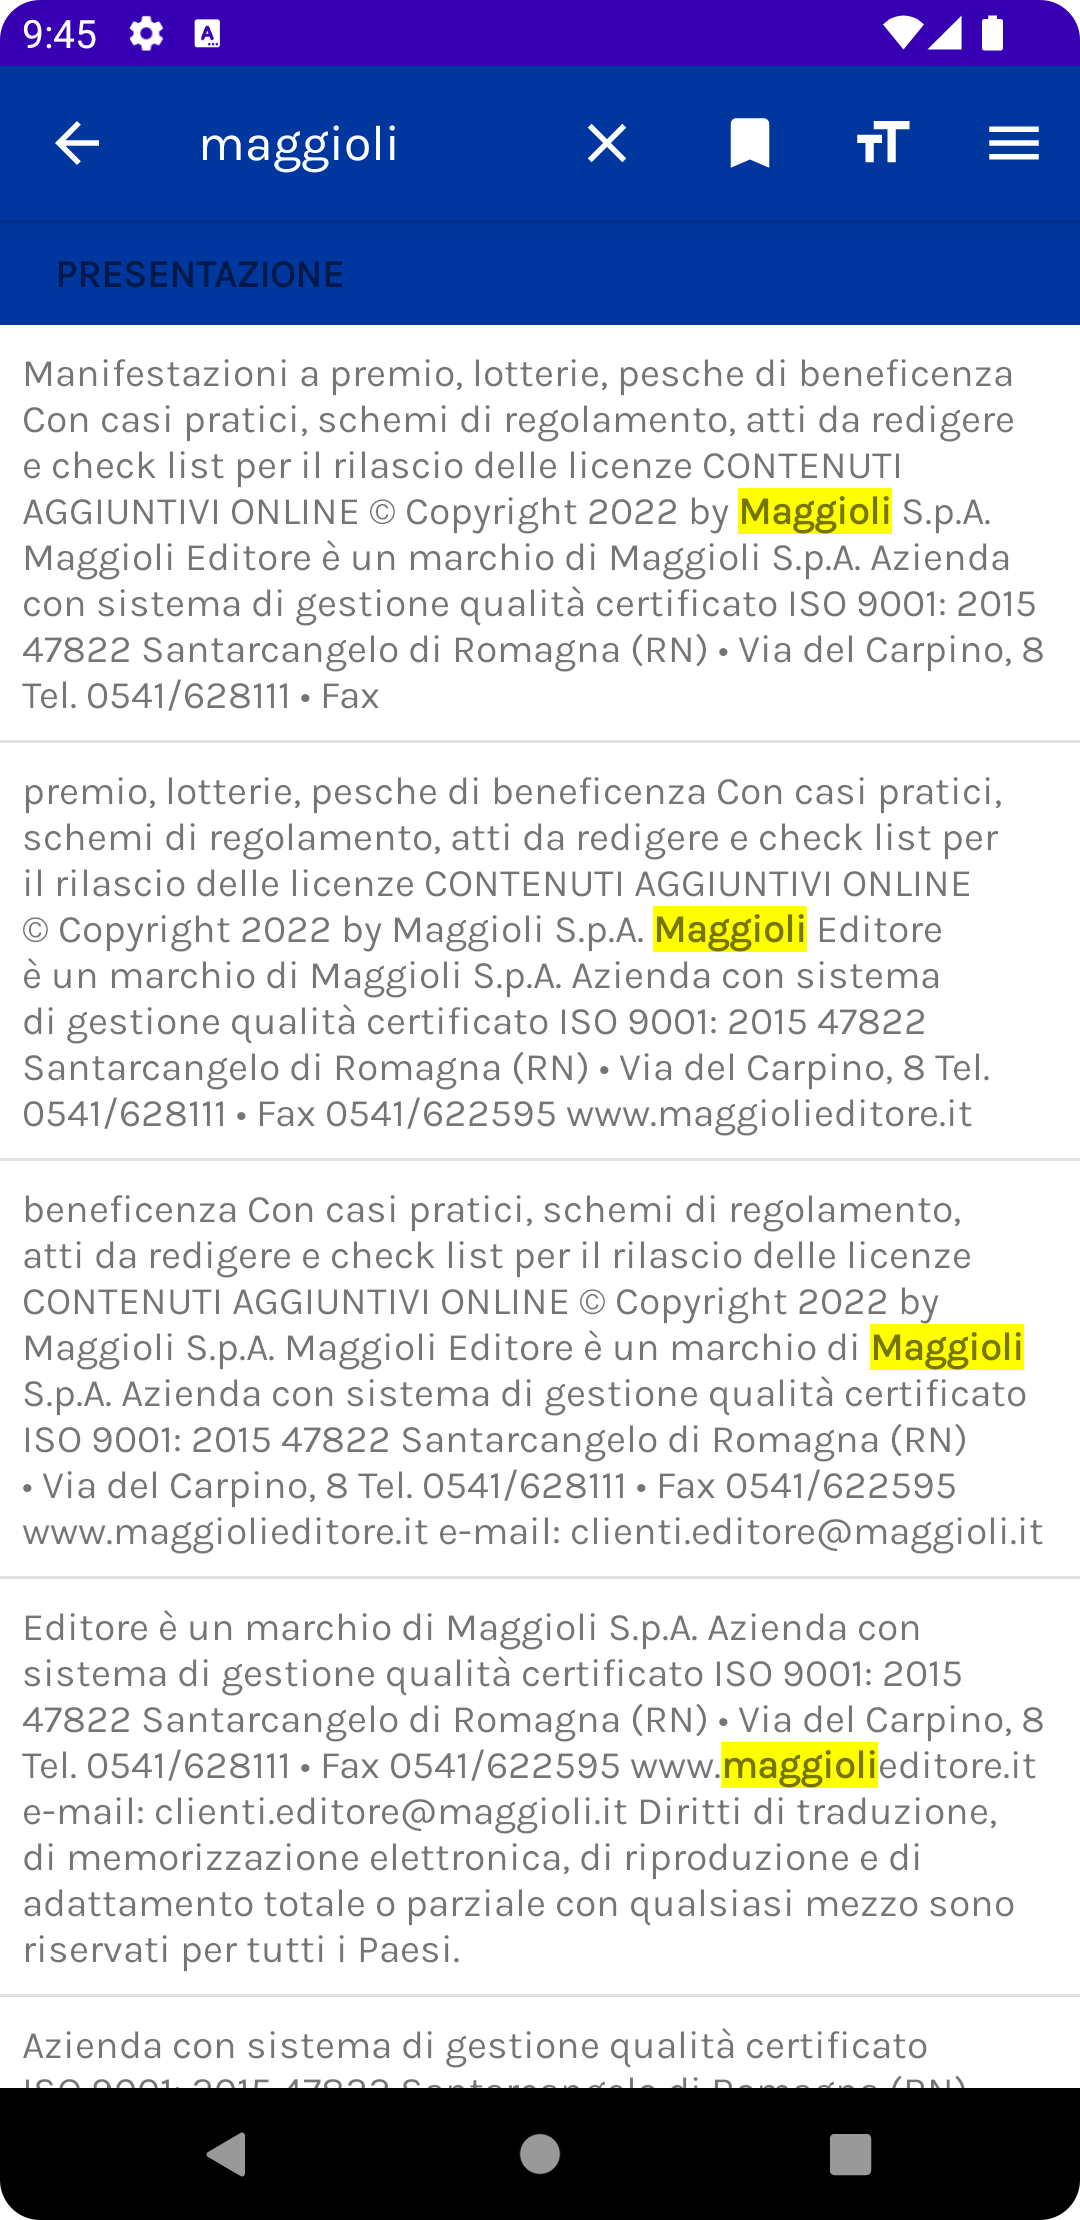
\includegraphics[width=0.21\textwidth]{img/ricerca_testo.png}
                \caption{Ricerca testuale nel contenuto del documento aperto con relativo risultato}
                \label{ricerca_testo}
            \end{figure}
            
            \begin{figure}[H]
                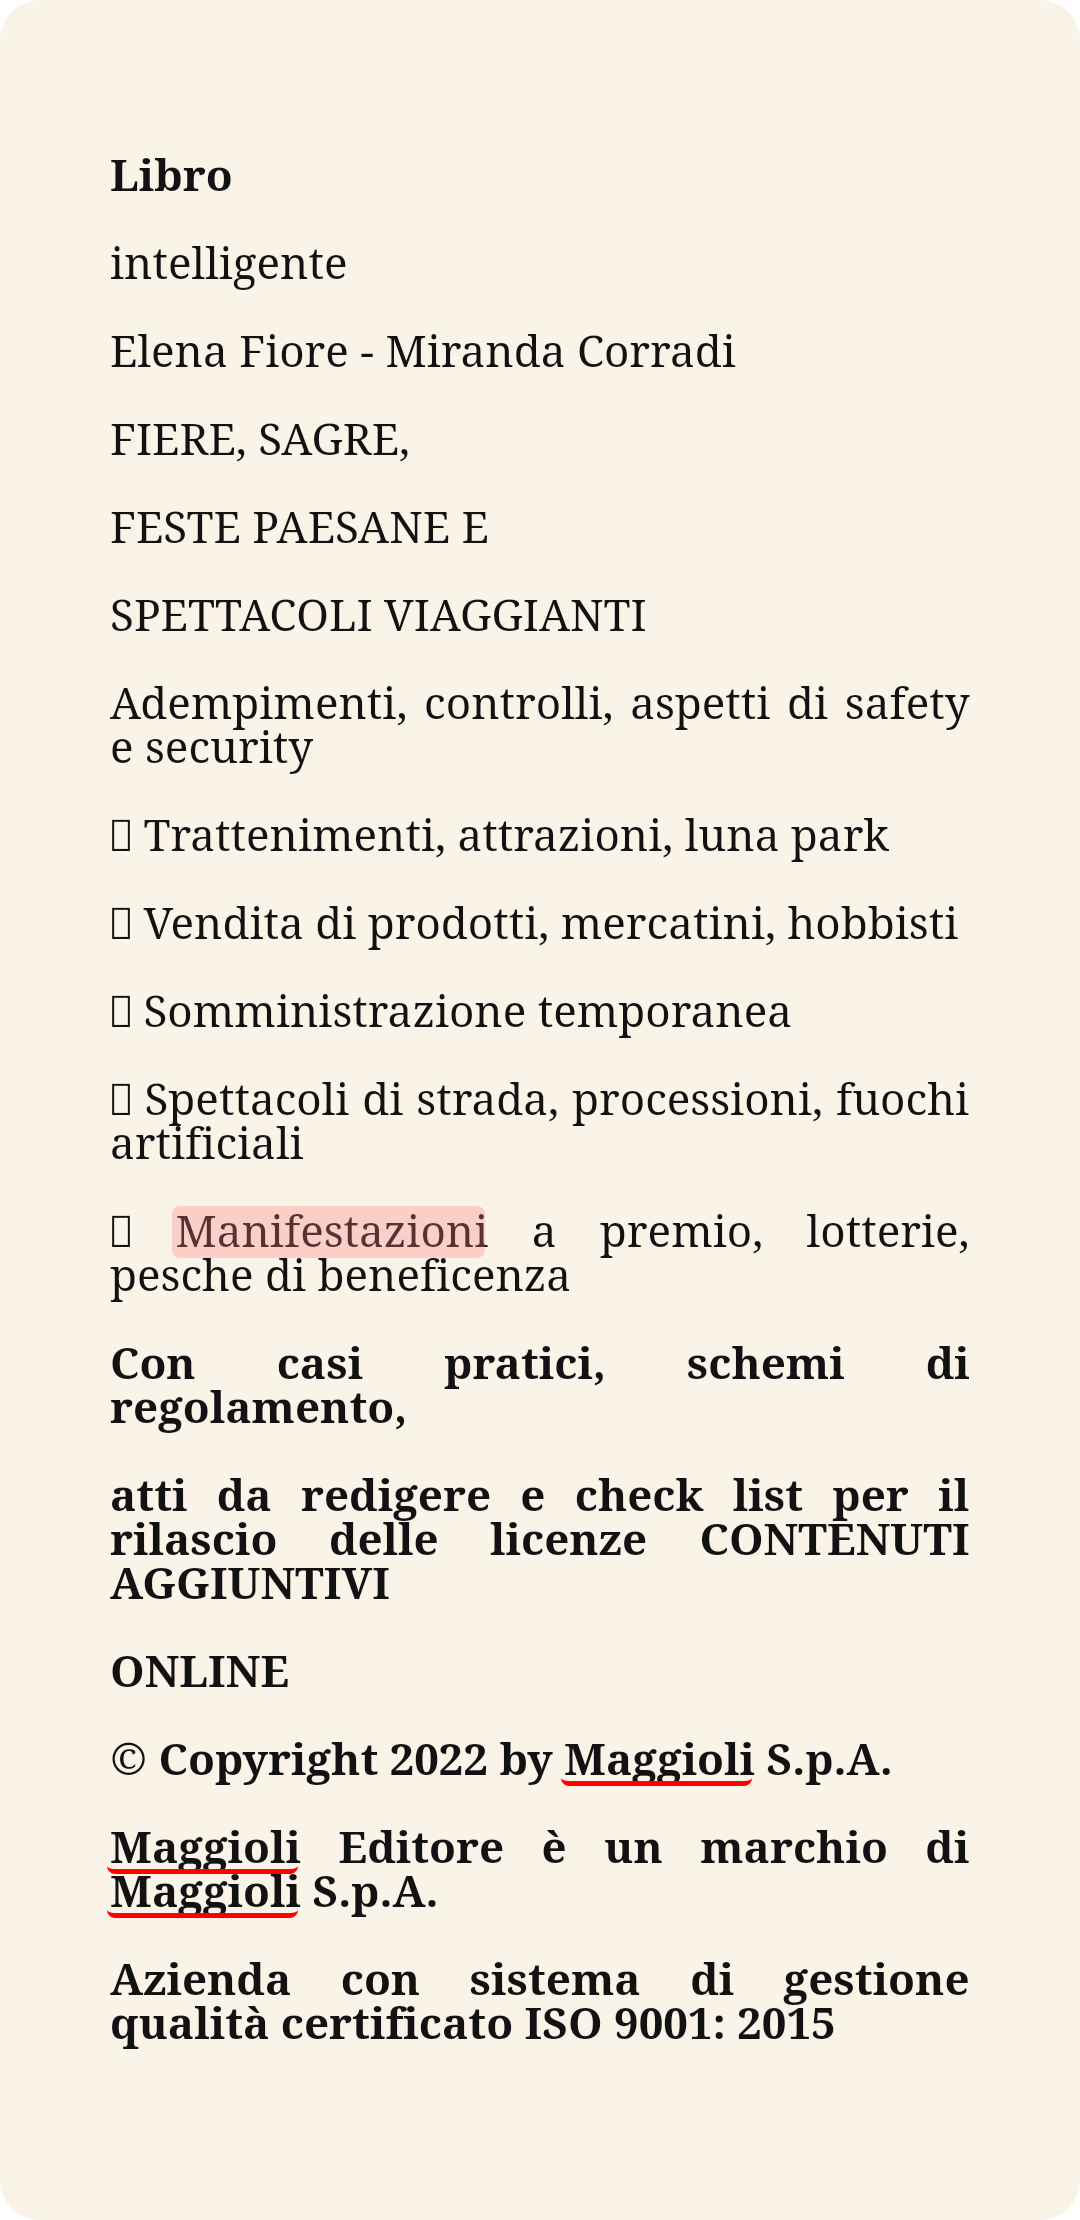
\includegraphics[width=0.21\textwidth]{img/ricerca_testo2.png}
                \caption{Evidenziazioni automatiche delle occorrenze del testo cercato}
                \label{ricerca_testo2}
            \end{figure}
\end{multicols}

\subsection{iosMaggioliEbookApp}

\chapter{Conclusioni}
\label{ch:ch6}
% !TeX root = ../main.tex

% dire i risultati ottenuti, cosa non è stato fatto e cosa si farà in futuro

Lavori futuri: 
\begin{itemize}
% lavori futuri processo di sviluppo app mobile
    \item monitoring applicazione e utente
    \item remote configuration\footnote{\url{https://firebase.google.com/docs/remote-config}} in modo da modificare aspetti della app senza dover rilasciare una nuova applicazione (esempio: migro un database, devo cambiare il jdbc url, modifico il valore invece che rilasciare una nuova app)
    \item valutare l'utilizzo di vm mac oppure immagine docker macos\footnote{\url{https://github.com/sickcodes/Docker-OSX}}
    \item valutare soluzioni complete as a service, tipo Bitrise\footnote{\url{https://www.bitrise.io/}} o xcode cloud\footnote{\url{https://developer.apple.com/documentation/xcode/xcode-cloud}}.
    \item sperimentare cicd con tecnologie cross-platform tipo ionic e con stesso caso di studio
    % lavori futuri applicazione specifica maggioliebook
    \item aggiungere supporto alla visualizzazione diretta dei pdf
    \item gestire contenuti aggiuntivi del epub oltre a highlights, bookmark ecc come ad esempio quiz, link esterni, ecc
\end{itemize}

\end{comment}

\addcontentsline{toc}{chapter}{Bibliografia}
\bibliographystyle{plain}
\bibliography{main}

\end{document}
